\documentclass[letterpaper,12pt,leqno]{article}


\usepackage{paper}


%\usepackage{natbib}
%\bibliographystyle{bibliography}
\bibliographystyle{plainnat}
%\bibliographystyle{alpha}
% Enter paper title:
\hypersetup{pdftitle={Paper Example}}
\graphicspath{{./graphs/}{./graphs/lalonde/}{./graphs/irs}{./graphs/tables}}%

% add blank page
\usepackage{afterpage}
\newcommand\blankpage{\null\thispagestyle{empty}  \addtocounter{page}{-1}\newpage}

%\usepackage[colorlinks,linkcolor=CardinalRed,citecolor=CardinalRed,urlcolor = CardinalRed]{hyperref}

% yiqing adds: no indent for footnotes
\usepackage[flushmargin]{footmisc}
\setlength{\footnotemargin}{2mm}


% guido adds


\newcommand{\indep}{\perp\!\!\!\perp}

\usepackage[colorinlistoftodos]{todonotes}
\usepackage{placeins}

\newcommand{\guido}[1]{
    \todo[inline,color=orange!50]{
    \textbf{Guido:}   #1    }}


\newcommand{\yiqing}[1]{
    \todo[inline,color=blue!50]{
    \textbf{Yiqing:}    #1    }}




% Enter permanent URL to paper
%\available{xxx}

% Enter BibTeX file with references:
\newcommand{\bib}{main.bib}

% Enter PDF file with figures here:
\newcommand{\pdf}{figures.pdf}

%

%\newcommand{\msquare}{\magenta{$\blacksquare$}\ }
%\newcommand{\bdiamond}{\blue{$\diamond$}\ }
%\newcommand{\mdiamond}{\magenta{$\diamond$}\ }

\newtheorem{result}{Result}
\newtheorem{example}{Example}
\newtheorem{comments}{Comment}

% Argmax and Argmin
\DeclareMathOperator*{\argmin}{arg\,min}
\DeclareMathOperator*{\argmax}{arg\,max}

\iffalse
\setcounter{MaxMatrixCols}{10}
\renewcommand{\mathbf}{\boldsymbol}
\setlength{\topmargin}{0.25in}
\setlength{\textheight}{8.25in}
\setlength{\evensidemargin}{-0.125in}
\setlength{\oddsidemargin}{-0.125in}
\setlength{\textwidth}{6.75in}
\renewcommand{\thepage}{}
\fi

\renewcommand{\appendix}{\footnotesize\parindent 0cm\setcounter{equation}{0}
	\renewcommand{\theequation}{A.\arabic{equation}}
	\setcounter{lemma}{0}\renewcommand{\thelemma}{A.\arabic{lemma}}}




%\numberwithin{result}{chapter}
%\numberwithin{proposition}{chapter}
%\numberwithin{theorem}{chapter}
%\numberwithin{assumption}{chapter}
%\numberwithin{lemma}{chapter}
%\numberwithin{definition}{chapter}
%\numberwithin{example}{chapter}


\newcommand{\ar}{{\rm AR}}
\newcommand{\ad}{{\rm ad}}
\newcommand{\ability}{{\rm ability}}
\newcommand{\always}{{\rm always-taker}}
\newcommand{\aand}{{\hskip1cm {\rm and}\ \ }}
\newcommand{\ave}{{\rm ave}}
\newcommand{\aven}{\frac{1}{N}\sum_{i=1}^N}
\newcommand{\alphas}{\alpha^*}
\newcommand{\atsign}{$0$}

\newcommand{\bootstrap}{\mathrm{boot}}
\newcommand{\bepsilon}{\mathbf{\varepsilon}}
\newcommand{\been}{{\bf 1}}
\newcommand{\betas}{\beta^*}
\newcommand{\betablp}{\beta_\blp}
\newcommand{\bg}{{\bf G}}
\newcommand{\bi}{{\bf I}}
\newcommand{\blp}{{\rm blp}}
\newcommand{\bp}{{\bf P}}
\newcommand{\bpx}{{{\bf P}_{\bf X}}}
\newcommand{\by}{{\bf Y}}
\newcommand{\bx}{{\bf X}}
\newcommand{\br}{{\bf R}}
\newcommand{\bw}{{\bf W}}
\newcommand{\bww}{{\bf w}}
\newcommand{\brr}{{\bf r}}
\newcommand{\ba}{{\bf A}}
\newcommand{\bz}{{\bf Z}}
\renewcommand{\bv}{{\bf V}}
\newcommand{\bs}{{\bf S}}



\newcommand{\cals}{{\cal S}}
\newcommand{\calh}{{\cal H}}
\newcommand{\calt}{{\cal T}}
\newcommand{\ccc}{{\cal C}}
\newcommand{\ccb}{{\cal S}}
\newcommand{\ccr}{{\cal R}}
\newcommand{\caln}{{\cal N}}
\newcommand{\calg}{{\cal G}}
\newcommand{\calp}{{\cal P}}
\newcommand{\ccii}{{\rm CI}}
\newcommand{\ca}{\mathbb{A}}
\newcommand{\ci}{{\rm CI}}
\newcommand{\comp}{{\rm complier}}
\newcommand{\ct}{{\rm c}}
\newcommand{\combined}{{\rm comb}}

\newcommand{\data}{\mathrm{data}}
\newcommand{\did}{\mathrm{DID}}
\newcommand{\donald}{\mathrm{Donald}}
\newcommand{\dif}{{\rm dif}}

\newcommand{\emphunderline}{\underline}
\newcommand{\earn}{{\rm earnings}}
\newcommand{\educ}{{\rm educ}}
\newcommand{\exper}{{\rm exper}}
\newcommand{\expers}{{\rm exper}^2}
\newcommand{\el}{{\rm el}}
\newcommand{\ehw}{{\rm EHW}}
\newcommand{\ehww}{{\rm ehw}}

\newcommand{\ff}{{\rm f}}
\newcommand{\fs}{{\rm fs}}
\newcommand{\frd}{{\rm frd}}
\newcommand{\finsin}{\frac{1}{N}\sum_{i=1}^N}
\newcommand{\fin}{\frac{1}{N}}

\newcommand{\gary}{\mathrm{Gary}}
\newcommand{\gls}{{\rm fgls}}
\newcommand{\gs}{g}
\newcommand{\GG}{G}


\newcommand{\hmmv}{{\hat{\mathbb{V}}}}
\newcommand{\high}{{\rm high}}
\newcommand{\hct}{{\rm HC2}}
\newcommand{\hcth}{{\rm HC3}}
\newcommand{\homo}{\mathrm{homo}}
\newcommand{\hatbetaols}{\hat\beta^{\rm ols}}
\newcommand{\hatthetagmm}{\hat\theta_{\rm gmm}}
\newcommand{\hatthetael}{\hat\theta_{\rm el}}
\newcommand{\hatthetaml}{\hat\theta_{\rm ml}}
\newcommand{\htau}{\hat{\tau}}

\newcommand{\iv}{\mathrm{IV}}


\newcommand{\josh}{\mathrm{Josh}}
\newcommand{\jack}{\mathrm{jacknife}}

\newcommand{\lambdas}{\lambda^*}
\newcommand{\lb}{{\rm lb}}
\newcommand{\liml}{{\rm liml}}
\newcommand{\learn}{{\rm log(earnings)}}
\newcommand{\lectures}{{Lectures in Econometrics,\ }}

\newcommand{\mrelec}{\mathrm{elec}}
\newcommand{\mrcap}{\mathrm{cap}}
\newcommand{\mroper}{\mathrm{oper}}
\newcommand{\mrno}{\mathrm{no}}
\newcommand{\mrgas}{\mathrm{gas}}
\newcommand{\medd}{{\rm med}}
\newcommand{\mm}{{\rm m}}
\newcommand{\med}{{\rm med}}
\newcommand{\mle}{{\rm mle}}
\newcommand{\mmr}{{\mathbb{R}}}
\newcommand{\mmw}{{\mathbb{W}}}
\newcommand{\mmz}{\mathbb{Z}}
\newcommand{\mx}{\mathbb{X}}
\newcommand{\ml}{{\rm ml}}
\newcommand{\mme}{{\mathbb{E}}}
\newcommand{\mmv}{{\mathbb{V}}}
\newcommand{\mma}{{\mathbb{A}}}
\newcommand{\mmva}{{\mathbb{AV}}}
\newcommand{\mmc}{{\mathbb{C}}}
\newcommand{\mmx}{{\mathbb{X}}}
\newcommand{\modrobust}{{\rm HC2}}
\newcommand{\mvar}{\mathbb{V}}
\newcommand{\mmav}{{\mathbb{AV}}}


\newcommand{\nfn}{N_{{\rm f}\ct}}
\newcommand{\nmn}{N_{{\rm m}\ct}}
\newcommand{\nfe}{N_{{\rm f}\tc}}
\newcommand{\nme}{N_{{\rm m}\tc}}
\newcommand{\never}{{\rm never-taker}}
\newcommand{\nc}{N_{\ct}}
\newcommand{\nt}{N_{\tc}}
\newcommand{\nf}{N_{\ff}}
\newcommand{\nm}{N_{\mm}}
\newcommand{\neyman}{\mathrm{neyman}}

\newcommand{\opsn}{o_p\left(N^{-1/2}\right)}
\newcommand{\Opsn}{O_p\left(N^{-1/2}\right)}
\newcommand{\opn}{o_p\left(N^{-1}\right)}
\newcommand{\Opn}{O_p\left(N^{-1}\right)}
\newcommand{\obs}{{\rm obs}}
\newcommand{\oy}{\overline{Y}}
\newcommand{\orr}{\overline{R}}
\newcommand{\ols}{{\rm ols}}


\newcommand{\pop}{{\rm pop}}
\newcommand{\pate}{{\rm pate}}
\newcommand{\pos}{{\rm pos}}
\newcommand{\popt}{{\rm patt}}
\newcommand{\pr}{{\rm pr}}

\newcommand{\rank}{{\rm rank}}
\newcommand{\reg}{{\rm reg}}
\newcommand{\robust}{{\rm robust}}
\newcommand{\ress}{Y_i-X_i hatbetaols}
\newcommand{\rmelec}{{\rm elec}}
\newcommand{\relec}{{\rm elec}}
\newcommand{\rmoper}{{\rm oper}}
\newcommand{\rmcap}{\mathrm{cap}}
\newcommand{\rmgas}{\mathrm{gas}}
\newcommand{\rmno}{\mathrm{no}}
\newcommand{\rmif}{{\rm if}}

\newcommand{\qob}{{\rm qob}}

\newcommand{\subs}{\mathrm{subsampling}}
\newcommand{\sate}{{\rm sate}}
\newcommand{\sample}{{\rm sample}}
\newcommand{\samplet}{{\rm satt}}
\newcommand{\spp}{{\rm sp}}
\newcommand{\srd}{{\rm srd}}
\newcommand{\se}{{\rm s.e.}}
\newcommand{\strata}{{\rm strat}}
\newcommand{\susan}{\mathrm{Susan}}
\newcommand{\snn}{\sum_{i=1}^N}
\newcommand{\str}{^{*}}

\newcommand{\tc}{{\rm t}}
\newcommand{\tsls}{{\rm tsls}}
\newcommand{\tmle}{\hat\theta^{\rm mle}}
\newcommand{\thetaml}{\theta^{\rm mle}}
\newcommand{\ty}{\tilde Y}
\newcommand{\tick}{\checkmark}
\newcommand{\thetas}{\theta^*}
\newcommand{\taup}{\tau_\spp}
\newcommand{\tautp}{\tau_{\spp,\tc}}


\newcommand{\ow}{\overline{W}}
\newcommand{\oz}{\overline{Z}}
\newcommand{\ox}{{\overline{X}}}

\newcommand{\ub}{{\rm ub}}

\newcommand{\veen}{{\rm homo}}
\newcommand{\vtweea}{{\rm    homo,unbiased}} 
\newcommand{\vtwee}{{\rm homo,unbiased,t-dist}}
\newcommand{\vdrie}{{\rm robust}} 
\newcommand{\vet}{{\rm veteran}}

\newcommand{\wb}{{\bf W}}
\newcommand{\win}{W_{i}}
\newcommand{\welch}{\mathrm{welch}}

\newcommand{\xbj}{{\bf X}_{(j)}}
\newcommand{\xb}{{\bf X}}
\newcommand{\xbi}{{\bf X}_{(i)}}
\newcommand{\xxb}{{\bf x}}

\newcommand{\yoin}{Y_{i}}
\newcommand{\yin}{Y_i(0)}
\newcommand{\yie}{Y_i(1)}
\newcommand{\yinn}{Y_{i}(0)}
\newcommand{\yien}{Y_{i}(1)}
\newcommand{\ybn}{{\bf Y}(0)}
\newcommand{\ybe}{{\bf Y}(1)}
\newcommand{\yb}{{\bf Y}}
\newcommand{\ybo}{{\bf Y}^{\rm obs}}
\newcommand{\ybm}{{\bf Y}^{\rm mis}}
\newcommand{\yybn}{{\bf y}(0)}
\newcommand{\yybe}{{\bf y}(1)}
\newcommand{\ybni}{{\bf Y}_{(i)}(0)}
\newcommand{\ybei}{{\bf Y}_{(i)}(1)}
\newcommand{\ybnj}{{\bf Y}_{(j)}(0)}
\newcommand{\ybej}{{\bf Y}_{(j)}(1)}
\newcommand{\yoi}{Y^{\rm obs}_i}

\newcommand{\zin}{Z_{i}}
\newcommand{\indep}{\perp\!\!\!\perp}



% Fill out paper:
\begin{document}
\title{LaLonde (1986) after Nearly Four Decades:\\Lessons Learned}
\author{Guido Imbens \and Yiqing Xu
\thanks{Guido Imbens, Stanford University. Email: \url{imbens@stanford.edu}. Yiqing Xu, Stanford University. Email: \url{yiqingxu@stanford.edu}.
%Author 2: University 2. 
We thank Susan Athey, Alexis Diamond, Dean Eckles, and Scott Cunningham for comments, 
%many colleagues for helpful comments and discussions. 
the Office of Naval Research for support under grant numbers N00014-17-1-2131 and N00014-19-1-2468 and Amazon for a gift. Data and code required to replicate the analyses in this paper, as well as an online tutorial, can be found at \url{https://github.com/xuyiqing/lalonde}. We thank Zihan Xie and Jinwen Wu for their excellent research assistance, which makes the tutorial possible.}}
\date{\today}                       
\begin{titlepage}\maketitle

\vspace{-2em}\begin{abstract}\noindent
In 1986, Robert LaLonde published an article that compared nonexperimental estimates to experimental benchmarks \citep{LaLonde}. He concluded that the nonexperimental methods at the time could not systematically replicate experimental benchmarks, casting doubt on the credibility of these methods. Following LaLonde's critical assessment, there have been significant methodological advances and practical changes, including ($i$) an emphasis on estimators based on unconfoundedness, ($ii$) a focus on the importance of overlap in covariate distributions, ($iii$) the introduction of propensity score-based methods leading to doubly robust estimators, ($iv$) a greater emphasis on validation exercises to bolster research credibility, and ($v$) methods for estimating and exploiting treatment effect heterogeneity.  To demonstrate the practical lessons from these advances, we reexamine the LaLonde data and the Imbens-Rubin-Sacerdote lottery data. We show that modern methods, when applied in contexts with sufficient covariate overlap, yield robust estimates for the adjusted differences between the treatment and control groups. However, this does not mean that these estimates are valid. To assess their credibility, validation exercises (such as placebo tests) are essential, whereas goodness of fit tests alone are inadequate. Our findings highlight the importance of closely examining the assignment process, carefully inspecting overlap, and conducting validation exercises when analyzing causal effects with nonexperimental data.
\end{abstract}



\end{titlepage}


%\listoftodos


\clearpage


\section{Introduction}\label{s:introduction}

In 1986, Robert LaLonde published a paper \citep{LaLonde} based on part of his PhD thesis, which has had a profound impact on both methodological and empirical literature on estimating causal effects.\footnote{As of May 2024, it has been cited 2900 times, but this number does not do justice to its influence on the causal inference literature and the credibility revolution.}
In his paper, he assessed whether the then state-of-the-art nonexperimental evaluation methods could match experimental benchmarks. LaLonde's conclusion was quite negative regarding the credibility of the nonexperimental methods he examined. He wrote:
\begin{quote}
``This comparison shows that many of the econometric procedures do not replicate the experimentally determined results, and it suggests that researchers should be aware of the potential for specification errors in other nonexperimental evaluations.'' \cite[Abstract, p. 604]{LaLonde},
\end{quote}
and eventually concluding that
\begin{quote}
``policymakers should be aware that the available nonexperimental evaluations of employment and training programs may contain large and unknown biases resulting from specification errors.'' \cite[Conclusion, p. 617]{LaLonde},
\end{quote}
A year earlier LaLonde's thesis advisors Orley Ashenfelter and David Card had raised similar concerns:
\begin{quote}
``we conclude that randomized clinical trials are
necessary to reliably determine program effects.''   \cite[Abstract, p. 648]{ashenfelter1985using}
\end{quote}
Quickly after the publication of LaLonde's paper, several other studies echoed LaLonde's concern about the credibility of nonexperimental methods in the context of the evaluation of labor market programs \citep{fraker1987adequacy, heckman1987we}, leading to further skepticism about their value. More generally, \citet{leamer1983let} had earlier raised concerns about the credibility of applied econometric methods in nonexperimental evaluations, and asked ``Is Randomization Essential?'' \cite[p. 31]{leamer1983let}. 

One important development that greatly increased the influence of the original LaLonde study was the accessibility of the data in the early 2000s, thanks to the work by Rajeev Dehejia and Sadek Wahba
\citep{dehejiawahba, dehejia2002propensity}.\footnote{As part of a research project starting in a graduate class taught by Imbens and Rubin at Harvard in 1996, Dehejia and Wahba obtained the original data from LaLonde, stored on tapes. They successfully located an old tape reader capable of retrieving the data. The data are now publicly available on Dehejia's website (\url{https://users.nber.org/~rdehejia/data/.nswdata2.html}) and have been extensively used in the causal inference literature on causal inference.} More recently, \citet{calonico2017women} reconstructed the female samples used in LaLonde study. Throughout the remainder of the paper, we refer to the data compiled by Dehejia and Wahba as the LaLonde-Dehejia-Wahba (LDW) data and the reconstructed female samples as the Lalonde-Cal{\'o}nico-Smith (LCS) data.


In this paper, we summarize our perspective on the lessons from the methodological literature that followed LaLonde's seminal paper. We argue that while some of LaLonde's original conclusions have stood the test of time, in our view substantial progress has been made in the methodological literature both in terms of improved estimators and in the form of suggested additional analyses. At this point, almost four decades after LaLonde's paper, the answer to his original question---whether nonexperimental methods can successfully replicate experimental benchmarks---is more nuanced than his conclusions: sometimes we can, and we now have better methods both for achieving this when we can, and for telling whether we can. We stress that these views are our own, based on our reading of, and contributions to, this literature. Many issues in this literature remain subjects of ongoing debate, and  other researchers hold different opinions on these developments.


What specifically has the methodological literature since \citet{LaLonde} taught us? What particular analyses would we recommend a researcher analyzing data of this type do in the light of the subsequent theoretical research? In this discussion, we focus on five issues related to the particular setting studied in \citet{LaLonde}, the evaluation of an intervention at the individual level, based on detailed background information on those individuals. There is a literature on causal inference more broadly which has grown substantially over the nearly four decades as well, as documented in \citet{currie2020technology}. We do not cover this broader literature here. There are more comprehensive surveys of the general causal literature,  \citep[e.g.,][]{abadie2018econometric, imbens2009recent}, as well as numerous textbooks \citep{angrist2008mostly, imbens2015causal, cunningham2018causal, huntington2021effect, huber2023causal}. Here, we limit the discussion to five lessons learned from the subsequent literature for settings similar to those in \cite{LaLonde}.

First, for the type of data used in LaLonde's paper, the literature has predominantly focused on methods based on the unconfoundedness (or, using other terms, exogeneity, ignorability, conditional independence, or selection-on-observables) assumption. Although \citet{LaLonde}, as well as \citet{heckman1989choosing} and others, explored alternative identification strategies in their analyses, including difference-in-differences and selection models, these methods are rarely applied to the LaLonde data in the subsequent literature. No compelling case has been made that other identification strategies are credible in that context. 
The lack of alternatives, of course, does not make the unconfoundedness assumption itself credible. The positive case for an analysis based on unconfoundedness is as follows: with the LaLonde data, or similar datasets, we argue that comparing treated and control untis identical or similar in terms of the full set of available pretreatment variables makes a causal interpretation more plausible than any other comparison between treated and control units. Any alternative strategy that would lead to point-identification would involve comparing treated and control units with different values for the pretreatment variables, which, in our view, makes a causal interpretation less credible. For that reason, we focus in this discussion on methods relying on unconfoundedness assumptions. For recent reviews of panel methods, see \citet{xu2023causal} and \citet{arkhangelsky2023causal}. 

Second, and this is perhaps the most important insight, the literature has recognized the crucial role of assessing overlap in covariate distributions and dealing directly with the lack thereof.  The various comparison groups \citet{LaLonde} used to evaluate nonexperimental methods all differ substantially from the experimental sample in terms of the distributions of the covariates. This creates challenges for conventional statistical adjustment methods such as regression and matching. LaLonde attempted to address these by simply discarding individuals in the comparison groups who do not meet certain specific eligibility criteria based on age, employment status and earnings. The subsequent literature has emphasized that, in practice, lack of overlap is a key issue in such analyses. Effective and systematic, data-driven, ways of diagnosing, and addressing this lack of overlap have been developed subsequently.

Third, and somewhat related to the overlap issue, the role of the propensity score in estimation has been stressed. There are two components to this role. First, the propensity score plays an important role in uncovering and addressing the lack of overlap in covariate distributions. Second, it is important in the estimation of treatment effects, either directly through inverse propensity score weighting (IPW) or, more importantly in the current state-of-the-art approaches, as part of doubly robust methods that incorporate both models for the conditional outcome distributions and the models for the propensity score. Propensity scores played no role in LaLonde's analyses. In fact, the term ``propensity score'' does not appear. The paper that introduced the propensity score, \citet{rosenbaum1983central}, and which by now has over 37,000 Google Scholar cites, had only recently been published at that time and had not yet influenced the econometrics literature.\footnote{The first mention of the propensity score in the econometrics literature appears to be \citet{card1988measuring}. Interestingly, they cite \citet{rosenbaum1984reducing}
rather than the original propensity score paper \citet{rosenbaum1983central}.} Subsequently, recognizing the importance of modeling both the assignment mechanism and the conditional outcome distribution has spurred the development of various doubly robust methods. First introduced by \citet{scharfstein1999comments}, these methods are now generally viewed as the most attractive methods based on unconfoundedness in practice. The incorporation of machine learning techniques into causal inference has further enabled this by reducing the need for {\it ad hoc}  specification searches. 

Fourth, scholars have come to realize the importance of establishing the credibility of estimates through validation exercises, particularly placebo analyses. \citet{LaLonde} did some placebo analyses looking at the estimated effect for lagged earnings, but primarily focused on the comparisons between nonexperimental and experimental estimates of average treatment effects. The recent empirical literature has placed significant emphasis on supporting main estimates with supplementary analyses, which often take the form of placebo analyses that present estimates of causal effects known to be zero.

Fifth, effective methods have emerged for other estimands, such as conditional average treatment effects for the treated (CATT)---conditional on (possibly high-dimensional) covariates---and quantile treatment effects. In many cases, decision-makers seek to understand not just the average effects for the entire population but also the extent and nature of effect heterogeneity, or even to estimate personalized assignment rules. Do some subpopulations benefit more from the treatment than others? Do some experience negative effects? The availability of large datasets has led to the development of effective ways of estimating heterogeneous treatment effects  \citep[{\it e.g.},][]{wager2018estimation}.

To demonstrate the insights from these five lessons, we reexamine the LaLonde data, including the LDW data, the male samples from the original LaLonde study, and the LCS female samples, using modern methods. We show that once we ensure sufficient overlap, multiple methods based on unconfoundedness yield quite similar estimates for the statistical estimand, that is, the average adjusted difference between treatment and control groups. However, these estimates often do {\it not} match experimental benchmarks for the average treatment effect on the treated (ATT). Similarly, CATT estimates and quantile treatment effect estimates do not consistently align with experimental results. Moreover, standard validation exercises based on placebo estimates do {\it not} support the unconfoundedness assumption using the LDW or LCS data. Despite these challenges, there is room for optimism. Analyzing the data from \citet*{imbensrubinsacerdote} (hereafter, the IRS data), which benefits from a clearer assignment mechanism (lottery) and more detailed pretreatment information, we find that the placebo analyses support the unconfoundedness assumption.

The rest of this paper is organized as follows. In Section \ref{findings}, we discuss LaLonde's original findings. In Section \ref{s:graphs} we discuss the methodological advances since \citet{LaLonde}. Next, in Section \ref{reanalyses}, we revisit the LaLonde data and reanalyze the IRS data. Finally, Section~\ref{conclusion} concludes with recommendations to applied researchers.

\section{LaLonde's Findings}\label{findings}

In this section, we first describe the data Lalonde used and explain the main econometric specifications of the models in \citet{LaLonde}. We then examine the regression estimates in his paper, followed by a discussion of the selection model estimates. After summarizing Lalonde's findings, we proceed to describe the Lalonde-Dehejia-Wahba data and explore some of the immediate responses to LaLonde's findings. 

\subsection{LaLonde's Data}

\citet{LaLonde} analyzed the training effects of the National Supported Work Demonstration (NSW) program for female and male participants separately. The female participants were drawn from the Aid to Families with Dependent Children (AFDC) program. The male participants came from three other target groups, all with relatively poor labor market prospects: ex-drug addicts, ex-criminal offenders, and high-school dropouts. For both female and male participants, LaLonde used two main data sources to construct comparison groups: CPS-SSA-1, drawn from Westat's Matched Current Population Survey--Social Security Administration File, includes all females or males under 55 meeting Westat's criteria; PSID-1, from the Panel Study of Income Dynamics, includes all female or male household heads under 55 from 1975 to 1978 for males and 1979 for females who did not identify as retired in 1975. the age cutoff was chosen to make the comparison group more comparable to the experimental sample. LaLonde further refined these datasets based on criteria like employment status, time of survey, and poverty status, creating four additional comparison groups: CPS-SSA-2, CPS-SSA-3, PSID-2, and PSID-3. Our subsequent reanalysis will primarily focus on the male samples because they are commonly used in methodological literature and because the LDW data include two pretreatment outcomes. Results based on the female samples are provided in the Supplementary Materials (SM). 

\begin{table}[!ht]
\caption{Descriptive Statistics: LaLonde and LDW Male Samples}\label{tb:samples}
\begin{minipage}[c]{0.9\textwidth}
\vspace{-0.5em}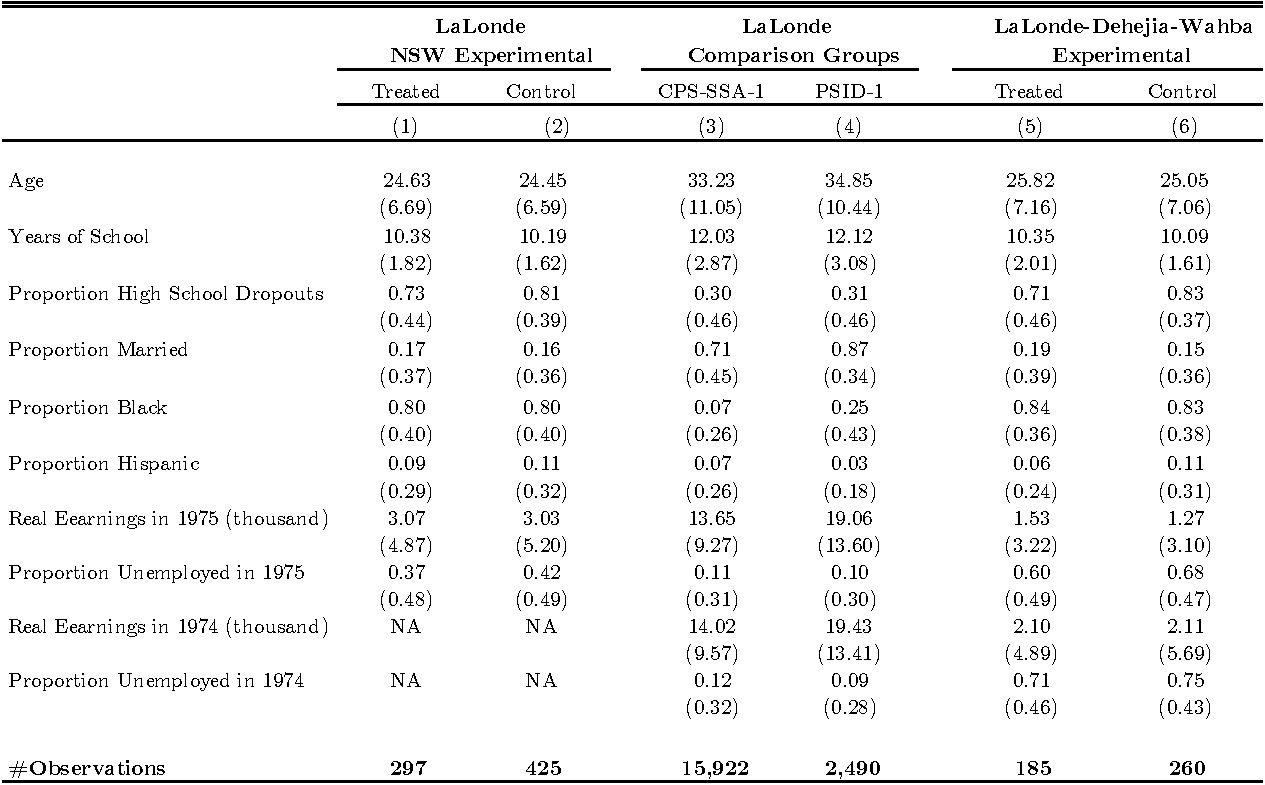
\includegraphics[width=\linewidth]{stats.pdf}
{\footnotesize\textbf{\textit{Note:}} Standard deviations are in the parentheses. Tables 3, 5, and 6 in \citet{LaLonde} use data described in columns 1--4. \cite{dehejiawahba} primarily use data described in columns 3--6.}
\end{minipage}%
\end{table}

Table~\ref{tb:samples} columns 1--4 provide summary statistics for the male samples in the experimental data and comparison groups used in \citet{LaLonde}. LaLonde showed that respondents in the comparison groups were, on average, older, more educated, substantially less likely to be high school dropouts, more likely to be married, and less likely to be Black or Hispanic, than participants of the NSW experiment; they also had substantially higher earnings in years before the program took place. The large difference in average earnings between the comparison groups and the experimental sample motivated LaLonde to construct the other comparison groups, using earnings-based criteria.
Note that the male CPS-SSA-1 sample, with 15,922 observations, is significantly larger than the male PSID-1 sample, which has 2,490 observations. 

The experimental treated units in the LDW data are a subset of the treated units in the original LaLonde data, specifically chosen to include information on 1974 earnings. Using this subset turns out to be important as it allows analysts to adjust longer earnings histories and conduct additional placebo analyses.

\subsection{Econometric Approach}

To estimate the causal effect of the NSW program on 1978 earnings using experimental and nonexperimental data, \citet{LaLonde} employed a variety of models, which can be broadly divided into two categories: regression methods that rely solely on an outcome model, referred to as the ``earnings equation,'' and selection models that include an additional ``participation equation.'' The error terms in both equations are assumed to have zero means, but the selection model approach allows these error terms to be correlated.

\paragraph{Regression estimates} In Tables 4 and 5, \citet{LaLonde} presented results for the training effects on female and male participants, respectively, using seven different estimators based on six comparison groups, with minor specification variations in the regression function for  earnings.
All regression models are linear and implicitly assume a constant treatment effect.  The seven models include (i) a simple regression estimator both without or with controls for age, education, and race (but, notably, {\it not} including earnings in 1975 in the set of controls); (ii) a difference-in-differences (DID) estimator using 1975 earnings as the pretreatment outcome---hence, the original outcome is replaced with a first-differenced outcome---both without or with controls for age; (iii) a quasi-DID estimator that places 1975 earnings on the right-hand side of the regression to account for transitory shocks, also known as the Ashenfelter dip \citep{ashenfelter1978estimating}, both without or with controls for age, education, and race; and (iv) a specification that controls for all pretreatment covariates, including pre-training earnings and unemployment status in 1975, as well as marital status. The comparison groups, as described above, include CPS-SSA-1 and PSID-1, as well as subsets with different selection criteria to make them more similar to the NSW sample. Interestingly, and somewhat prescient of the emphasis these analyses would receive in contemporary literature, LaLonde also reported results from placebo tests using 1975 earnings as the placebo outcome. 

LaLonde's findings based on the linear regression model estimates are several-fold. First, using the experimental NSW  data, all seven estimators produce similar training effect estimates around \$851 for female participants and \$886 for male participants, and the estimated placebo effects are close to zero. Second, when using nonexperimental comparison groups, the estimates diverge significantly from the experimental benchmarks, often yielding large and negative values in both female and male samples. Third, these estimates vary widely, and specification tests focusing on goodness-of-fit are unlikely to guide an analyst to the experimental benchmarks. Collectively, these findings led LaLonde to conclude that none of the regression adjustment methods popular at the time of his writing, when applied to nonexperimental data, were credible.

\paragraph{Selection model estimates} In addition to these estimates based on exogeneity of the treatment,  \citet{LaLonde} also presented results in Tables 6 that account for endogeneity of the treatment indicator. This approach uses the two-step estimator proposed by \citet{heckman1978}, which allows the error terms in the earnings equation and participation equation to be correlated. Identification relies on the presence of covariates included (with non-zero coefficients) in the participation equation but excluded from the earnings equation, or on an assumption of a joint normal distribution for the error terms. For both female and male samples, LaLonde employed three comparison groups: the experimental controls, CPS-SSA-1, and PSID-1, and tested four different specifications for females and three for males. Each specification uses a distinct set of variables in the participation equation that are excluded from the earnings equation. {\it A priori}, none of the  specifications appears more justified by economic or econometric theories than any other. 

LaLonde reported that all selection model estimates using the experimental data remain close to \$851 for females and \$886 for males. However, those based on nonexperimental data vary substantially across specifications and, as in the exogenous regression case, deviate substantially from the experimental benchmarks. He concluded that while the two-step procedure brings estimates closer to the experimental benchmarks, it still results in a ``considerable range of imprecise estimates,'' \cite[p. 617]{LaLonde}.

\subsection{The LaLonde-Dehejia-Wahba (LDW) Data}

\citet{dehejiawahba} focused solely on male participants, stating that ``estimates for this group were the most sensitive to functional-form specification'' \cite[p. 1054]{dehejiawahba}. They constructed a subsample from LaLonde's original data that includes participants with available 1974 earnings and unemployment status. \citet{dehejiawahba} argued that this subsample remains a valid experimental sample because its construction relies on pretreatment information only, such as month of assignment and employment history, ensuring that treatment assignment remains orthogonal to all pretreatment variables. Notably, this subsample contains only 62\% of the original treated group used by LaLonde. They also use the subsets of the same six datasets as LaLonde for nonexperimental controls, which likewise contain 1974 earnings and unemployment information. This collection of datasets, referred to as the LDW data, is now widely used in causal inference literature.\footnote{In fact, most methodological research on causal inference uses a specific sample of the LDW data, with controls from CPA-SSA-1.} 

Columns 5 and 6 in Table~\ref{tb:samples} show summary statistics for the treated observations in the LDW data. The table shows that the NSW participants in the LDW treated sample had a higher unemployment rate in 1975 and lower average earnings in 1975 compared to LaLonde's original male samples. The 1974 earnings data, available only in the LDW sample, suggest that many LDW participants faced long-term unemployment. These factors may explain why the estimated training effect in the LDW sample, \$1,794, is more than double that in LaLonde's male sample, which is \$886. 

\subsection{Subsequent Literature}

The publication of \citet{LaLonde} ignited a vigorous debate in the applied econometrics literature. \citet{heckman1989choosing} responded to Lalonde's criticism of the nonexperimental evaluation literature by suggesting the use of specification tests to eliminate particularly poor estimators. However, this approach falls short in differentiating among numerous estimators that adequately fit the data but are based on varying identifying assumptions. As a result, this approach has not found many followers in the subsequent literature.

\citet{dehejiawahba} introduced propensity score-based methods (including stratification and matching using propensity scores) to address LaLonde's challenge, obtaining estimates close to the experimental benchmark. They concluded, in sharp contrast to LaLonde's findings, that
\begin{quote}
``the estimates of the training effect for LaLonde's ... dataset are close to the benchmark experimental estimates and are robust to the specification of the comparison group and to the functional form used to estimate the propensity score. ... our methods succeed for a transparent reason: They use only the subset of the comparison group that is comparable to the treatment group, and discard the complement.'' \cite[p. 1062]{dehejiawahba}.
\end{quote}
The contrast between the conclusions in \citet{dehejiawahba} and those in \citet{LaLonde} started an explosion of methodological work probing these conclusions. This led to the development of further nonlinear estimators, methods for accounting for overlap, and placebo methods. We discuss these developments in the next section.

\section{Methodological Improvements in Econometric Evaluation Methods since LaLonde}\label{s:graphs}

This section begins by introducing the potential outcome framework and fixing notation. We then examine two key assumptions: unconfoundedness and overlap, followed by a brief discussion of various estimation strategies applicable under these assumptions. Next, we discuss alternative estimands, such as CATT and quantile treatment effects, and the methods for estimating them. Finally, we highlight the significance of supplementary analyses, including placebo tests and sensitivity analyses, which are key to validating these key assumptions and improving research credibility.


\subsection{Potential Outcome Framework}

To facilitate the discussion of the modern causal inference literature, we now adopt the potential outcome model originally used by Jerzey Neyman in the context of randomized experiments \citep{neyman1923}, and extended to nonexperimental studies by Donald Rubin \citep{rubin1974estimating}.  For each individual $i$, for $i=1,\ldots,N$, two potential outcomes exist: $Y_i(0)$ represents the outcome (earnings in 1978) had individual $i$ not participated in the NSW program, and $Y_i(1)$ represents the outcome for the same individual had they participated in the program. The difference between those two potential outcomes, $\tau_{i} \equiv Y_i(1)-Y_i(0)$ is the causal effect of the program for that individual. The binary treatment for individual $i$, participation in the job training program, is denoted by $W_i\in\{0,1\}$. The realized outcome is $Y_i\equiv Y_i(W_i)=(1-W_i)Y_i(0)+W_iY_i(1)$. In addition, individual $i$'s pretreatment characteristics are denoted by $X_i$.  In the LaLonde case, the basic vector of covariates includes age, years of schooling, high school dropout status, marital status, and indicators for African-American and Hispanic backgrounds. Following \citet{dehejiawahba}'s analysis, we also consider settings where the covariate vector is augmented to include two lagged earnings variables---earnings in 1974 and 1975---and binary indicators for these lagged earnings being zero (indicating unemployment). Hence, we use $X_i$ to represent all ten pretreatment covariates.

Our primary estimand is the average treatment effect for the treated (ATT), 
$$ATT \equiv  \frac{1}{N_{tr}}\sum_{i:W_i=1}\left\{Y_i(1)-Y_i(0)\right\} = \overline{Y}(1) - \overline{Y}(0),$$
where $N_{tr}$ is the number of treated units.
In other settings researchers may also be interested in the average treatment effect $ATE \equiv \frac{1}{N}\sum_{i=1}^N \left\{Y_i(1)-Y_i(0)\right\}.$ Most analyses of the LaLonde data that explicitly allow for treatment effect heterogeneity focus on the ATT, as it makes little sense to contemplate the effect of the program for individuals in the control group with long term jobs and high earnings. \citet{LaLonde} does not draw a distinction between these two estimands as he generally de-emphasized effect heterogeneity.

Of course, we cannot directly estimate the ATT because we do not observe the control outcomes for the treated units, what \citep{holland1986statistics} called the ``fundamental problem of causal inference.'' To make progress,  let us define the \emph{statistical estimand}, the covariate adjusted difference between treated and controls,
\[ 
\mathbb{E}\left[\mathbb{E}[Y_i|W_i=1,X_i]
-\mathbb{E}[Y_i|W_i=0,X_i]\ |\ W_i=1
\right].
\]
This is an object we can estimate consistently given a random sample. However, it is only under two critical assumptions: unconfoundedness and overlap that this statistical estimand is equal to the \emph{causal estimand}, the ATT, which is the object of interest. Part of the subsequent literature has focused on better statistical methods for estimating the covariate adjusted difference. Formal results typically require additional regularity conditions, such as the smoothness of conditional means and propensity scores, along with moment conditions. For a more formal treatment of this topic, we refer readers to the original papers, as referenced in reviews such as \citet{imbens2009recent} and \citet{abadie2018econometric}. A separate question concerns the plausibility of the assumptions, and here the literature has made progress through the development of placebo and sensitivity analyses.



\subsection{Unconfoundedness}

The unconfoundedness assumption, first introduced by \citet{rosenbaum1983central} as part of the ``ignorable treatment assignment''  concept that also included overlap, has played a crucial role in identifying average treatment effects using nonexperimental data. It states that, conditional on the covariates, the treatment assignment is independent of the pair of potential outcomes:
\begin{assumption}[Unconfoundedness]
\label{unconf}
\[W_i\ 
\indep\
\left\{(Y_i(0),Y_i(1)\right\} |\ X_i.\]
\end{assumption}
\noindent Identifying the ATT in fact only requires $W_i\ \indep\ Y_i(0)\ |\ X_i\ $, a weaker version of unconfoundedness. The unconfoundedness assumption is also referred to as ``conditional independence'' \citep{lechner1999earnings, lechner2002program} or ``selection on observables'' \citep{barnow1980issues}. 
This assumption stands in contrast to traditional econometric  assumptions of exogeneity that were articulated in terms of residuals, themselves defined in terms of functional forms. Unconfoundedness elegantly separates the functional form part of the assumptions from their essence. Essentially, it is sufficient that researchers understand (a crucial aspect of) the ``design,'' or the treatment assignment mechanism, without full knowledge of the data-generating process of the potential outcomes. A key result in 
\citet{rosenbaum1983central}  shows that Assumption~\ref{unconf} implies
\[W_i\  \indep\ \left\{(Y_i(0),Y_i(1)\right\} |\ e(X_i),\]
in which $e(X_i) \equiv \Pr(W_i = 1\ |\ X_i)$ is the propensity score for unit $i$. This result is important in guiding many estimation strategies because it reduces the dimension of the conditioning set from the dimension of $X_i$ to one, the dimension of the propensity score. 

When the parametric outcome model ({\it e.g.}, the earnings equation) is correctly specified, unconfoundedness implies a zero conditional mean for the error term. Thus, except for those using a DID approach, the estimates in Tables 4 and 5 of \citet{LaLonde} can be interpreted as based on a combination of unconfoundedness and functional form assumptions. At the time of LaLonde's study, however, the design-based perspective had not yet gained popularity, and these specifications were motivated almost entirely from an outcome modeling perspective. 


In practice, unconfoundedness is a very strong assumption. For a general discussion on this topic, see \citet{rosenbaum1983central} and \citet{imbens2004}. While we acknowledge concerns about its validity in the absence of a clear understanding of the treatment assignment mechanism, we believe that supplementary analyses using ancillary data and domain knowledge, such as placebo tests and sensitivity analyses, can help assess the plausibility of this assumption and, by doing so, improve the credibility of analyses based on it. We will illustrate these methods in the next section.
In the context of the LaLonde data, it is evident that all ten covariates are appropriate pretreatment variables that should be controlled for. In other cases, whether one should adjust for differences between treated and control units based on specific covariates is less clear. \citet{rosenbaum1984consequences} cautions against adjusting for variables that are affected by the treatment. \citet{cinelli2022crash} further discuss the selection of variables to adjust for in causal analyses.


\subsection{Overlap and Balance}\label{s:overlap}

To identify the average causal effect under unconfoundedness, we need to ensure that we can estimate the average effect at every value for the covariates, requiring overlap, or that the propensity score is between zero and one:
\begin{assumption}[Overlap]
\label{overlap}
$$0 < \Pr(W_i = 1\ |\ X_i) < 1.$$
\end{assumption}
\noindent If the ATT is of interest, in fact only a weaker overlap assumption, $\Pr(W_i = 1\ |\ X_i) < 1$, is required. Overlap is crucial in identifying the ATT when researchers are unwilling to make functional form assumptions about the conditional means of the potential outcomes. When $X_{i}$ includes fewer than a handful of covariates, inspecting pairs of the covariates' marginal or joint distributions by treatment status may be sufficient for assessing overlap. However, this approach becomes impractical in high-dimensional settings. In such cases, a more attractive method is to inspect the distribution of the propensity scores, estimated by a flexible method, by treatment status. The lack of overlap in covariate distributions implies, and is implied by, a lack of overlap in the propensity score distributions.

\citet{LaLonde} did not explicitly discuss overlap, nor did he inspect it beyond report sample averages for covariates by treatment status. Both the regression and selection model approaches he used assume correct functional forms, which allow for interpolation or extrapolation of treatment effects across all covariate levels and their combinations, thereby formally eliminating the need for overlap. 
However, LaLonde was clearly concerned about the possible implications of the lack of overlap between the experimental treated group and the comparison group based on CPS and PSID data. As mentioned earlier, to improve comparability, he trimmed the original comparison groups based on ``characteristics [that] are consistent with some of the eligibility criteria used to admit applicants into the NSW program'' \cite[p. 611]{LaLonde}, aligned with the goal of improving balance on covariates that determine selection. However, by modern standards, his methods, such as removing all male participants working in March 1976 (CPS1-SSA-2) or further removing unemployed respondents with 1975 incomes above the poverty line (CPS1-SSA-3), are {\it ad hoc} and do not necessarily achieve overlap in all relevant covariates. 

Since \citet{LaLonde}, many scholars have proposed more principled methods to improve overlap, often relying on propensity scores. 
These methods take different forms, partly depending on whether simply overlap in the covariate distributions is sought, or whether, more aggressively, balance in the covariate distributions is pursued. Balance refers to settings where the covariate distributions are identical, or close to identical, in treatment and control groups. In expectation, balance is achieved by design in a completely randomized experiment, and can be further improved upon through stratification prior to the randomization.

Ensuring overlap or improving balance typically involves dropping some units from the full sample. Although in principle this leads to some loss of information, the improvement in robustness and reduction of bias may outweigh the loss in precision. In fact, the potential increase in variance from a subsantial amout of  trimming of the sample is typically modest. Suppose one has a sample with $N_{tr}$ treated units, and $N_{co}$ control units. Under homoskedasticity and random assignment, the variance of the difference in mean estimator is $\sigma^2(1/(N_{tr}+1/N_{co})$. For instance, if we start with $N_{tr}=185$ treated units and $N_{co}=15,922$ control units as in the LDW-CPS sample, dropping 15,737 control individuals to leave just 185 control individuals (a 99\% reduction in the control sample) increases the standard error only by 30\% in the ``best-case scenario,'' which assumes no bias from including the additional control individuals. In practice, concerns about bias suggest that aggressive trimming may lead to more robust and credible estimates.

Focusing on overlap alone, and with the estimand the ATT, 
\citet{dehejiawahba} drop all control individuals with a propensity score less than the smallest propensity score among the treated individuals. \citet{crump2009dealing} develop a more aggressive approach to address the lack of overlap. They characterize subsamples optimized for precise average treatment effect estimation, with a rule of thumb suggesting trimming data with estimated propensity scores outside $[0.1, 0.9]$. \citet{crump2006moving} and \citet{li2018balancing} propose balancing covariates through propensity score weighting, introducing the ``overlap weights'' that are proportional to the product of the propensity score and one minus the propensity score. 
A third approach, particularly well suited to settings where the focus is on the ATT, is to created a matched sample in which all treated units are matched to a distinct control unit in terms of the estimated propensity score. Beyond ensuring overlap, this method creates a sample that is much better balanced in the covariate distributions.

In practice, overlap, like unconfoundedness, is critical for obtaining credible estimates. This is particularly true in cases with poor overlap in the raw data, such as the LaLonde samples, where trimming to ensure overlap is more important than the choice of specific estimation strategies.

\subsection{Estimation Given Unconfoundedness and Overlap}\label{s:estimation}

All estimators in \citet{LaLonde} are linear in the covariates. Since then, a variety of methods have been proposed to estimate average causal effects in more flexible ways under both unconfoundedness and overlap assumptions, a combination also referred to as ignorable treatment assignment \citep{rosenbaum1983central}. We divide these methods into three groups: first, outcome modeling, including linear regressions; second, methods that directly adjust for covariate imbalance, including those based on propensity scores; and third, doubly robust methods.

\paragraph{Outcome modeling} Denote the conditional means of the two potential outcomes as
$\mu_{w}(x) \equiv\E[Y_{i}(w)|X_i = x],$ for $ w \in \{0, 1\}$. The simplest and still the most commonly used method by applied researchers is a simple linear regression using the treatment indicator and covariates (the level terms) as regressors, which resembles the earnings equation in \citet{LaLonde}. The regression method models the conditional means of potential outcomes parametrically, that is, $\mu_{0}(x) = x^{\top} \beta$ is a linear function of $x$, and the treatment effect is constant: $\mu_{1}(x) = \mu_{0}(x) + \tau$. 

Relaxing the functional form assumptions slightly, one can use two separate linear regressions to model $\mu_{0}(x)$ and $\mu_{1}(x)$. This estimator is sometimes referred to as the Oaxaca-Blinder estimators \citep{kline2011oaxaca}. More generally, researchers can model the two conditional means using semiparametric or nonparametric approaches \citep[{\it e.g.},][]{heckman1997matching, heckman1998matching, athey2019generalized}.

\paragraph{Adjusting covariate imbalance} The second group of methods focuses on directly adjusting covariate imbalance between the treatment and control groups. This includes blocking on covariates, covariate matching \citep[e.g.,][]{abadie2006, abadie2008failure, abadie2011bias, abadie2016matching, diamond2013genetic, imbens2015}, and weighting methods to achieve covariate balance \citep[{\it e.g.},][]{hainmueller, zubizarreta2023handbook, zubizarreta2015stable}.

When the number of covariates is large, particularly with many continuous variables, simple covariate matching methods suffer from the curse of dimensionality, rendering them either infeasible or prone to large biases \citep{abadie2006}. Under such circumstances, adjusting for differences in the propensity score, rather than attempting to adjust for all covariates, can be beneficial. This can be implemented through various methods, such as blocking/matching \citep[{\it e.g.},][]{dehejiawahba} and reweighting \citep[{\it e.g.},][]{hirano2003efficient}. For example, one of the IPW estimators for the ATT is 
$\hat\tau_{IPW} = \ \sum_{i: W_{i} = 1}Y_{i}/N_{tr} - \sum_{i: W_{i} =  0}\hat\omega_i Y_{i}$, with weights
$\hat\omega_i=\hat{e}(X_{i})/(1 - \hat{e}(X_{i}))/\sum_{j: W_{j}=0}\hat{e}(X_{j})/(1 - \hat{e}(X_{j}))$. Here, $\hat{e}(x)$ is the estimated propensity score. \citet{hirano2003efficient} show that this Hájek estimator can achieve the semiparametric efficiency bound with a nonparametric estimator for the propensity score. 

There are also attempts to improve covariate balance while estimating the propensity score. For example, \citet{imai2014covariate} propose covariate balancing propensity score estimated via the generalized method of moments using covariate balance as moment conditions. Moreover, one can interpret covariate balancing methods as IPW estimators. For example, entropy balancing proposed by \citet{hainmueller} can be seen as an IPW estimator with a linear propensity score model and a logistic link \citep{zhao2016entropy}. Balancing estimators sometimes have more desirable statistical properties compared to generic IPW because they address covariate imbalance more directly. 

\paragraph{Doubly robust methods} 
Neither outcome modeling nor the balancing methods are currently the most recommended methods in the methodological literature. Instead, scholars have developed various mixed methods that combine outcome modeling, such as regression, with methods addressing covariate imbalance to achieve the benefits from both. These methods include regression within propensity score blocks \citep{rosenbaum1983assessing, imbens2015}, matching combined with regression \citep{abadie2011bias}, and methods integrating weighting with regression \citep[e.g.,][]{robins1994estimation, robins1995semiparametric}. The rationale for the mixed methods is that, although covariate-balancing or propensity score methods by themselves may be consistent, or even fully semiparametrically efficient, incorporating outcome models can improve small sample performance by eliminating remaining biases or improving precision by leveraging the correlation between the covariates and the outcome. For instance, while the bias of a simple matching estimator might dominate variance in high-dimensional cases, adding regression to account for the remaining imbalance can substantially reduce such biases \citep{abadie2011bias}.

% \guido{focus on ATT rather than ATE given that this is what we estimate in applications. It seems awkward to give formulas for the thing we do not estimate.}

\citet{robins1997toward} introduce the term ``double robustness,'' an important concept for these mixed methods. They show that if either the propensity score or regression model is correctly specified parametrically, the augmented inverse propensity weighting (AIPW) estimator that combines weighting and regression is consistent. The AIPW estimators for the ATT can be written as:
\[
\hat{\tau}_{AIPW}  =\  \frac{1}{N_{tr}} \sum_{i: W_{i} = 1} \left( Y_i- \hat{\mu}_0(X_{i})\right) - \frac{1}{N_{tr}}\sum_{i: W_{i} = 0} \hat{\omega}_{i}\left(Y_i- \hat{\mu}_0(X_{i})\right)\ ,\] 
in which $\hat{\omega}_{i}$ is the IPW (or balancing) weights. They can be viewed as combining an outcome model with an adjustment term, which consists of an IPW estimator applied to the residuals from the outcome model.

In the past few years, machine learning methods have rapidly entered the toolkit of applied researchers for estimating causal effects due to advancement in the methodological literature \citep{van2011targeted, chernozhukov2017double, athey2018approximate, athey2019generalized}. Many of these estimators adopt the form of an AIPW estimator and satisfy the ``Neyman orthogonality'' condition \citep{neyman1979c}, which ensures the stability of the moment conditions used to identify the causal parameter against small perturbations in nuisance functions, including the conditional mean $\mu_{w}(x)$ and the propensity score $e(x)$.  \cite{chernozhukov2017double, chernozhukov2018double} show a particularly attractive feature of the double/debiased machine learning estimators based on estimating the influence function for the semiparametrically efficient estimator: they accommodate slower convergence rates for the estimators of the nuisance functions.

\subsection{Alternative Estimands and Heterogeneous Treatment Effects}

Much of the methodological and applied research has focused on estimating average treatment effects, such as the ATT. However, there are other quantities of interest to researchers. For example, researchers are often interested in understanding variations in the treatment effects. Understanding effect heterogeneity is crucial for discerning the mechanisms and impacts of a policy, for a more precise evaluation of policy effectiveness, and for guiding personalized policy assignments. Econometrically, researchers can study heterogeneous treatment effects by estimating the CATT, i.e., $\tau(x)\equiv \frac{1}{N_{x}}\sum_{i: X_i= x, W_i = 1} \tau_{i},$ in which $N_{x}$ is the number of treated units whose covariate values equal to $x$. Researchers have proposed to use machine learning methods to estimate CATT nonparametrically or using low-dimensional representations, such as causal forests, and obtain valid inference or error bounds \citep[{\it e.g.},][]{athey2016recursive, wagerathey, athey2019generalized}. 

Another important but less commonly used group of estimands by empirical researchers are the quantile treatment effects. They are defined as the difference between the quantiles of the treated and untreated potential outcome distributions for the population or the treated group. Because Assumptions~\ref{unconf} and ~\ref{overlap} allow for the identification of the full marginal distribution of $Y_{i}(0)$ and $Y_{i}(1)$, quantile treatment effects are identified under those assumptions. \citet{firpo2007efficient} proposes a semiparametrically efficient estimator for these quantities, combining conditional quantile estimations with IPW. See \citet{bitler2006mean} for an application to the LaLonde data. One potentially underexplored area in the literature is that estimates of CATT or quantile treatment effects can inform the plausibility of the unconfoundedness assumption, given that researchers often possess insights into the range of these effects.

\subsection{Validation through Placebo and Sensitivity Analyses}\label{placebo}

While researchers can assess overlap using observed data, the unconfoundedness assumption is not directly testable. To evaluate the credibility of treatment effect estimates, the literature has developed two main approaches: placebo analyses and sensitivity analyses. 

\paragraph{Placebo Analyses} 

Placebo analyses indirectly assess unconfoundedness by formally testing a conditional independence restriction that is testable. This testable assumption differs from unconfoundedness in two aspects. First, it conditions on a subset of the full set of covariates that appear in the unconfoundedness assumption. Second, it uses one of the remaining covariates as a pseudo-outcome that serves as a proxy for the target outcome. A common placebo test estimates the treatment effect on a pretreatment variable, known to be unaffected by the treatment. A lagged outcome is an appealing choice as it is typically a good proxy for the target outcome.\footnote{Other forms of placebo tests include estimating the effect of a pseudo-treatment on the outcome, often using multiple control groups. For further details, see \citet{rosenbaum1987role, imbens2015causal, imbens2015}.}

\citet{LaLonde} regressed 1975 earnings, which predated the program, on the treatment indicator and covariates, and reported findings in columns 2 and 3 of Tables 4 and 5. He found that most nonexperimental estimates are negative, large, and often statistically significant, indicating a potential violation of unconfoundedness. Although LaLonde did not explicitly use the term, this approach is a placebo test. One limitation of the LaLonde data is the availability of only one pretreatment outcome. With the LDW data, we can test whether 1975 earnings are correlated with participation in the job training program, conditional on 1974 earnings and other covariates. With additional pretreatment periods, as in the IRS data (where $T_{0} = 6$), researchers can construct placebo tests that are statistically more powerful and substantively more credible. A limitation of LaLonde's analyses is that he only tested one aspect of the full conditional independence assumption, {\it i.e.}, whether the two conditional means, averaged over the conditioning variables, are the same. \citet{imbens2015} discusses testing additional implications of the conditional independence relationship.

\paragraph{Sensitivity Analyses} 
Sensitivity analyses adopt a different approach. Rather than validating unconfoundedness with auxiliary data, they assume unconfoundedness only holds conditional on observed covariates $X_{i}$ and an unobserved confounder $U_{i}$. \citet{rosenbaum1983assessing} suggest modeling the conditional distribution of potential outcomes and the treatment assignment probability (propensity score) given $X_{i}$ and $U_{i}$. While relationships with $X_{i}$ are estimated, the dependence on $U_{i}$ is supplied by the researcher to estimate a treatment effect. A causal relationship is considered insensitive to unobserved confounding if the estimated effect remains robust against strong dependence with $U_{i}$. \citet{imbens2003} improves this approach by benchmarking the association between the unobserved  $U_{i}$ and the potential outcomes and treatment  with those estimated on observed covariates and introducing contour plots for interpretation. \cite{cinelli2020making} further refine this method by relaxing treatment assignment functional forms and incorporating multiple confounders. Alternatively, in a series of papers (see \citet{rosenbaum_book} for references), Rosenbaum proposes using the relative odds ratio of propensity scores between treated and control units, examining the range of odds necessary to significantly alter the $p$-value in a test for a null effect.


\section{Reanalyzing the LaLonde and IRS Data}\label{reanalyses}

To demonstrate the methodological advances since \citet{LaLonde} in practice, we revisit the LaLonde data, including both the LDW data, the original Lalonde male samples, and the LCS female samples. Overlap is a major concern for all of these datasets. We also analyze the IRS lottery data from \citet*{imbensrubinsacerdote}, where extensive pretreatment information is available and overlap is less concerning. Throughout, we emphasize the importance of overlap and assessing unconfoundedness. We focus on the ATT for both the LaLonde and IRS datasets.

\begin{figure}[!th]
    \caption{Assessing the Overlap in LDW Data}\label{fig:overlap}
    \centering
    % First column
    \begin{minipage}[c]{.3\textwidth}
        \centering
        \begin{subfigure}{\linewidth}
            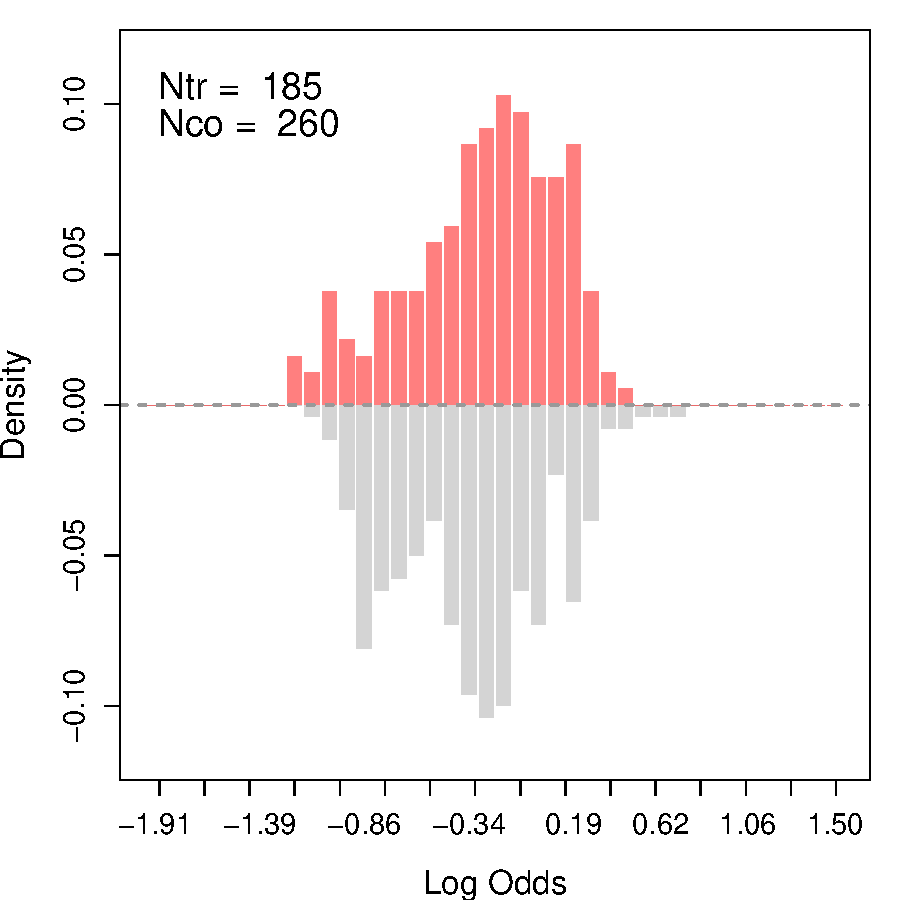
\includegraphics[width=\linewidth]{odds_ldw_exp.pdf}
            \caption{LDW-Experimental}
        \end{subfigure}
    \end{minipage}%
    % Second column
    \begin{minipage}[c]{.65\textwidth}
        \centering
        \begin{subfigure}{0.45\linewidth}
            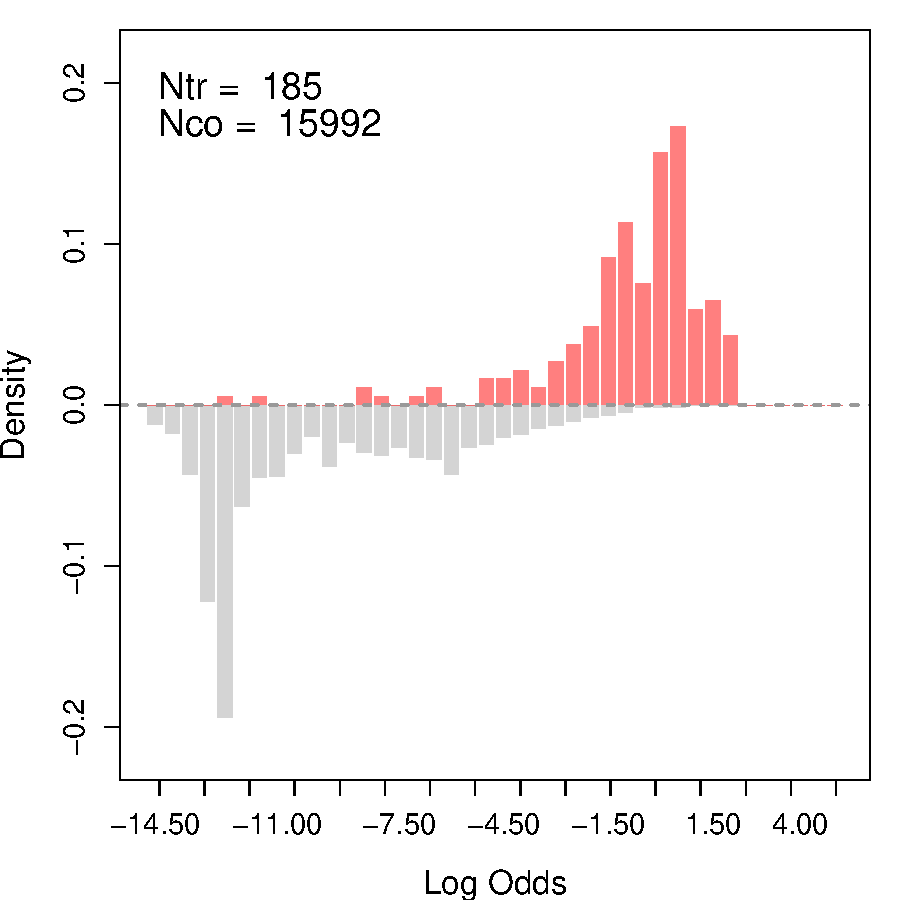
\includegraphics[width=\linewidth]{odds_ldw_cps.pdf}
            \caption{LDW-CPS}
        \end{subfigure}
        \begin{subfigure}{0.45\linewidth}
            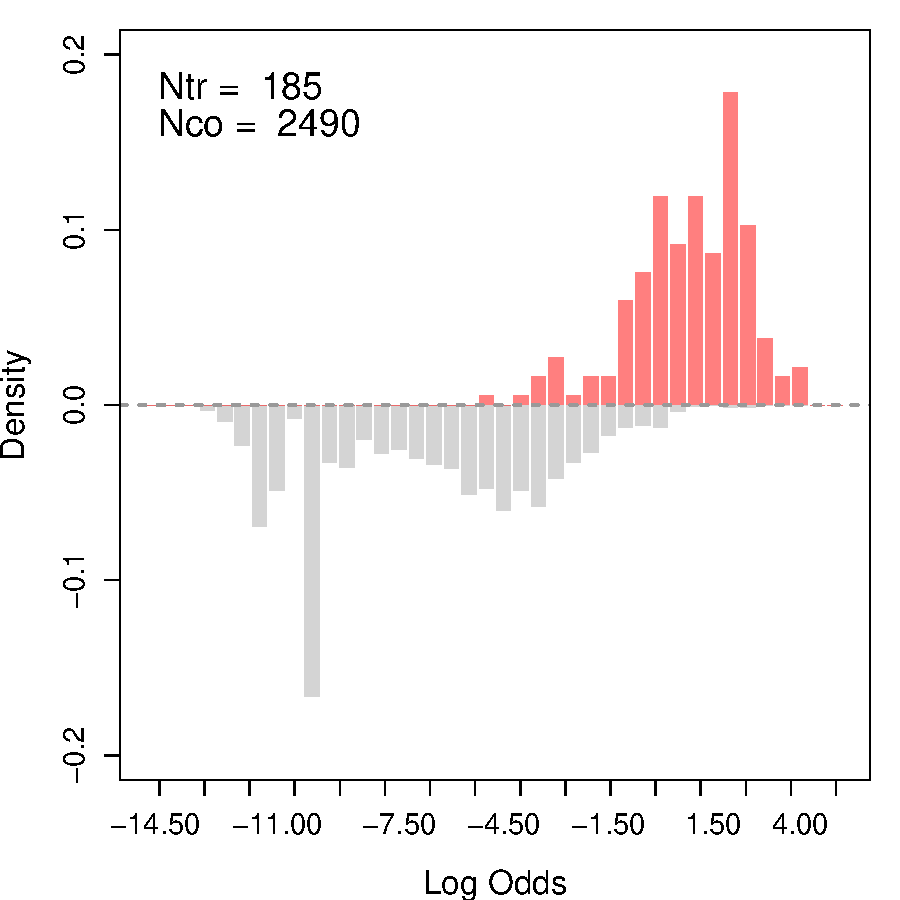
\includegraphics[width=\linewidth]{odds_ldw_psid.pdf}
            \caption{LDW-PSID}
        \end{subfigure}\\
        \begin{subfigure}{0.45\linewidth}
            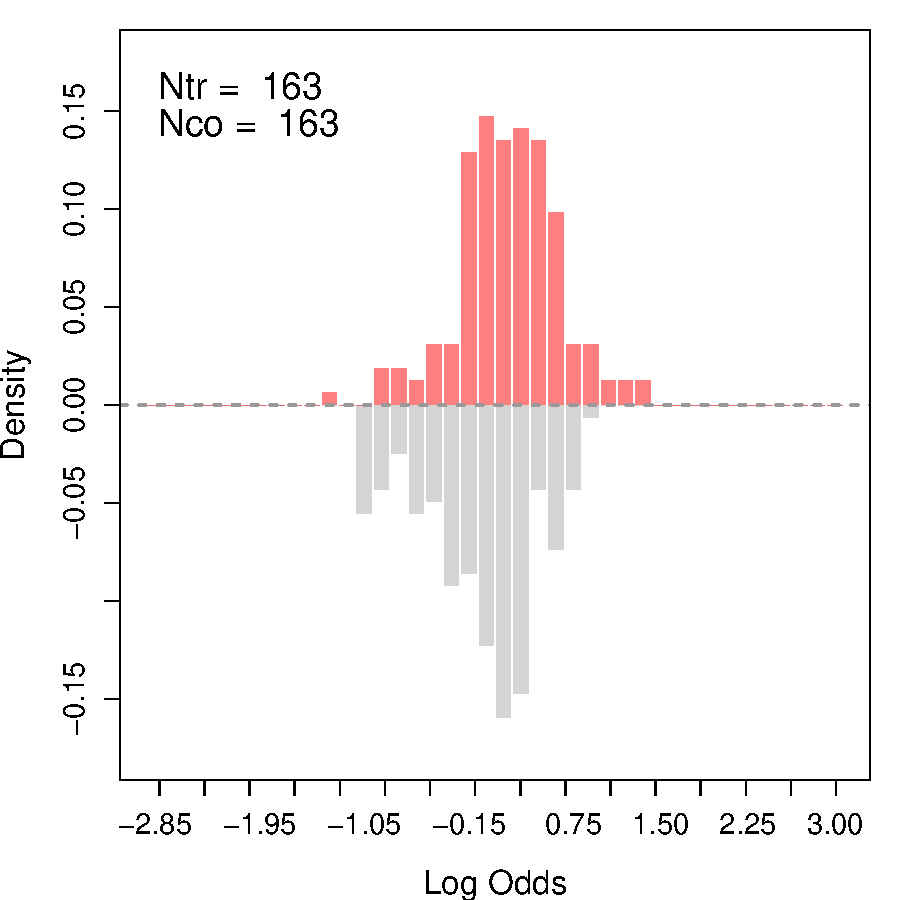
\includegraphics[width=\linewidth]{odds_ldw_cps_trim.pdf}
            \caption{Trimmed LDW-CPS}
        \end{subfigure}
        \begin{subfigure}{0.45\linewidth}
            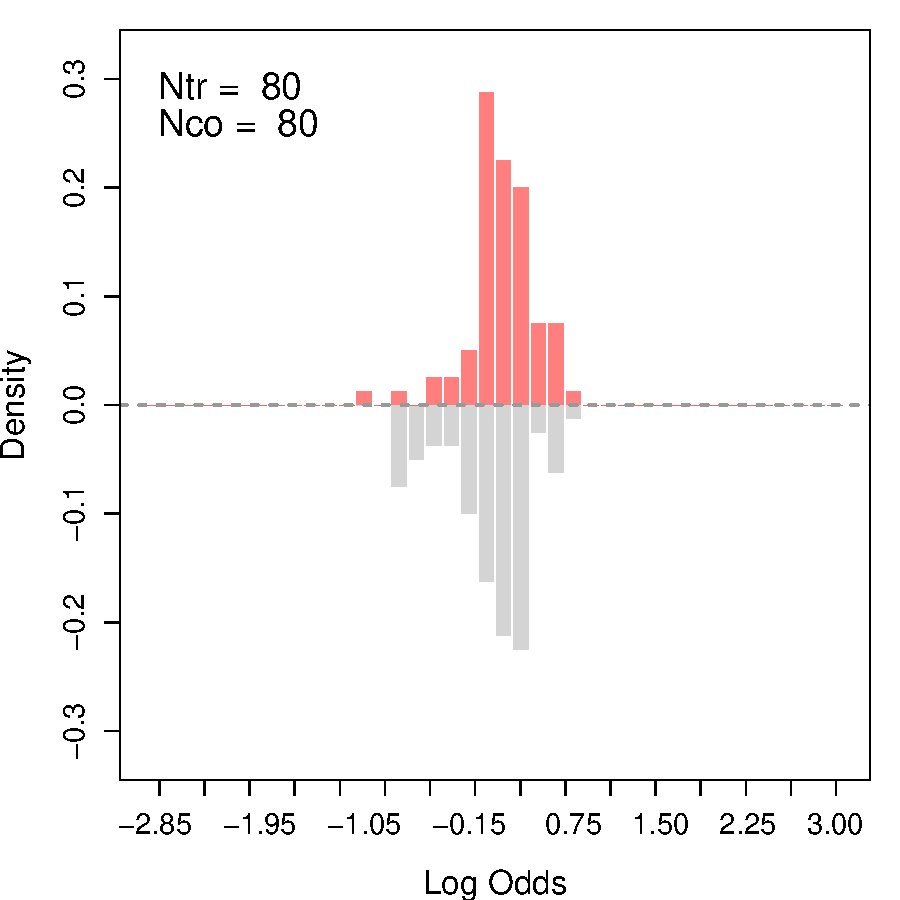
\includegraphics[width=\linewidth]{odds_ldw_psid_trim.pdf}
            \caption{Trimmed LDW-PSID}
        \end{subfigure}
    \end{minipage}%
    \\\raggedright
     {\footnotesize\textbf{\textit{Note:}} Histograms depict the log odds ratios, i.e., $\log\frac{\hat{e}}{1-\hat{e}}$, using propensity score estimated through GRF. Each subfigure represents a different sample. \textbf{Subfigure A}: LDW-Experimental. \textbf{Subfigure B}: LDW-CPS. \textbf{Subfigure C}: LDW-PSID. \textbf{Subfigure D}: Trimmed LDW-CPS. \textbf{Subfigure E}: Trimmed LDW-PSID. For C and D, the propensity scores are re-estimated after trimming.}
\end{figure}



\subsection{The LaLonde Data}

We primarily focus on the LDW data, give their inclusion of 1974 earnings and employment status. We use three LDW datasets: (1) LDW-Experimental, which consists of 185 treated and 280 control individuals from the experimental data; (2) LDW-CPS, including the same treated individuals and 15,992 controls from CPS-SSA-1; and (3) LDW-PSID, comprising the same treated individuals and 2,490 controls from PSID-1. We do not use CPS-SSA-2 and CPS-SSA-3 controls as they are subsets of CPS-SSA-1, and similarly, we do not use PSID-2 and PSID-3 as they are part of PSID-1. LaLonde's construction of these subsamples was a relatively {\it ad hoc} approach to improving overlap. We use more modern, fully data-driven ways to detect and address issues related to overlap.


Figure~\ref{fig:overlap} (A)-(C) display the overlaps in propensity score estimated from generalized random forest \citep[GRF,][]{athey2019generalized} between the treated and control units for all three samples, using histograms of the log-odds of propensity scores, {\it i.e.}, $\log\left(\hat{e}/(1-\hat{e})\right)$. As expected, LDW-Experimental shows almost perfect overlap. However, both nonexperimental samples show very poor overlaps. Most notably, the propensity scores of many treated units do not lie within the support of the controls' propensity scores, and a substantial proportion of the control units possess extremely low log odds. Similar patterns are observed with the original LaLonde male samples.

\paragraph{Trimming to improve overlap} Based on LDW-CPS and LDW-PSID, we further construct two trimmed samples to improve overlap. Trimming involves two steps. First, we merge the experimental controls from LDW-Experimental into LDW-CPS (or LDW-PSID) and estimate each unit's propensity of being included in the experiment using GRF.\footnote{In other words, both experimental treated units and controls are labeled as 1 and the nonexperimental units are labeled as 0. This approach is clearly not feasible when experimental controls are unavailable; our objective is to establish experimental benchmarks for the trimmed samples. We include the full set of covariates, including real earnings and unemployment status for the years 1974 and 1975.} 
\begin{figure}[!th]
\caption{Trimming the LDW Data}\label{fig:ldw.samples}
\vspace{-0.7em}
\begin{minipage}[c]{1\textwidth}
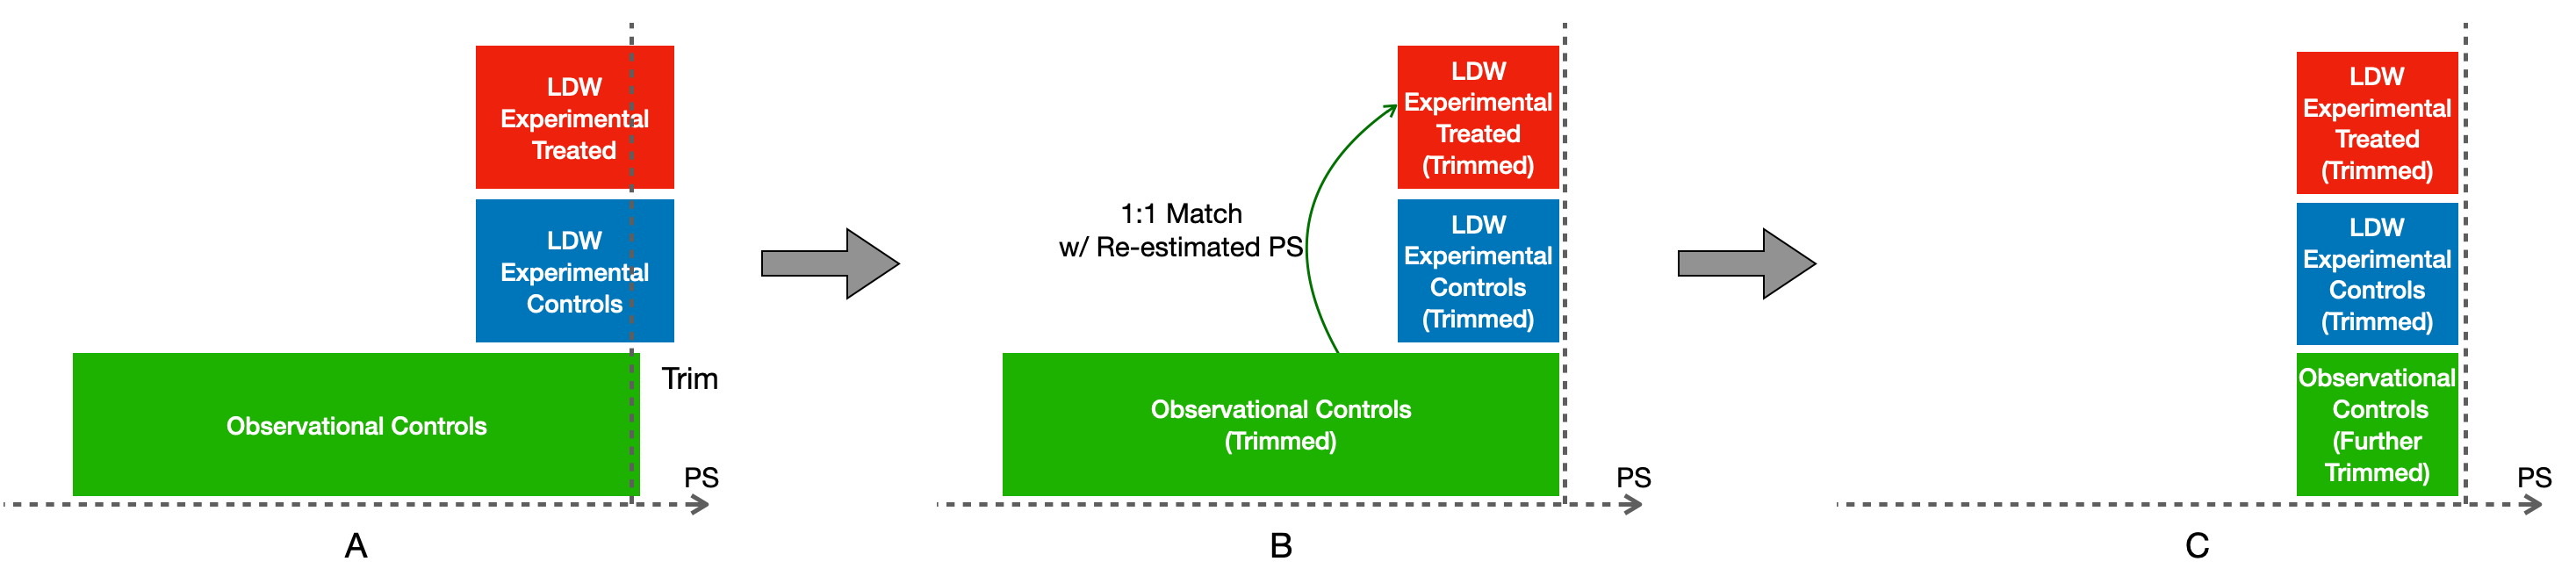
\includegraphics[width=\textwidth]{samples.png}
{\footnotesize\textbf{\textit{Note:}} A demonstration of the trimming procedure.}
\end{minipage}%
\end{figure}
We set a threshold to trim data with estimated propensity scores exceeding this value. The thresholds for LDW-CPS and LDW-PSID, chosen based on the numbers of available controls units, are 0.9 and 0.8, respectively.\footnote{Using CPS-SSA-1 as controls, only four control units have $\hat{e} > 0.9$; using PSID-1 as controls, only nine control units have $\hat{e} > 0.8$.} The transition from Step (A) to (B) in Figure~\ref{fig:ldw.samples} illustrates this step. We conduct this procedure to trim all three samples simultaneously to improve overlap in the final samples. This is because merely trimming the nonexperimental controls is inadequate, as the nonexperimental datasets lack particular profiles of participants of the experiment. For LDW-CPS, 22 treated units (12\%) are excluded, whereas for LDW-PSID, 105 treated units (57\%) are dropped. This underscores the large differences between the nonexperimental controls and the experiment participants based on covariate distributions.

Second, using the trimmed data and the same set of covariates, we re-estimate propensity scores using GRF, this time excluding the experimental controls. We then employ a 1:1 matching based on the re-estimated propensity scores to further trim the nonexperimental controls. This step is illustrated by the progression from Step (B) to (C) in Figure~\ref{fig:ldw.samples}. This procedure yields two samples: trimmed LDW-CPS (or trimmed LDW-PSID), composed of the trimmed experimental treated units and trimmed nonexperimental controls, and another trimmed experimental sample, consisting of trimmed experimental treated units and controls. The latter serves as an experimental benchmark for the former. As shown in Figure~\ref{fig:overlap}(D)-(E), overlap improves significantly in both samples post-trimming, though this comes with the cost of reduced sample sizes. We conduct similar procedures to the LaLonde male samples. 


%\FloatBarrier

\paragraph{Estimating the ATT} Next, we estimate the ATT using both the original LDW nonexperimental samples and the newly constructed trimmed samples. We apply a variety of estimators, including simple difference-in-means, regression, the Oaxaca Blinder estimator, GRF as an outcome model, nearest neighbor matching with bias correction, propensity score matching, IPW with propensity scores estimated by GRF, covariate balancing propensity score (CBPS), entropy balancing, double/debiased matching learning using elastic net, and AIPW implemented via GRF. All estimators use the same set of ten covariates as before. 



\begin{figure}[!ht]
    \caption{ATT Estimates Given Unconfoundedness: LDW Samples}\label{fig:ldw.att}
    \vspace{-1em}
    \begin{minipage}[c]{1\textwidth}
    \begin{center}
    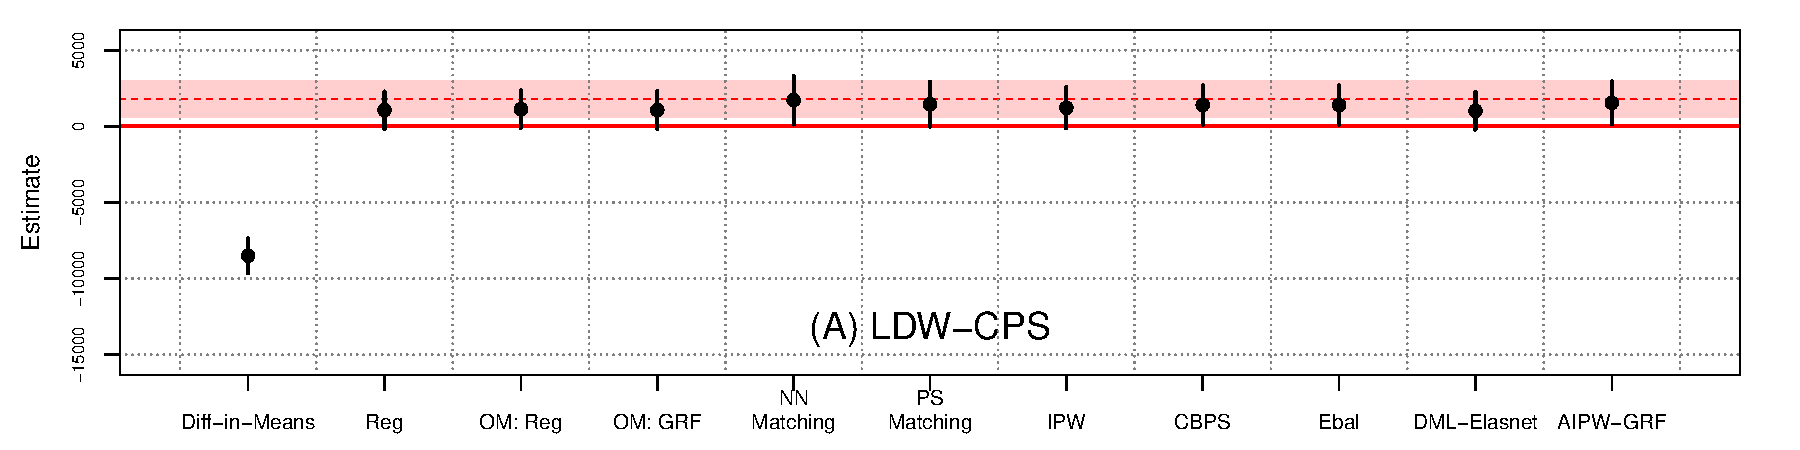
\includegraphics[width=0.8\linewidth]{coef_ldw_cps.pdf}
    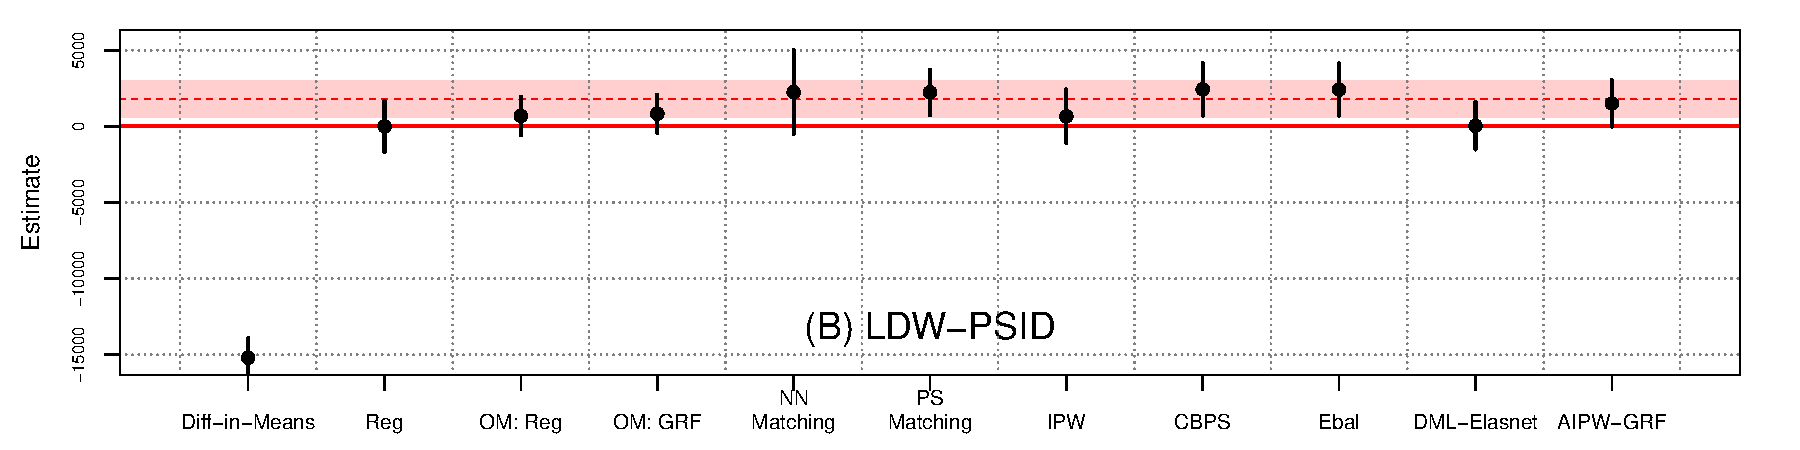
\includegraphics[width=0.8\linewidth]{coef_ldw_psid.pdf}
    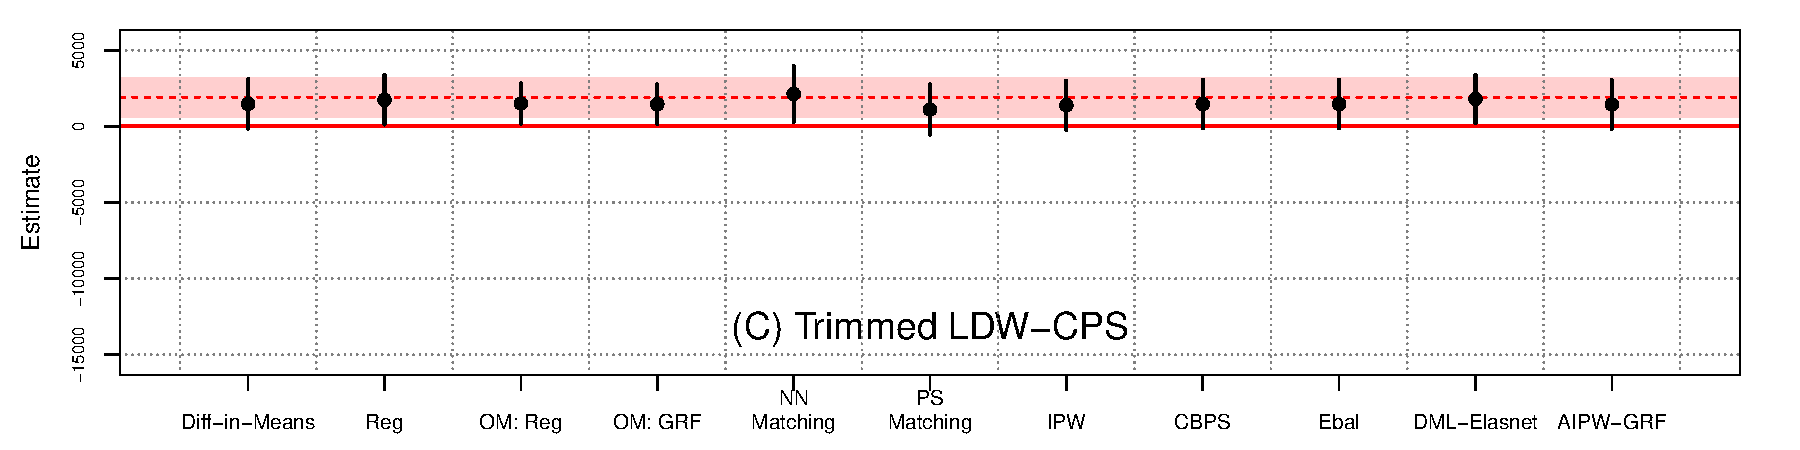
\includegraphics[width=0.8\linewidth]{coef_ldw_cps_trim.pdf}
    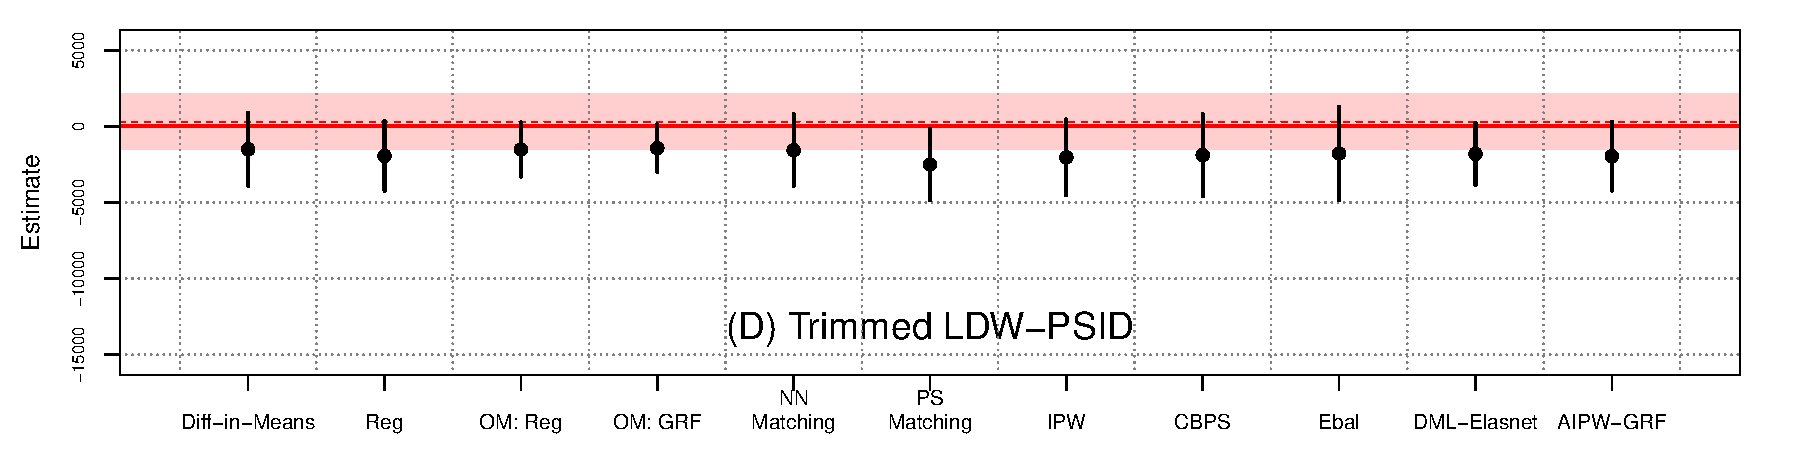
\includegraphics[width=0.8\linewidth]{coef_ldw_psid_trim.pdf}
    \end{center}    
     {\footnotesize\textbf{\textit{Note:}} The above figures show the ATT estimates and their 95\% confidence intervals using four different samples: LDW-CPS, LDW-PSID, Trimmed LDW-CPS, and Trimmed LDW-PSID. Eleven estimators are employed, including difference-in-means, linear regression, Oaxaca Blinder, GRF as an outcome model, 1: 5 nearest neighbor matching with bias correction, propensity score matching, IPW with propensity scores estimated by GRF, CBPS, entropy balancing, double/debiased matching learning with elastic net (implemented using \texttt{DoubleML}), and AIPW with GRF  (implemented using \texttt{grf}). The red dashed line and pink band represent the experiment benchmark and its 95\% confidence intervals, respectively.}
     \end{minipage}
\end{figure}

We present the findings in Figure~\ref{fig:ldw.att}, as well as Table~\ref{tb:ldw.est} in the SM. The first two panels present the ATT estimates and their 95\% confidence intervals from LDW-CPS and LDW-PSID, while the third and fourth panels show the results from the trimmed samples with improved overlap. In each figure, the ATT estimates using experimental data and their 95\% confidence intervals are highlighted with a red dashed line and pink band, respectively.

As shown in Figure~\ref{fig:ldw.att}(A), when using LDW-CPS, all estimators, except difference-in-means, produce positive estimates, although there are noticeable variations among them. Nearest neighbor matching outperforms other estimators, aligning closely with the experimental benchmark of \$1,794. Notably, CBPS, entropy balancing, and  AIPW-GRF also produce results close to the benchmark. Despite numerical differences, these estimates, except for difference-in-means, cannot be statistically distinguished from one another. Figure~\ref{fig:ldw.att}(B) shows that estimates based on LDW-PSID exhibit greater variations. Setting aside the difference-in-means, the estimates span from \$4 to \$2,420. Among them, the AIPW-GRF estimator produces an estimate closest to the experimental benchmark.

Figure~\ref{fig:ldw.att}(C) and (D) show that by using trimmed data with improved overlap, estimates produced by various estimators are substantially more stable. For trimmed LDW-CPS, all estimates hover around the experimental benchmark of \$1,911. This includes the simple difference-in-means estimator, which, due to trimming, is equivalent to propensity score matching without replacement. In the case of trimmed LDW-PSID, the experimental benchmark stands at \$306, and it is not statistically significantly different from zero at the 5\% level. While each estimator yields results that are closely aligned, they all have a negative sign. They are statistically indistinguishable from the experimental benchmark due to the large uncertainties associated with these estimates. The stability of the range of estimators after trimming is also found in the simulations in \citet{athey2021using}.

These findings suggest that while improved overlap based on observed covariates can reduce model dependency and estimate variability across different estimators, it does not guarantee consistency without validating unconfoundedness. The fact that many methods produce estimates that match the experimental benchmark for the ATT using LDW-CPS might have instilled unwarranted confidence in researchers that modern estimators can help achieve causal identification even when there are no compelling reasons to believe unconfoundedness. In other words, while modern methods may be effective in estimating the statistical estimand, the  covariate-adjusted difference between the treated and control outcomes, that does {\it not} mean that this adjusted difference is close to the ATT. For that, we need some version of the unconfoundedness assumption, which is untestable.

\FloatBarrier

\paragraph{Alternative estimands: CATT and quantile treatment effects} Exploring causal estimates for alternative estimands, such as heterogeneous treatment effects and quantile treatment effects, can shed light on the plausibility of unconfoundedness. Using both the original LDW data and the trimmed versions, we estimate the CATT using a causal forest through AIPW-GRF. In Figure~\ref{fig:catt}, we plot the estimated CATT from nonexperimental data at the covariate values of each treated unit against their corresponding experimental benchmarks. Each of the four panels uses a different dataset. Every gray dot represents a pair of CATT estimates, while the red cross depicts the pair of estimated ATTs, also estimated via AIPW-GRF. This exercise is, in essence, similar to the test proposed by \cite{atheyimbens_robust} to explore a finding's robustness to model specifications by splitting samples based on covariate values.

\begin{figure}[!ht]
    \caption{CATT Estimates using LDW Data: Experimental vs. Nonexperimental}\label{fig:catt}
    \centering
    \begin{minipage}[c]{1\textwidth}
        \centering
        \begin{subfigure}{0.45\linewidth}
            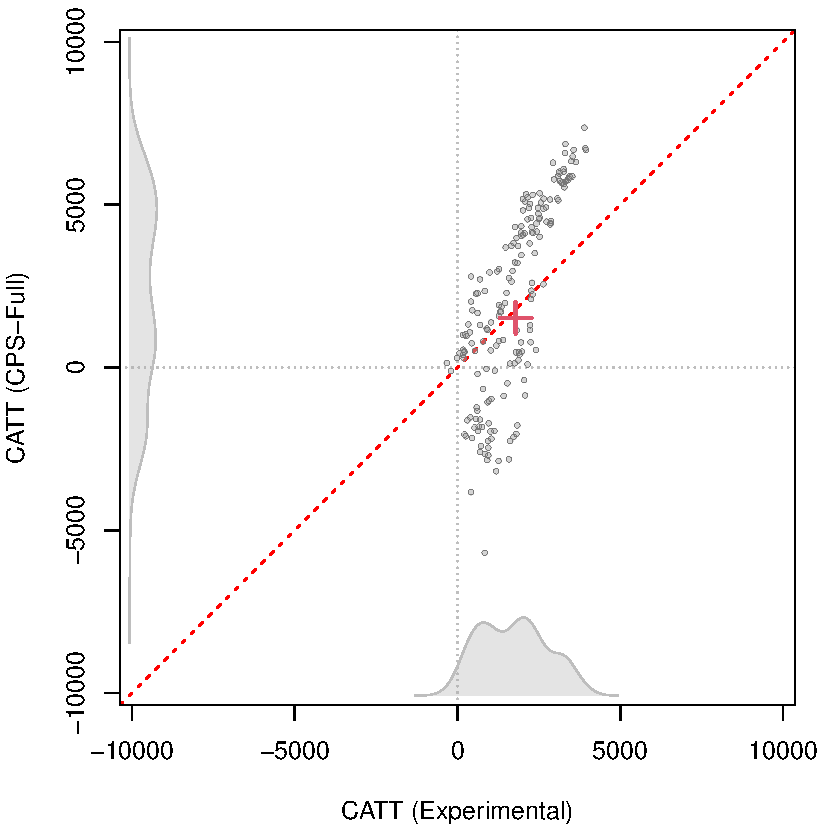
\includegraphics[width=\linewidth]{catt_cps.pdf}
            \caption{LDW-CPS}
        \end{subfigure}
        \begin{subfigure}{0.45\linewidth}
            \includegraphics[width=\linewidth]{catt_PSID.pdf}
            \caption{LDW-PSID}
        \end{subfigure}\\
        \begin{subfigure}{0.45\linewidth}
            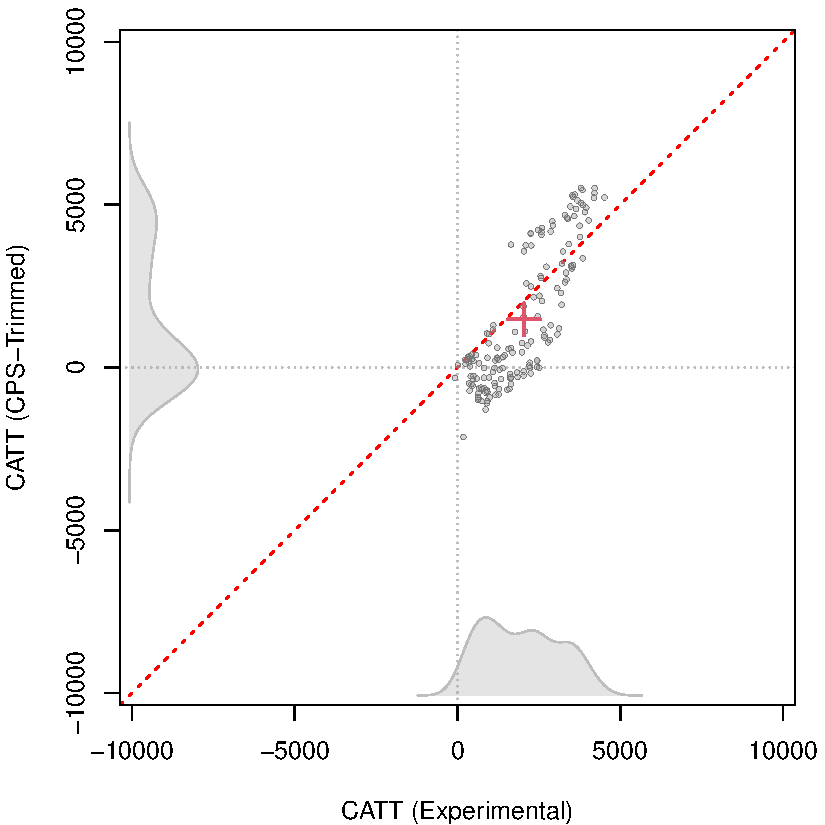
\includegraphics[width=\linewidth]{catt_cps_trim.pdf}
            \caption{LDW-CPS Trimmed}
        \end{subfigure}
        \begin{subfigure}{0.45\linewidth}
            \includegraphics[width=\linewidth]{catt_PSID_trim.pdf}
            \caption{LDW-PSID Trimmed}
        \end{subfigure}
    \end{minipage}%
    \\\raggedright
     {\footnotesize\textbf{\textit{Note:}} Scatterplots show the CATT using both experimental data (x-axis) and nonexperimental data (y-axis). Each dot corresponds to a CATT estimate based on the covariate values of a treated unit, while each red cross symbolizes the ATT estimates. For every estimate, the AIPW estimator is employed, with the GRF approach for estimating nuisance parameters. Different subfigures indicate various data comparisons: \textbf{Subfigure A}: Compares LDW-Experimental with LDW-CPS. \textbf{Subfigure B}: Compares LDW-Experimental with LDW-PSID. \textbf{Subfigure C}: Compares trimmed LDW-Experimental (removing 22 treated units) against trimmed LDW-CPS. \textbf{Subfigure D}: Compares trimmed LDW-Experimental (removing 70 treated units) to trimmed LDW-PSID.}
\end{figure}

Figure~\ref{fig:catt} shows that although the AIPW estimator can produce ATT estimates closely aligned with the experimental benchmark using LDW data, its performance for revealing the true CATT is considerably worse. Specifically, with LDW-CPS, CATT estimates span from \$-5,693 to \$7,364, contrasting with the CATT estimated from experimental data which ranges from \$-329 to \$3,946. It overestimates CATT that exceed the ATT and underestimates CATT that fall below the ATT. Employing LDW-PSID generates CATT estimates ranging from \$-8874 to \$4701. With trimmed LDW-CPS, the CATT estimates align more closely with those from the experimental data. However, using trimmed LDW-PSID, the majority of CATT estimates are negative, suggesting significant biases.

\begin{figure}[!ht]
    \caption{Quantile Treatment Effects: Experimental vs. Nonexperimental}\label{fig:ldw.qte}
    \begin{minipage}[c]{1\textwidth}
        \centering\vspace{-1em}
        \begin{subfigure}{1\linewidth}\hspace{1em}\centering
            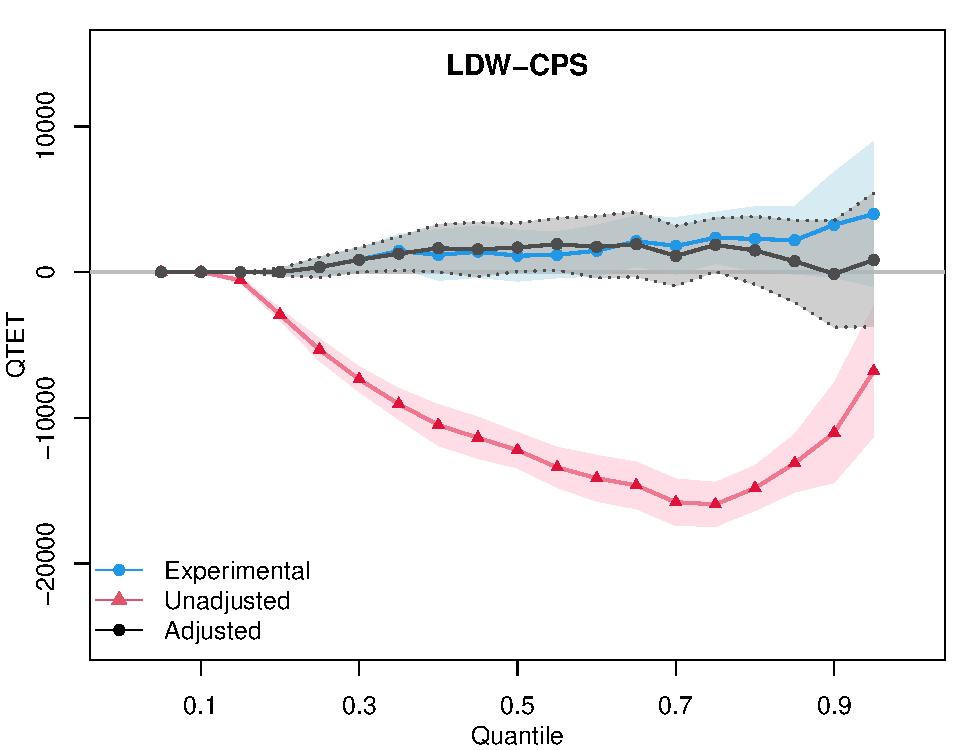
\includegraphics[width=0.45\linewidth]{qte_ldw_cps.pdf}\hspace{2em}
            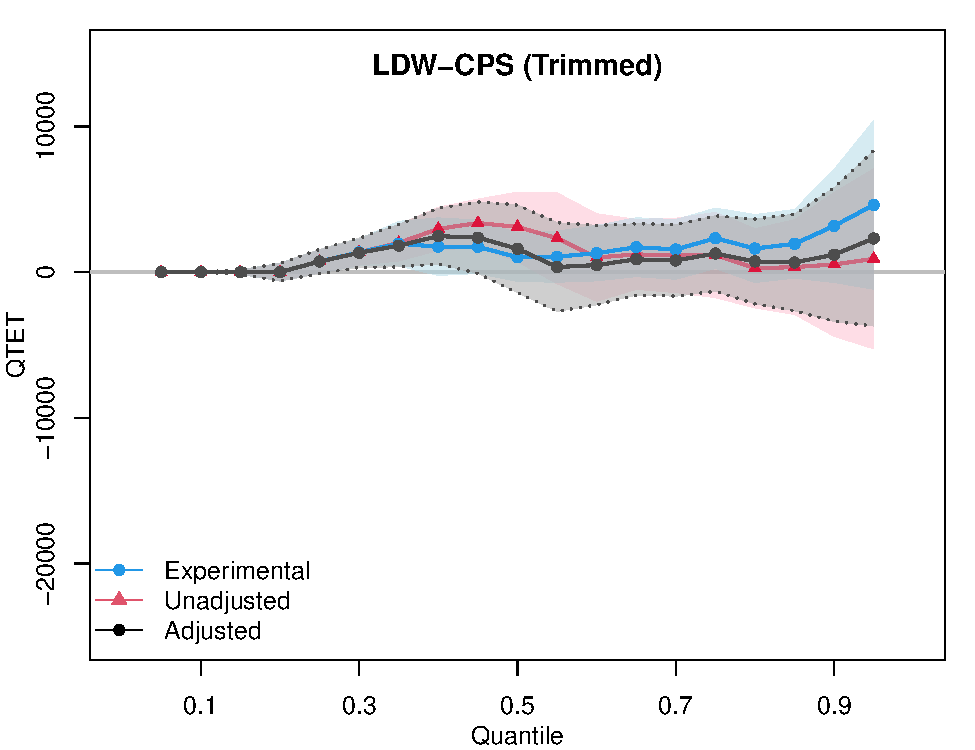
\includegraphics[width=0.45\linewidth]{qte_ldw_cps_trim.pdf}
            \caption{LDW-CPS}
        \end{subfigure}\\
        \begin{subfigure}{1\linewidth}\hspace{1em}\centering
            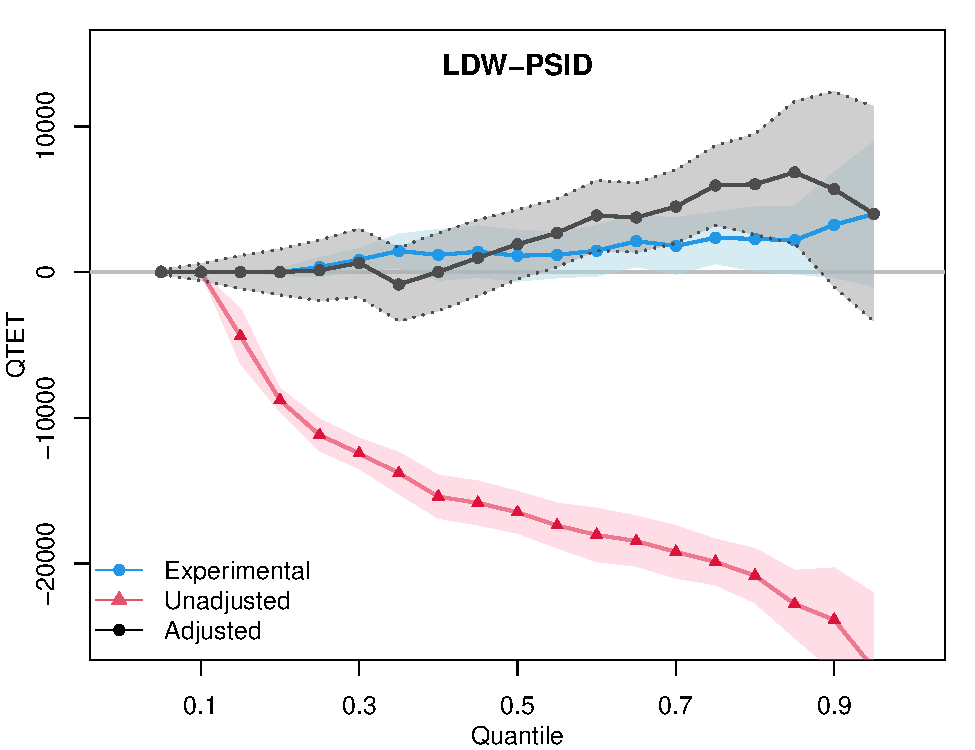
\includegraphics[width=0.45\linewidth]{qte_ldw_psid.pdf}\hspace{2em}
            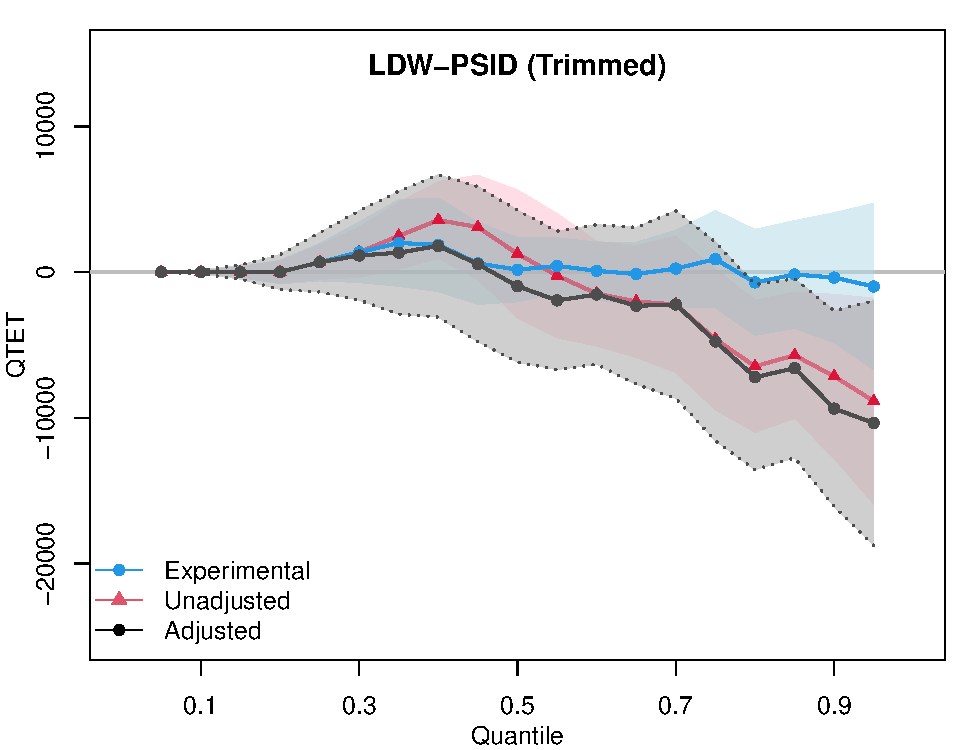
\includegraphics[width=0.45\linewidth]{qte_ldw_psid_trim.pdf}
            \caption{LDW-PSID}
        \end{subfigure}
    \end{minipage}%
    \\\raggedright
     {\footnotesize\textbf{\textit{Note:}} Figures show the quantile treatment effects on the treated (QTET) using both experimental data (in blue) and nonexperimental data (in red for raw estimates and black for covariate-adjusted estimates). Each dot corresponds to a QTET estimate at a particular quantile, while shaded areas represent bootstrapped 95\% confidence intervals. Unadjusted models do not incorporate covariates while adjustment models use the full set of covariates to estimate the propensity scores with a logit. \textbf{Subfigure A}: Compares LDW experimental data with LDW-CPS. \textbf{Subfigure B}: Compares LDW experimental data with LDW-PSID.}
\end{figure}

We estimate the quantile treatment effects on the treated (QTET) using an IPW approach proposed by \citet{firpo2007efficient}. Figure~\ref{fig:ldw.qte} plots the QTET estimates using both the LDW experimental data and nonexperimental data.  The QTET estimates from either the original or trimmed LDW-CPS data align reasonably well with the true QTET, although they are often underpowered. On the other hand, using LDW-PSID data, be it original or trimmed, the estimated QTET display notable biases when compared to the experimental benchmark, which is close to zero.

These exercises suggest that, when considering alternative estimands such as CATT and QTET, among the four nonexperimental samples, overall, only trimmed LDW-CPS produces results consistently aligned closely with the experimental benchmarks.

%\FloatBarrier


\paragraph{Validation through placebo analyses} We conduct placebo analyses to further assess how plausible unconfoundedness is. To do so, we select earnings in 1975 (\texttt{re75}) as the placebo outcome and remove both \texttt{re75} and \texttt{u75} from the set of conditioning variables. Two new trimmed samples are created without using \texttt{re75} and \texttt{u75}. We then estimate the ATT for the placebo outcome, conditional on the remaining covariates, using a variety of estimators. Figure~\ref{fig:ldw.placebo} presents the findings. Not surprisingly, the experimental benchmarks are near zero and statistically insignificant. However, all estimators using nonexperimental data generate large, negative estimates. Again, with trimmed data, the estimates are stable but remain statistically different from zero. Moreover, Figure~\ref{fig:ldw.catt.placebo} in the SM further shows that while the CATT estimates from the experimental data hover close to zero, their nonexperimental counterparts are all negative and substantial in magnitude, indicating large biases.

\begin{figure}[!ht]
    \caption{Placebo Tests: '75 Earnings as the Outcome}\label{fig:ldw.placebo}
    \vspace{-1em}
    \begin{minipage}[c]{1\textwidth}
    \begin{center}
    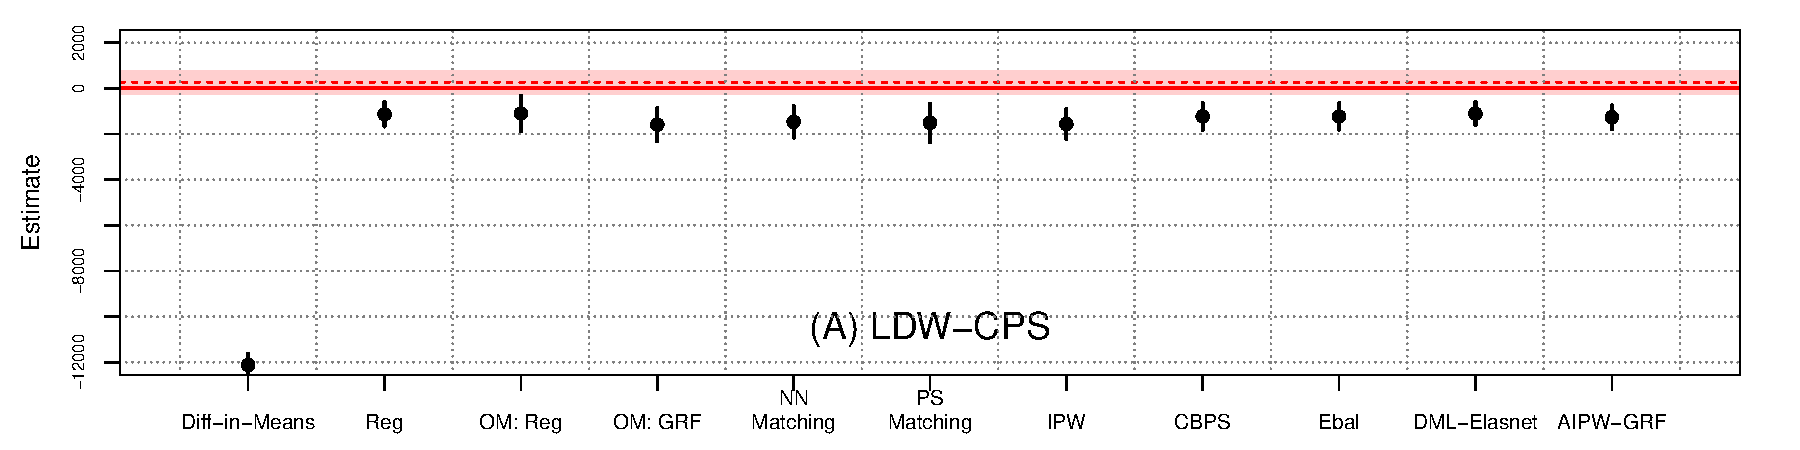
\includegraphics[width=0.8\linewidth]{coef_ldwp_cps.pdf}
    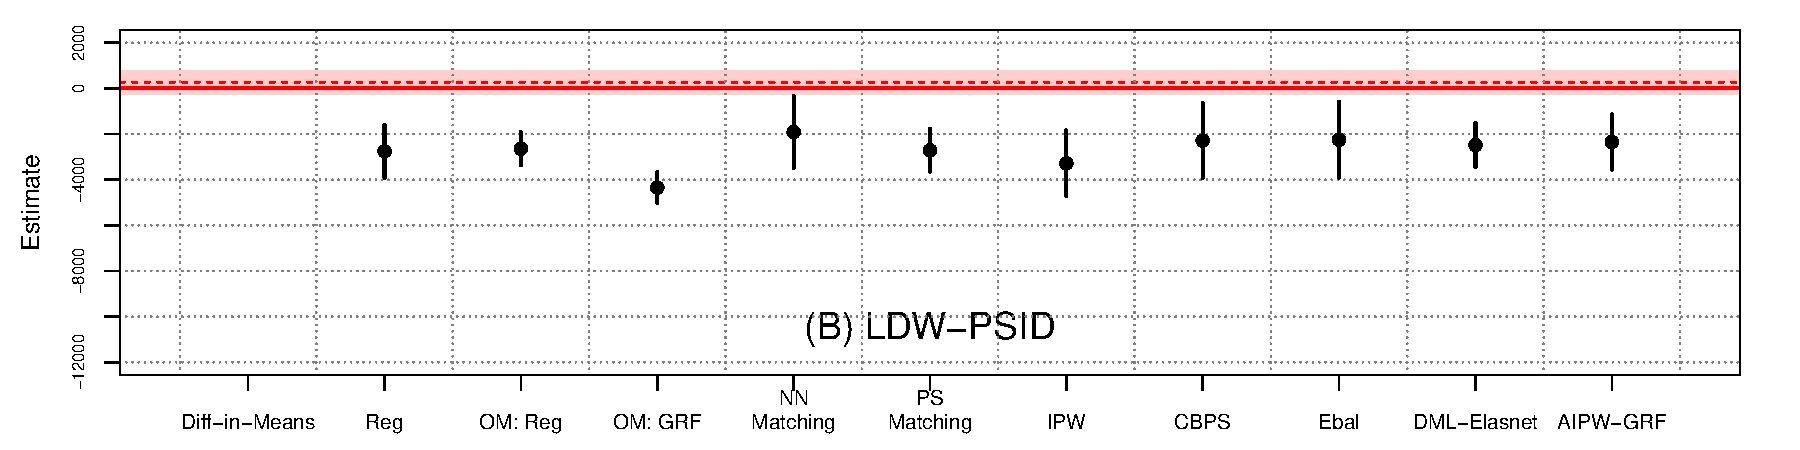
\includegraphics[width=0.8\linewidth]{coef_ldwp_psid.pdf}
    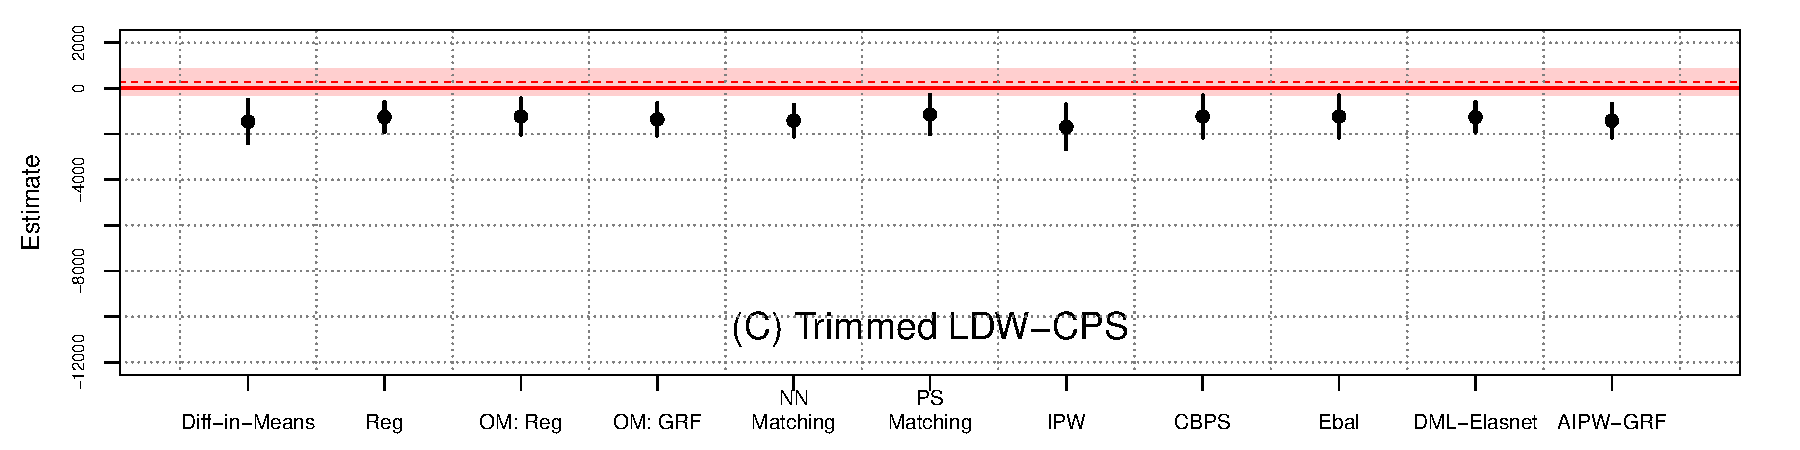
\includegraphics[width=0.8\linewidth]{coef_ldwp_cps_trim.pdf}
    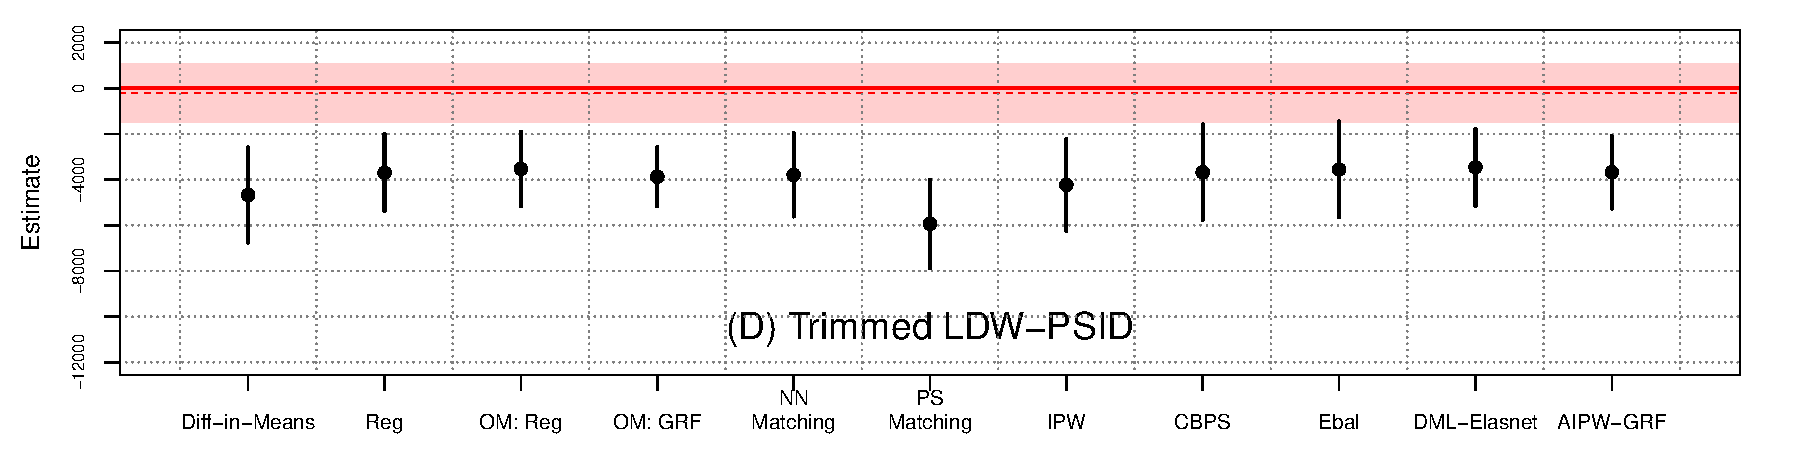
\includegraphics[width=0.8\linewidth]{coef_ldwp_psid_trim.pdf}
    \end{center}    
     {\footnotesize\textbf{\textit{Note:}} The above figures show the placebo estimates and their 95\% confidence intervals using four different samples: LDW-CPS, Trimmed LDW-CPS, LDW-PSID, and Trimmed LDW-PSID. We use the same eleven estimators as before. The red dashed line and pink band represent the experiment benchmark and its 95\% confidence intervals, respectively. The difference-in-means estimate for LDW-PSID is -17,531, which is not shown because it exceeds the y-axis range.}
     \end{minipage}
\end{figure}

\paragraph{Sensitivity analyses} We also conduct sensitivity analyses using the LDW data, with results depicted in contour plots in Figure~\ref{fig:ldw.sens} in the SM. The analyses suggest that the estimated training effect based on trimmed LDW-CPS is less sensitive to potential confounders compared to trimmed LDW-PSID. For instance, with trimmed LDW-CPS, the estimate remains positive and large even when a confounder's correlations with treatment and outcome are triple those of \texttt{re75}, whereas the presence of a confounder similar to \texttt{re75} would lead to a negative estimated effect using trimmed LDW-PSID.

\paragraph{The original LaLonde male samples} For comparison, we also revisit the original male samples used in \citet{LaLonde}. Table~\ref{tb:nsw.est} in the SM reports the ATT estimates using the original LaLonde male samples, of which the LDW sample is a subset. Two covariates, \texttt{re74} and \texttt{u74}, are absent from this sample. It shows that, with sufficient overlap, most modern estimators yield estimates within relatively narrow ranges when using either CPS-SSA-1 or PSID-1 as control groups. However, these estimates do not align with the experimental benchmarks, with most estimates being negative. \citet{smith2001reconciling, smith2005does} report similar, negative findings. 

\paragraph{The reconstructed AFDC female samples} Using the LCS female samples, we find that many modern methods yield estimates close to the experimental benchmarks, though standard errors are often quite large. While selection appears to be less severe for AFDC women compared to the male NSW participants, as suggested by \citet{calonico2017women}, overlap remains a significant challenge. Additionally, we fail to substantiate the unconfoundedness assumption with a placebo test using the number of children in 1975, a variable absent in \citet{LaLonde}, as the placebo outcome.   

\paragraph{Summary} After reexamining the LaLonde data, we offer some new insights into the challenge posed by \citet{LaLonde}. First, we agree with existing literature that ensuring overlap and using comparable control units are essential for credible causal estimates. Second, while the choice of method is less critical with overlap, as most methods yield similar results, the propensity score remains a vital tool for assessing overlap and is integral to many estimators. Third, we stress the importance of understanding the treatment assignment mechanism and the need for additional tests to validate unconfoundedness. With the LDW and LCS data, many methods approximate the experimental benchmark for the \emph{average effects} under overlap, a success not mirrored with the original LaLonde male samples. However, even with LDW or LCS data, placebo tests fail to substantiate unconfoundedness, and sensitivity analysis reveals the fragility of the regression estimate using either LDW-PSID or LCS-PSID.


%\FloatBarrier




\FloatBarrier

\subsection{Lottery Prizes on Labor Earnings}\label{re:irs}

We now reanalyze the lottery data from \citet*{imbensrubinsacerdote}, who carried out an original survey to investigate the impact of the size of lottery prizes in Massachusetts during the mid-1980s on the economic behavior of lottery players. The primary outcome is post-winning labor earnings. This empirical example is appealing for two reasons: (1) we have a much better understanding of the treatment assignment process (lottery), and (2) six periods of lagged outcomes are available to validate the unconfoundedness assumption.

There are three treatment and control groups. The control group, termed ``non-winners,'' consists of 259 season ticket holders who have won a small, one-time prize, ranging from \$100 to \$5,000 (in essence, they are one-time, minor winners). The treatment groups, labeled ``big winners'' (43 individuals) and ``small winners'' (194 individuals), are those who clinched a major prize. They might be season ticket holders or one-time buyers. The annual installments for these prizes ranged from \$1,139 to \$99,888 and exceeded \$100,000, respectively. These prizes were disbursed in yearly installments for over 20 years. 

While randomization should ideally ensure that the treatment and control groups are comparable at the time of the lottery entry, the authors highlight three potential reasons this might not be the case. First, individuals can purchase multiple tickets, increasing their odds of winning. Second, those who hold season tickets might differ from those who buy single tickets. Lastly, there were discrepancies in the response rates between winners and non-winners (49\% and 42\%, respectively), and these response rates could be influenced by a range of factors. However, the authors expect that the unconfoundedness assumption will hold once they condition on a set of observable covariates, including the year of winning and the number of tickets bought. Importantly, they also gathered data on past labor earnings for up to six years before the individuals won a prize. These past outcomes can be utilized either as conditioning variables or as placebo outcomes.

\begin{figure}[!ht]
    \caption{Assessing Overlap in IRS Data}\label{fig:irs.overlap}
    \centering
    \vspace{-0.5em}
    \begin{minipage}[c]{.9\linewidth}
        \centering
        \hspace{-2em}\begin{subfigure}{0.45\linewidth}
            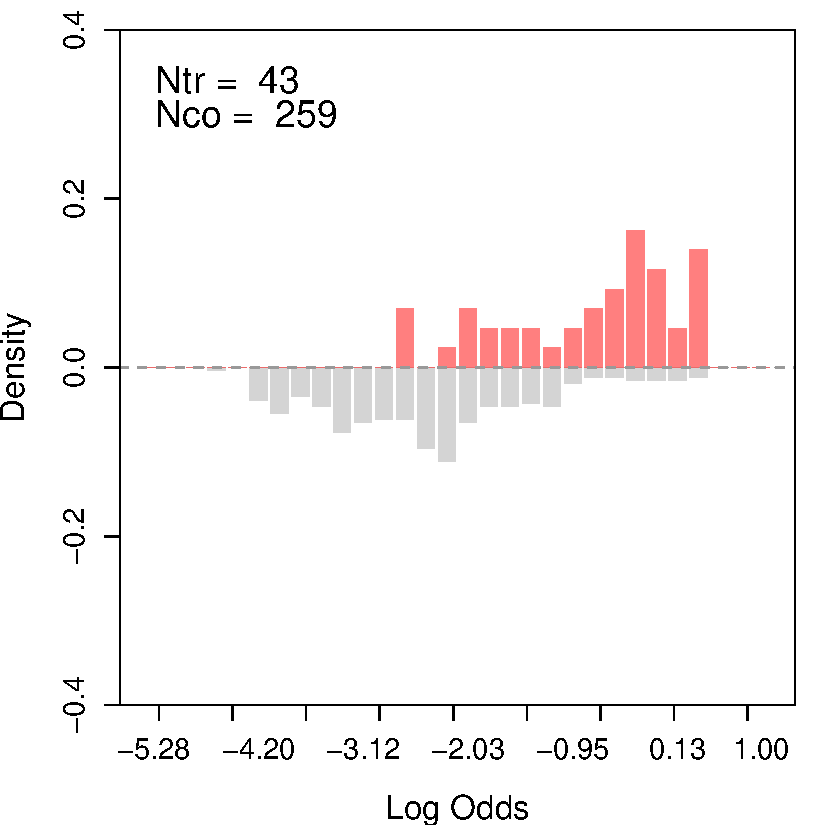
\includegraphics[width=\linewidth]{irs1_odds.pdf}
            \caption{Big Winners vs Non-Winners}
        \end{subfigure}\hspace{1em}
        \begin{subfigure}{0.45\linewidth}
            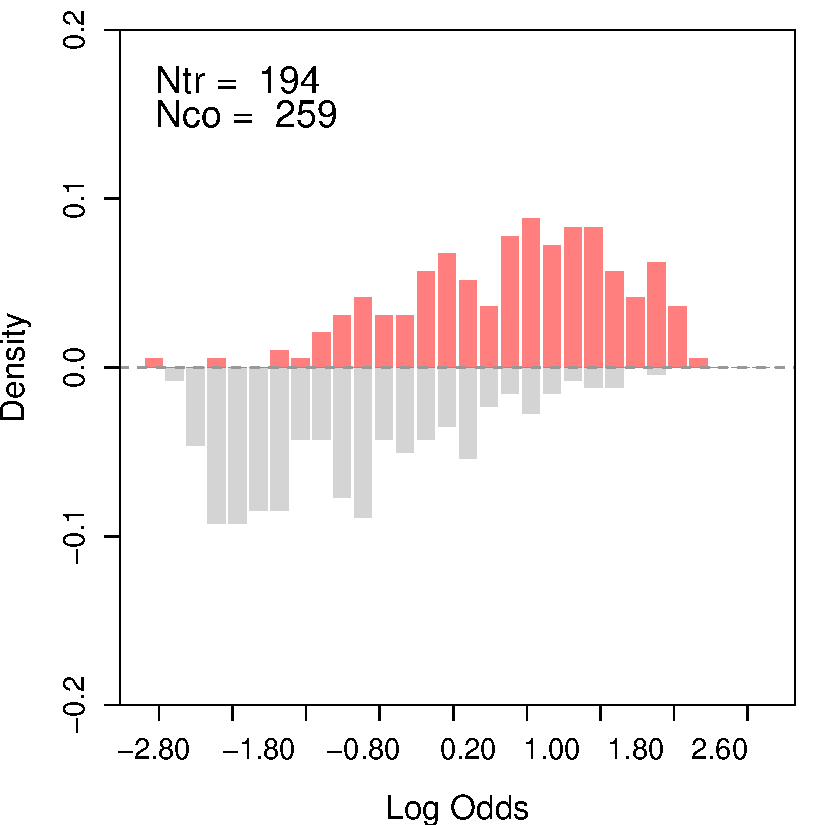
\includegraphics[width=\linewidth]{irs2_odds.pdf}
            \caption{Small Winners vs Non-Winners}
        \end{subfigure}
    \end{minipage}%
    \\\raggedright
     {\footnotesize\textbf{\textit{Note:}} Histograms depict the log odds ratios, i.e., $\log\frac{\hat{e}}{1-\hat{e}}$, using propensity scores estimated through GRF. }
\end{figure}


In the subsequent analysis, we will consider labor earnings from seven post-lottery-winning periods as the outcomes. These are denoted as $Y_{i, 0}, ..., Y_{i, 6}$, where $t=0$ represents the year of winning a lottery---recall that individuals in the control group also received a modest, one-time prize that year. We will treat the labor earnings from the three years immediately preceding the lottery win, i.e., $Y_{i,-3}, Y_{i,-2}, Y_{i,-1}$, as well as their average, as placebo outcomes. The labor earnings from the three years before those, i.e., $Y_{i,-6}, Y_{i,-5}, Y_{i,-4}$, will be used as covariates for adjustment, alongside a set of time-invariant pre-lottery-winning variables. These include the number of tickets purchased (\texttt{tixbot}), gender (\texttt{male}), employment status at the time of winning (\texttt{workthen}), age when the lottery was won (\texttt{agew}), total years of education (\texttt{educ}), and the presence of a college degree (\texttt{college}). Figure~\ref{fig:irs.overlap} assesses the overlap between the two treatment groups and the control group using the mentioned covariates. The figure indicates that while the propensity score distribution of individuals in the treatment groups differ from that of the control group, the propensity scores of the treatment groups still fall within the support of the control group.\footnote{To improve overlap, we further trim the control group for each of the two treatment groups by implementing 1:1 matching based on propensity scores, resulting in two trimmed samples. As shown in the SM, the results based on the trimmed samples are very similar to those based on the original data.}

\begin{figure}[!ht]
    \caption{ATT and Placebo Estimates: IRS Data}\label{fg:irs.est}
    \vspace{-1em}
    \begin{minipage}[c]{1\textwidth}
    \begin{center}
    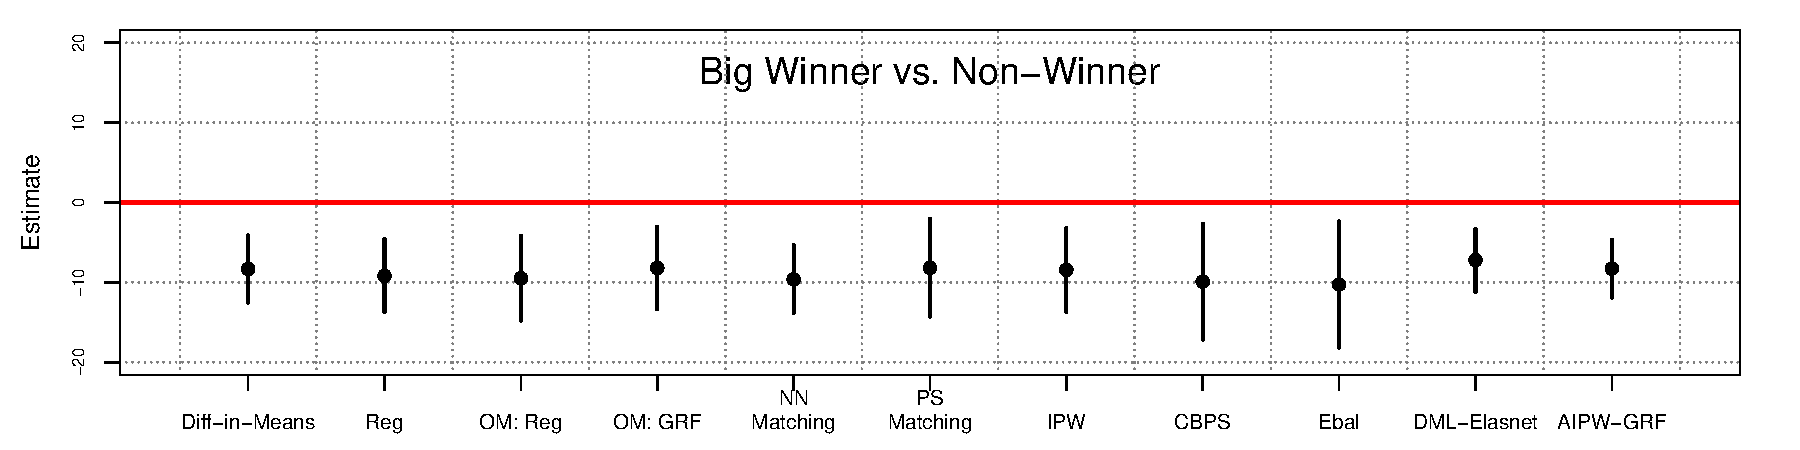
\includegraphics[width=0.8\linewidth]{irs_coef_big.pdf}
    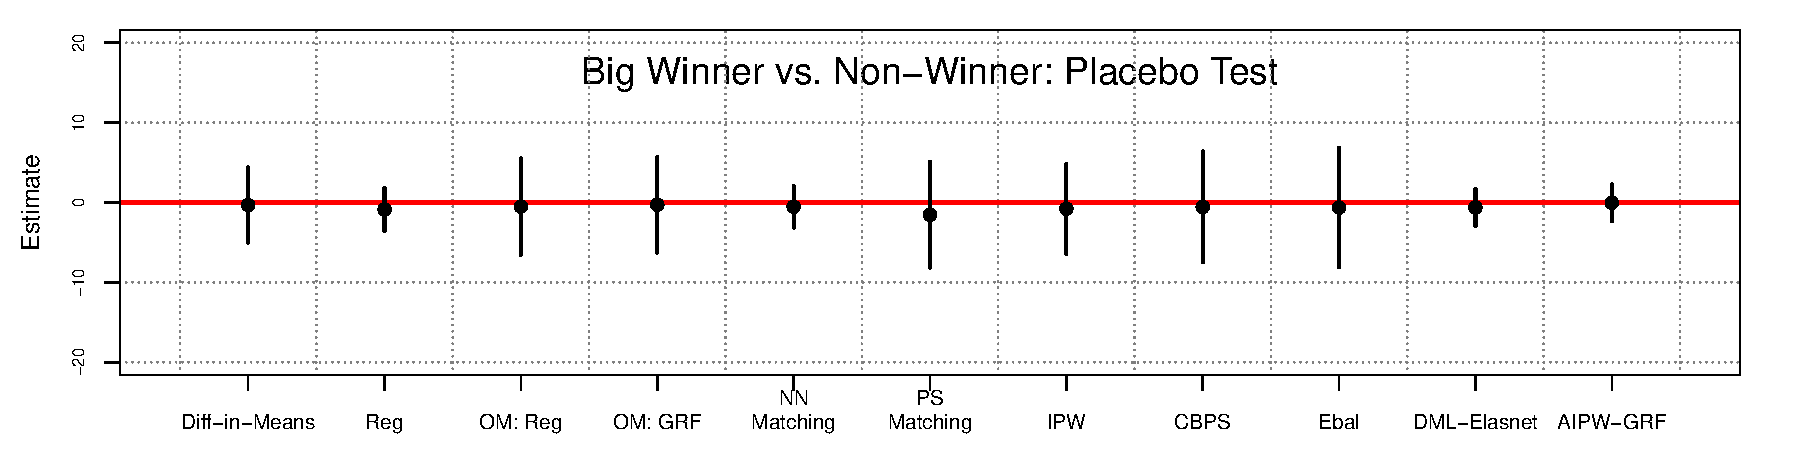
\includegraphics[width=0.8\linewidth]{irs_coef_big_pl.pdf}
    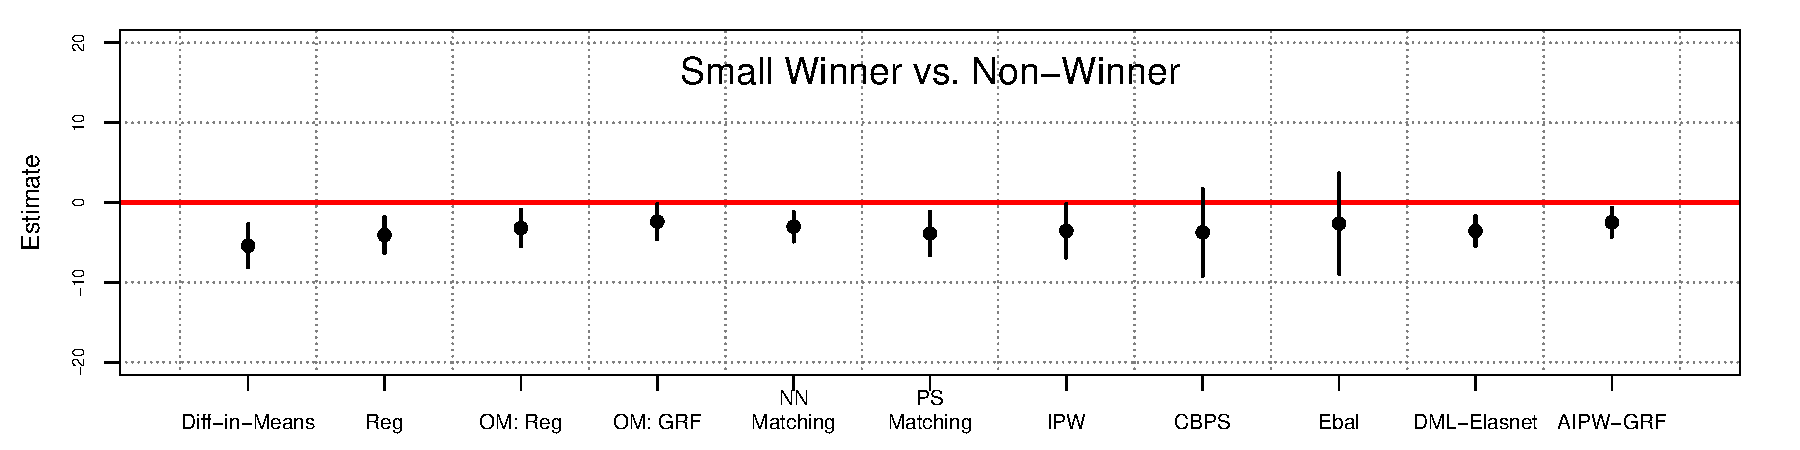
\includegraphics[width=0.8\linewidth]{irs_coef_small.pdf}
    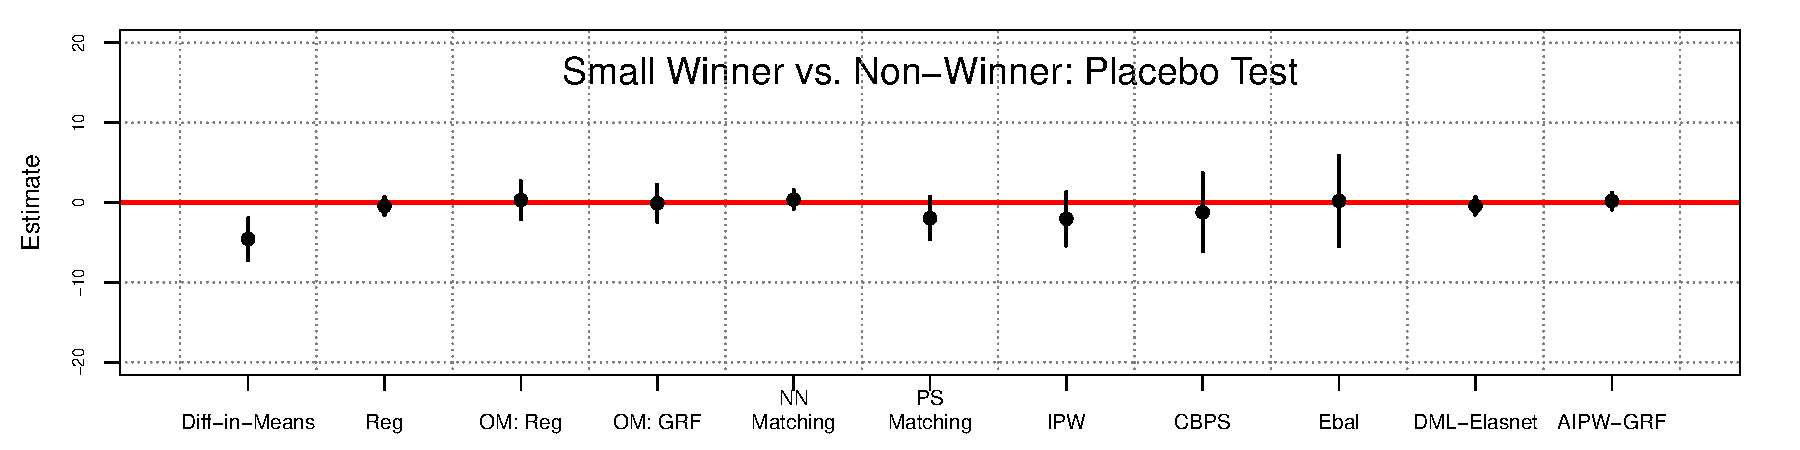
\includegraphics[width=0.8\linewidth]{irs_coef_small_pl.pdf}
    \end{center}    
     {\footnotesize\textbf{\textit{Note:}} Subfigure (A) and (C) show the ATT estimates of big and small winners, respectively, versus non-winners on the average annual labor earnings from Year 0 to Year 6, along with their 95\% confidence intervals. Subfigure (B) and (D) show the ATT estimates of big and smaller winners, respectively, versus non-winners on the placebo outcome, the average annual labor earnings from Year –3 to Year –1, along with their 95\% confidence intervals. We use the same eleven estimators as before. }
     \end{minipage}
\end{figure}

Figure~\ref{fg:irs.est} plots the ATT estimates, using various estimators, of the effect of lottery prizes on the real outcome (the average annual labor earnings from Year $0$ to Year $6$) and the placebo outcome (the average annual labor earnings from Year $-3$ to Year $-1$). The first two panels compare ``big winners'' with ``non-winners,'' while the third and fourth panels compare ``small winners'' with ``non-winners.'' Figure~\ref{fg:irs.est} shows that various covariate adjustment methods produce consistent results, which align with the findings reported in the original paper: winning a large prize leads to a significant decrease in labor income in the following years, averaging as much as \$8,000 annually. In contrast, winning a smaller prize results in a more modest decline, averaging approximately \$3,000 per year. When doubly robust estimators (such as AIPW-GRF) are employed, the estimates for the placebo effects are very close to zero, lending support to the unconfoundedness assumption.

\begin{figure}[!ht]
    \caption{ATT and CATT Estimates: IRS Data}\label{fig:irs.est}
    \centering\vspace{-0.5em}
    \begin{minipage}[c]{1\textwidth}
        \centering
        \hspace{-2em}\begin{subfigure}{0.45\linewidth}
            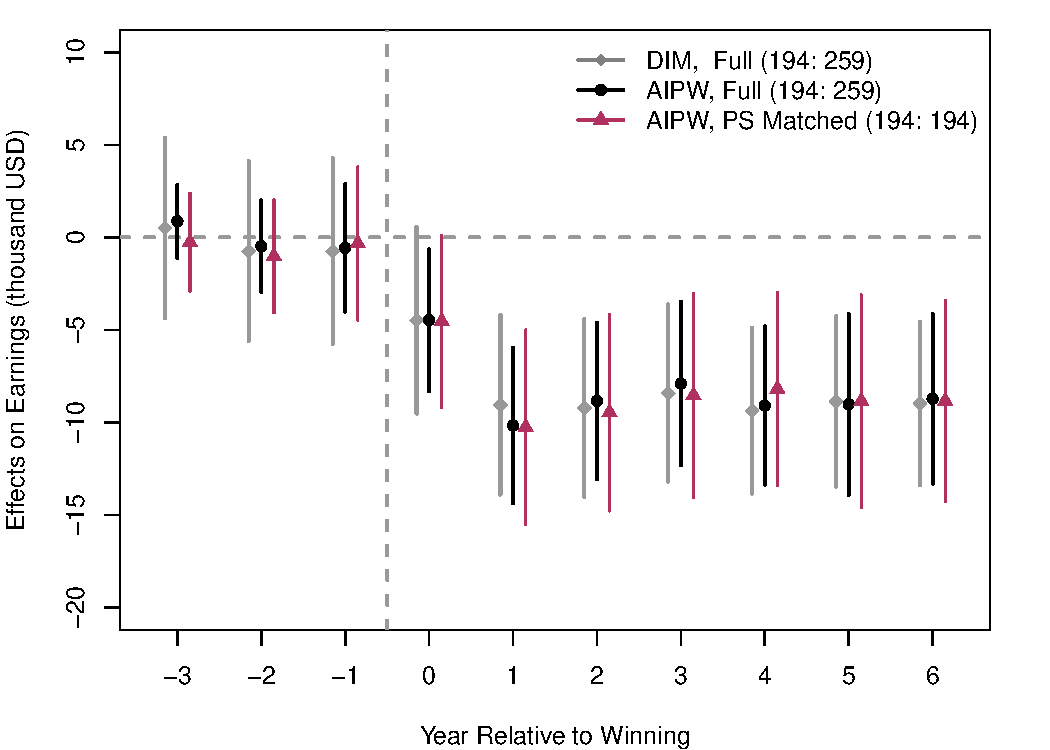
\includegraphics[width=1\linewidth]{irs1_dyn2.pdf}
            \caption{ATT: Big Winners vs Non-Winners}
        \end{subfigure}\hspace{1em}
        \begin{subfigure}{0.45\linewidth}
            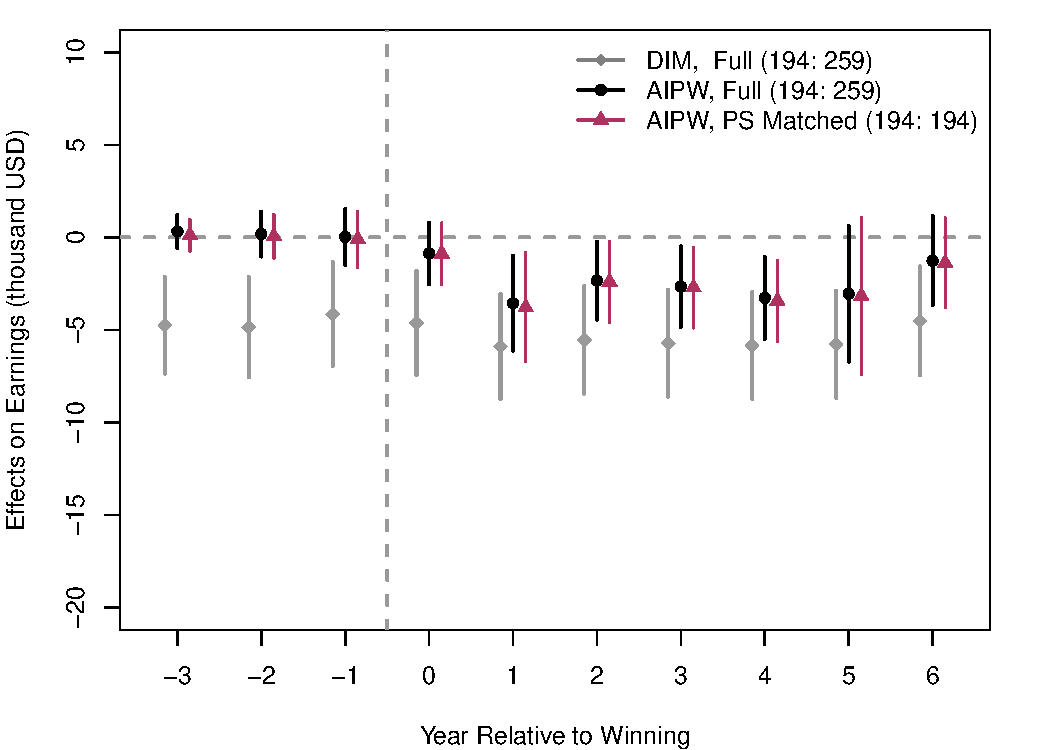
\includegraphics[width=1\linewidth]{irs2_dyn2.pdf}
            \caption{ATT: Small Winners vs Non-Winners}
        \end{subfigure}\\
        \hspace{-2em}\begin{subfigure}{0.45\linewidth}
        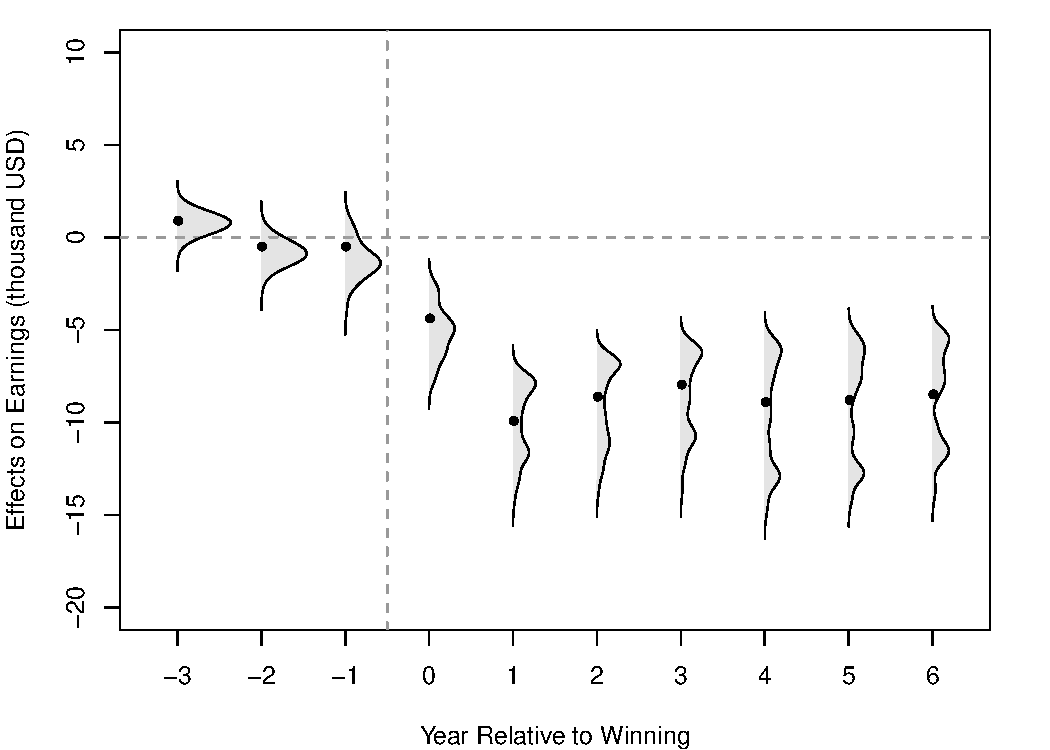
\includegraphics[width=\linewidth]{irs1_catt.pdf}
            \caption{CATT: Big Winners vs Non-Winners}
        \end{subfigure}\hspace{1em}
        \begin{subfigure}{0.45\linewidth}
            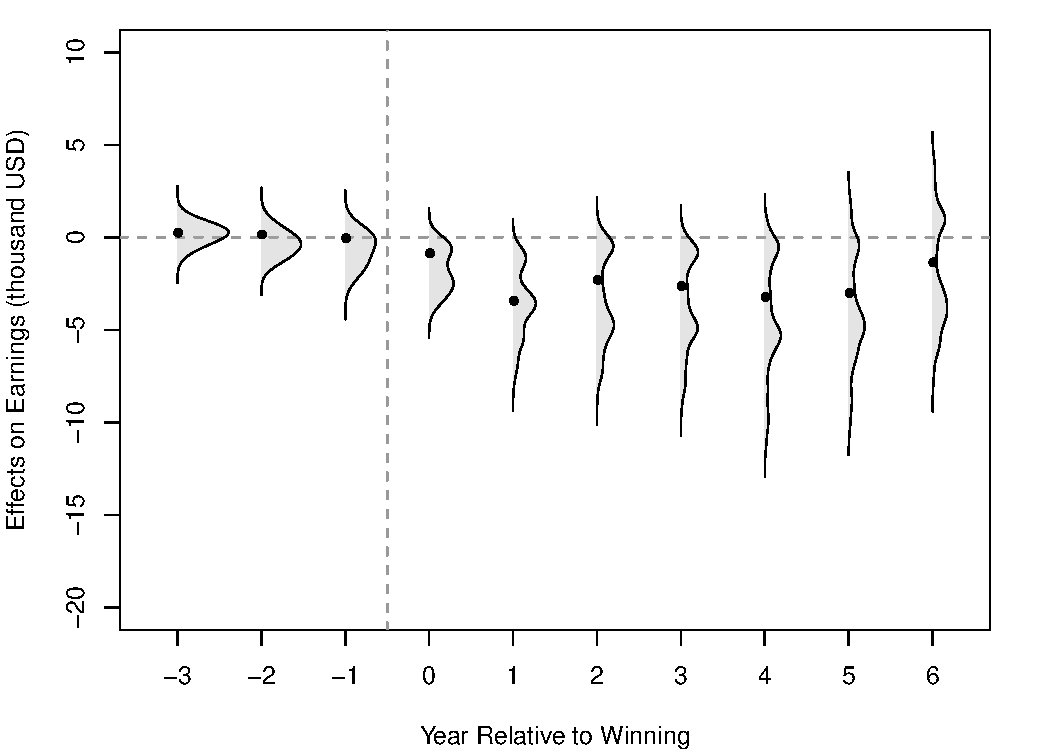
\includegraphics[width=\linewidth]{irs2_catt.pdf}
            \caption{CATT: Small Winners vs Non-Winners}
        \end{subfigure}
    \end{minipage}\\
    \raggedright
     {\footnotesize\textbf{\textit{Note:}} Figures show the ATT and CATT estimates using the IRS data. The outcome variables include earnings from 3 years before winning to 6 years after winning.  The estimates for pre-winning outcomes serve as placebo tests. Adjusted covariates include: time of playing, \#tickets bought, gender, work then, age at winning, years of education, college degree, and earnings 6 to 4 years before winning. \textbf{Subfigures A-B}: we use the difference-in-means estimator (gray diamonds) and the AIPW-GRF estimator (black solid circles for the original data and red triangles for the trimmed data).   \textbf{Subfigures C-D}: the distributions of CATT estimates using AIPW-GRF based on the full sample (with the black dots representing the corresponding ATT estimates).}
\end{figure}


We then estimate the ATT and CATT for labor income from Year $-3$ to Year $6$ separately using both difference-in-means and AIPW-GRF. The results are shown in Figure~\ref{fig:irs.est} (A) and (B). These representations closely resemble an event study plot used in panel data analysis although our main identification assumption is unconfoundedness. They show that in estimating the effect of big prizes, AIPW-GRF using the original or trimmed data produces estimates very similar to a simple difference-in-means estimator, suggesting minimal selection between the two groups. On the other hand, when estimating the effect of small prizes, the estimates from AIPW-GRF and difference-in-means diverge. However, findings from the former are much more credible than those from the latter because difference-in-means does not fare well in the placebo tests, whereas the former yields placebo estimates that are nearly zero. Figure~\ref{fig:irs.est}(C) and (D) display the CATT estimates (calculated at the covariate values of the treated units) for each of the ten outcomes in both comparisons. Beyond providing corroborative evidence for the placebo tests (i.e., CATT estimates align closely with 0 in the years leading up to the win), they also reveal substantial treatment effect heterogeneity among lottery winners. Notably, the distributions of the CATT for many post-winning years appear bimodal.

Overall, we find that in the lottery study, placebo tests provide strong evidence for the unconfoundedness assumption, bolstering the credibility of the causal estimates. Importantly, unconfoundedness is much more believable in this study than in the LaLonde case because the inherent randomization of lotteries played a key role in treatment assignment, while supplementary covariates help account for discrepancies between treatment and control groups stemming from challenges like differential responses to the survey. The inclusion of six preceding outcomes also proves invaluable, as they likely explain both selection and the outcome variables; moreover, they also serve as good candidates for placebo outcomes, given their comparability to these outcomes.


\section{Conclusion}\label{conclusion}

In his influential 1986 paper, Robert LaLonde critically evaluated nonexperimental methods, such as those based on linear regression methods and two-step selection models, by comparing their estimates to experimental benchmarks. He discovered that nonexperimental approaches produce highly variable estimates and fail to match experimental findings. Since then, there has been considerable progress in nonexperimental evaluation methodology. To illustrate these advances, we revisit the LaLonde and IRS datasets. Our analysis demonstrates that modern methods are effective in estimating adjusted group differences. A key caveat is that this relies on sufficient overlap. The estimates are less sensitive to the choice of the specific estimator. However, these estimates should be cautiously interpreted regarding causality, especially when there is a limited understanding of the assignment mechanism. In such cases, substantiating unconfoundedness is challenging and often requires supplementary analyses such as placebo tests. We show that unconfoundedness \emph{cannot} be credibly validated using the LaLonde nonexperimental data. In contrast, the IRS data, with its clear lottery-based assignment and extensive pretreatment information, makes unconfoundedness a more credible assumption.

Based on the lessons learned since \citet{LaLonde} in nearly four decades, we offer the following recommendations to practitioners: 
\begin{itemize}\itemsep0em
    \item Begin analyses of causal effects with an effort to understand the assignment mechanism. A clear grasp of the ``design'' is crucial for the credibility of the unconfoundedness assumption.
    \item Estimate the propensity score using a flexible method. Assess overlap by plotting the distributions of propensity scores for treated and control units. Trim the data based on the propensity score to make the groups more comparable. 
    \item Apply modern methods, such as doubly-robust estimators, to estimate the average causal effects. Explore alternative estimands, such as the conditional average treatment effects and quantile treatment effects. 
    \item Perform placebo tests, such as those using pretreatment outcomes, to validate unconfoundedness. Conduct sensitivity analyses to gauge the robustness of the findings. 
\end{itemize}
We provide an online tutorial with \texttt{R} code to assist researchers in implementing these methods.


\vspace{3em}
\clearpage
\bibliography{\bib}

\clearpage
\appendix
\onehalfspacing
\setcounter{page}{1}
\setcounter{table}{0}
\setcounter{figure}{0}
\setcounter{equation}{0}
\setcounter{footnote}{0}
\renewcommand\thetable{A\arabic{table}}
\renewcommand\thefigure{A\arabic{figure}}
\renewcommand{\thepage}{A-\arabic{page}}
\renewcommand{\theequation}{A\arabic{equation}}
\renewcommand{\thefootnote}{A\arabic{footnote}}

\vspace{0em}
\section{Tables 4-6 in LaLonde (1986)}
\bigskip

The following tables are adapted from Tables 4, 5, and 6 in \citet{LaLonde}. We thank Robert LaLonde's estate for allowing us to include these tables in the Appendix.

\begin{table}[!ht]
\includegraphics[scale = 0.4]{LaLonde_table4.png}
\end{table}
\clearpage

\begin{table}[!ht]
\includegraphics[scale = 0.4]{LaLonde_table5.png}
\end{table}
\clearpage


\begin{table}[!ht]
\includegraphics[scale = 0.4]{LaLonde_table6.png}
\end{table}

% bland page
\afterpage{\blankpage}
\clearpage


\onehalfspacing
\setcounter{page}{1}
\setcounter{table}{0}
\setcounter{figure}{0}
\setcounter{equation}{0}
\setcounter{footnote}{0}
\renewcommand\thetable{B\arabic{table}}
\renewcommand\thefigure{B\arabic{figure}}
\renewcommand{\thepage}{B-\arabic{page}}
\renewcommand{\theequation}{B\arabic{equation}}
\renewcommand{\thefootnote}{B\arabic{footnote}}

\vspace{0em}
\section{Online Supplementary Materials}
\bigskip


\noindent\hspace{-0.5em}{\bf \underline{Table of Contents}}

{\small
\begin{enumerate}\itemsep0.5em
    \item[B.1.] Additional Results Using the LDW Data
    \vspace{-0.5em}
    \begin{itemize}
        \item Assessing overlap
        \item ATT and placebo estimates
        \item CATT plots for placebo tests
        \item Sensitivity analyses
        \item ATT estimates without using '74 information
        \item CATT plots without using '74 information
    \end{itemize}
    \item[B.2.] Results based on the LaLonde Male Samples
    \vspace{-0.5em}
    \begin{itemize}
        \item Assessing overlap
        \item ATT estimates
        \item CATT estimates
        \item Quantile treatment effects
    \end{itemize}
    \item[B.2.] Results based on the Reconstructed Female Samples
    \vspace{-0.5em}
    \begin{itemize}
        \item Descriptive statistics
        \item Assessing overlap
        \item ATT estimates
        \item CATT estimates
        \item Quantile treatment effects
        \item Placebo test
    \end{itemize}
    \item[B.4.] Additional Results Using the IRS Data
    \vspace{-0.5em}
    \begin{itemize}
        \item Assessing overlap on the trimmed samples
        \item ATT and placebo estimates
        \item Results using the trimmed samples
        \item Quantile treatment effects
        \item Sensitivity analyses
    \end{itemize}    
\end{enumerate}
}

\clearpage



%%%%%%%%%%%%%%%%%%%%%%%%%%%%%

\subsection{Additional Results Using the LDW Data}

\paragraph{Assessing overlap} Figure~\ref{fig:overlap.ps} demonstrates overlap in the LDW data using the propensity scores estimated via GRF (instead of log odds). 


\begin{figure}[!ht]
    \caption{Assessing Overlaps in LDW Data: Propensity Scores}\label{fig:overlap.ps}
    \centering
    % First column
    \begin{minipage}[c]{.3\textwidth}
        \centering
        \begin{subfigure}{\linewidth} 
            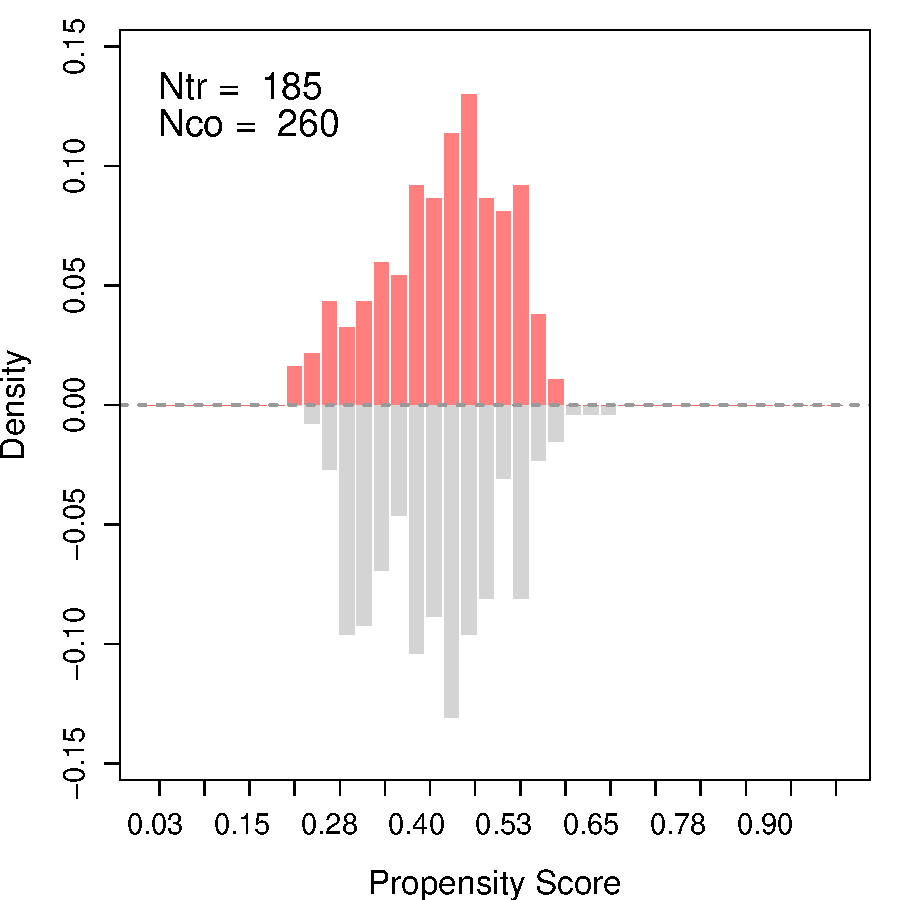
\includegraphics[width=\linewidth]{ps_ldw_exp.pdf}
            \caption{LDW-Experimental}
        \end{subfigure}
    \end{minipage}%
    % Second column
    \begin{minipage}[c]{.65\textwidth}
        \centering
        \begin{subfigure}{0.45\linewidth}
            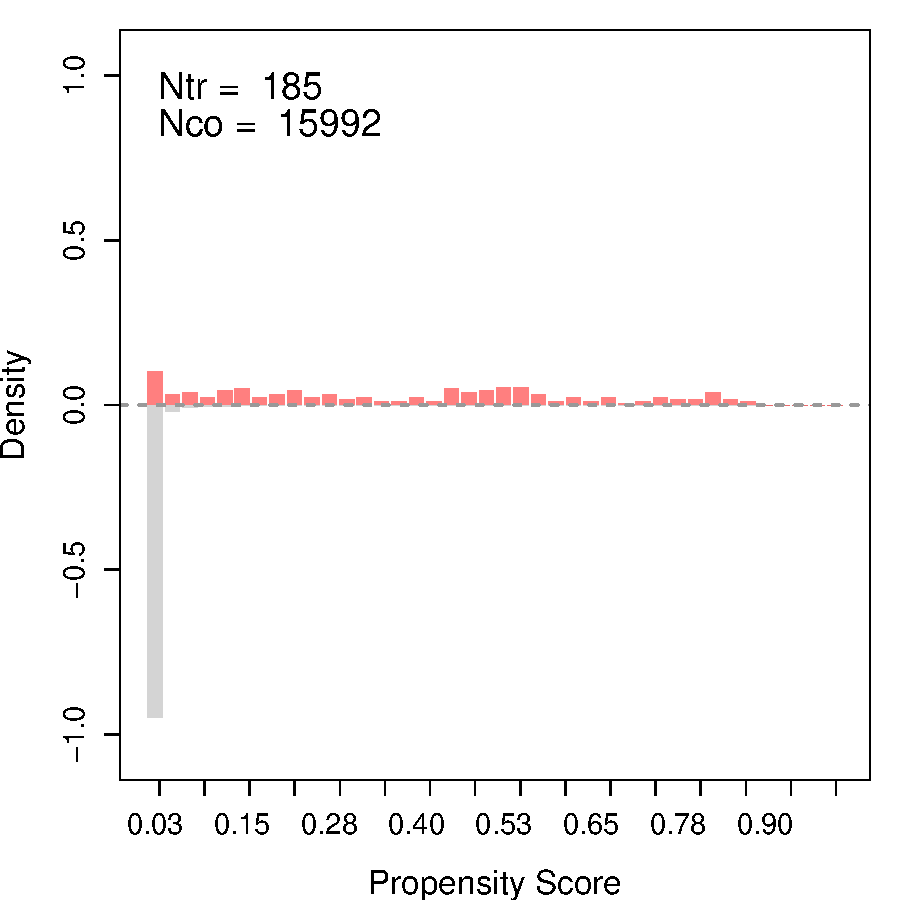
\includegraphics[width=\linewidth]{ps_ldw_cps.pdf}
            \caption{LDW-CPS}
        \end{subfigure}
        \begin{subfigure}{0.45\linewidth}
            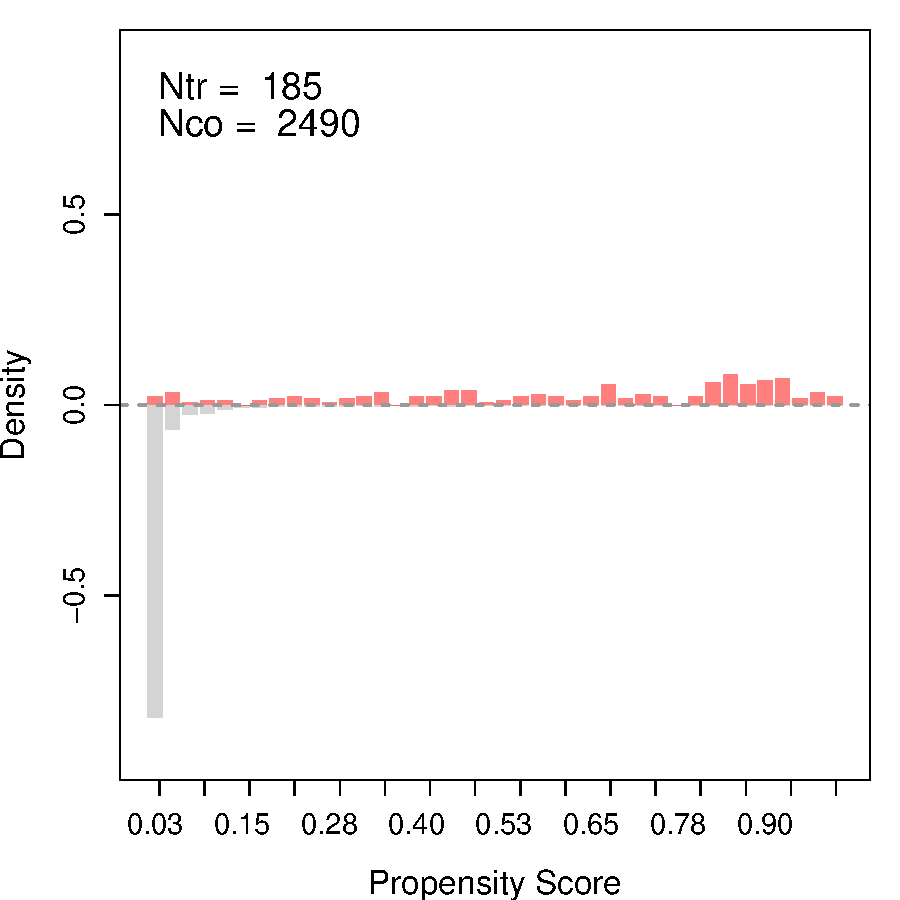
\includegraphics[width=\linewidth]{ps_ldw_psid.pdf}
            \caption{LDW-PSID}
        \end{subfigure}\\
        \begin{subfigure}{0.45\linewidth}
            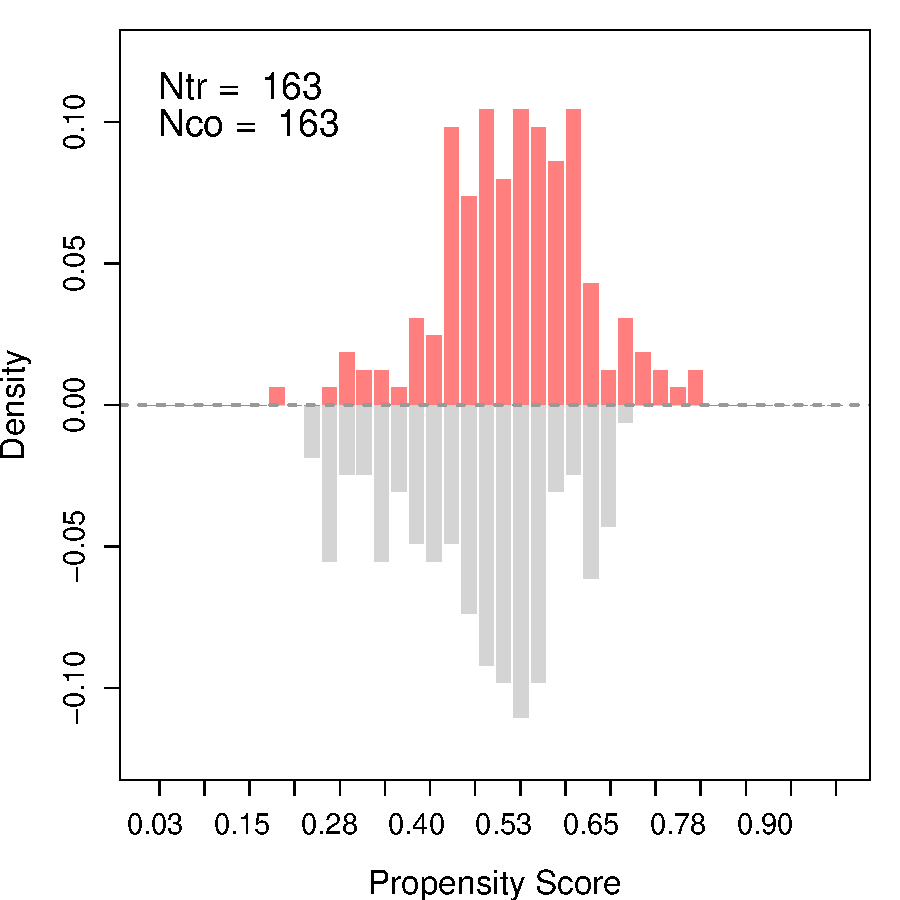
\includegraphics[width=\linewidth]{ps_ldw_cps_trim.pdf}
            \caption{LDW-CPS Trimmed}
        \end{subfigure}
        \begin{subfigure}{0.45\linewidth}
            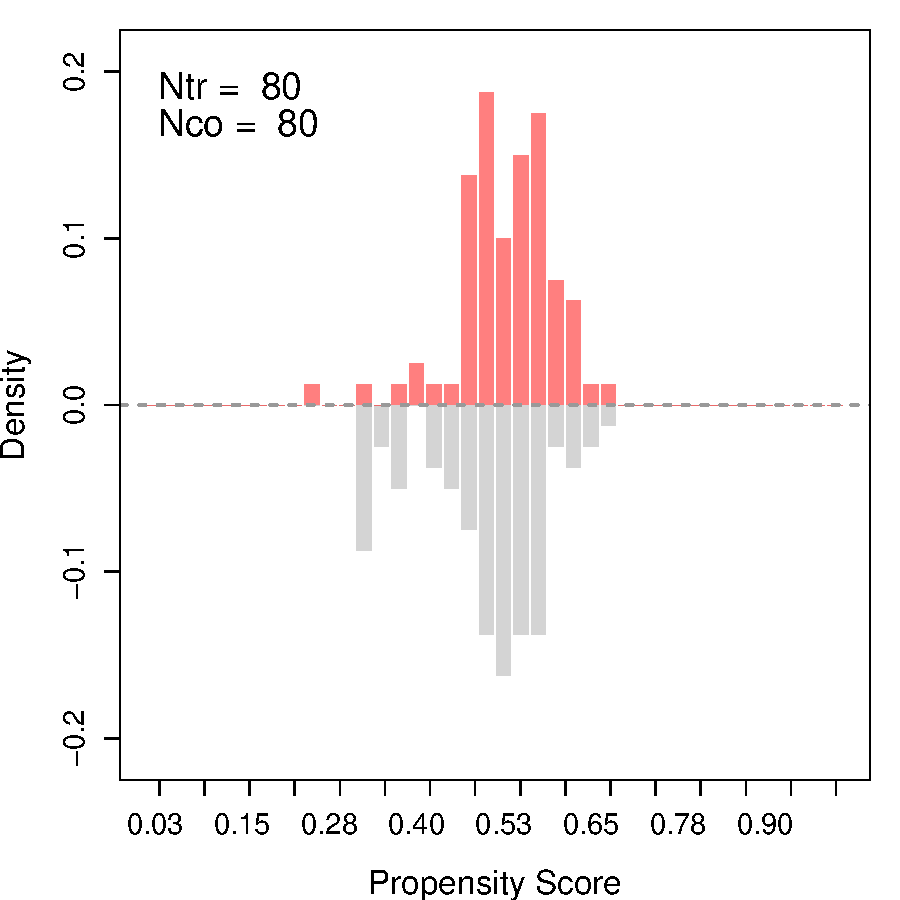
\includegraphics[width=\linewidth]{ps_ldw_psid_trim.pdf}
            \caption{LDW-PSID Trimmed}
        \end{subfigure}
    \end{minipage}%
    \\\raggedright
     {\footnotesize\textbf{\textit{Note:}} Histograms of the propensity scores estimated through GRF are depicted. Each subfigure represents a different sample. \textbf{Subfigure A}: LDW-Experimental. \textbf{Subfigure B}: LDW-CPS. \textbf{Subfigure C}: LDW-PSID. \textbf{Subfigure D}: Trimmed LDW-CPS. \textbf{Subfigure E}: Trimmed LDW-PSID. For C and D, the propensity scores are reestimated after trimming.}
\end{figure}
\FloatBarrier
\clearpage

\paragraph{ATT and placebo estimates} Table~\ref{tb:ldw.est} shows the ATT estimates using four different samples: LDW-CPS, LDW-PSID, trimmed LDW-CPS, and trimmed LDW-PSID. The ATT estimates based on the experimental benchmarks are highlighted in bold font in the first row. These estimates are visualized in Figure~\ref{fig:ldw.att} in the main text.

\begin{table}[!ht]
\caption{ATT Estimates under Unconfoundedness: LDW Samples}\label{tb:ldw.est}
\begin{minipage}[c]{1\textwidth}
\vspace{-0.5em}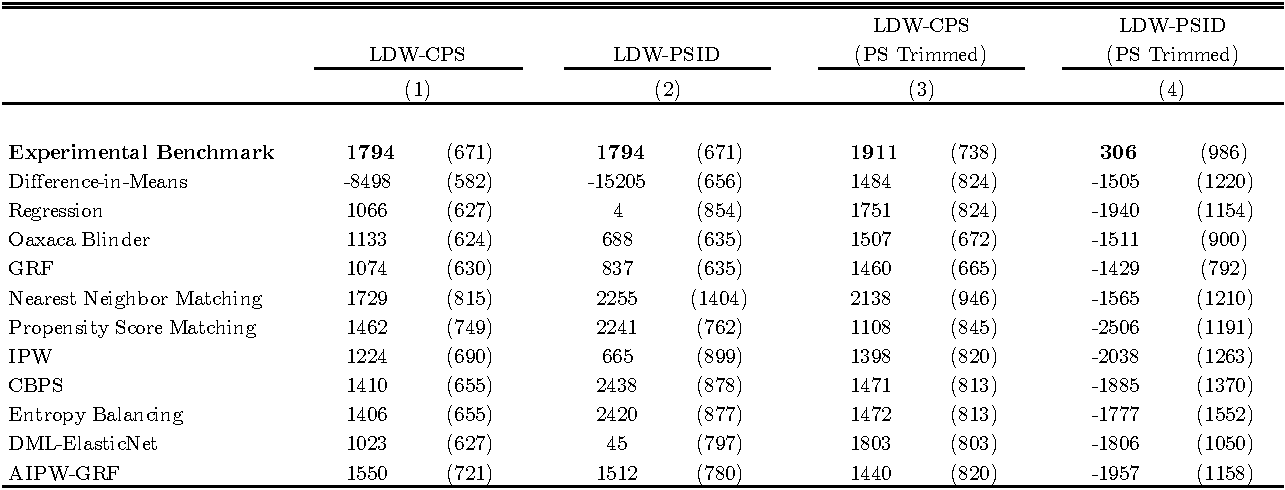
\includegraphics[width=\linewidth]{ldw.pdf}
{\footnotesize\textbf{\textit{Note:}} ATT estimates using the LDW data. The outcome variable is \texttt{re78}. We adjust for the following covariates: \texttt{age}, \texttt{education}, \texttt{black}, \texttt{hispanic}, \texttt{married}, \texttt{nodegree}, \texttt{re74}, \texttt{u74}, \texttt{re75}, and \texttt{u75}. The trimmed samples are based on 1:1 matching on propensity scores estimated via GRF. Robust standard errors are in the parentheses.}
\end{minipage}%
\end{table}

\clearpage

Table~\ref{tb:ldw.placebo} shows the results of the placebo analyses using earnings in 1975 (\texttt{re75}) as the placebo outcome and remove both \texttt{re75} and \texttt{u75} from the set of conditioning variables. These estimates are visualized in Figure~\ref{fig:ldw.placebo} in the main text.

\begin{table}[!ht]
\caption{Placebo Test: '75 Earnings as the Outcome}\label{tb:ldw.placebo}
\begin{minipage}[c]{1\textwidth}
\vspace{-0.5em}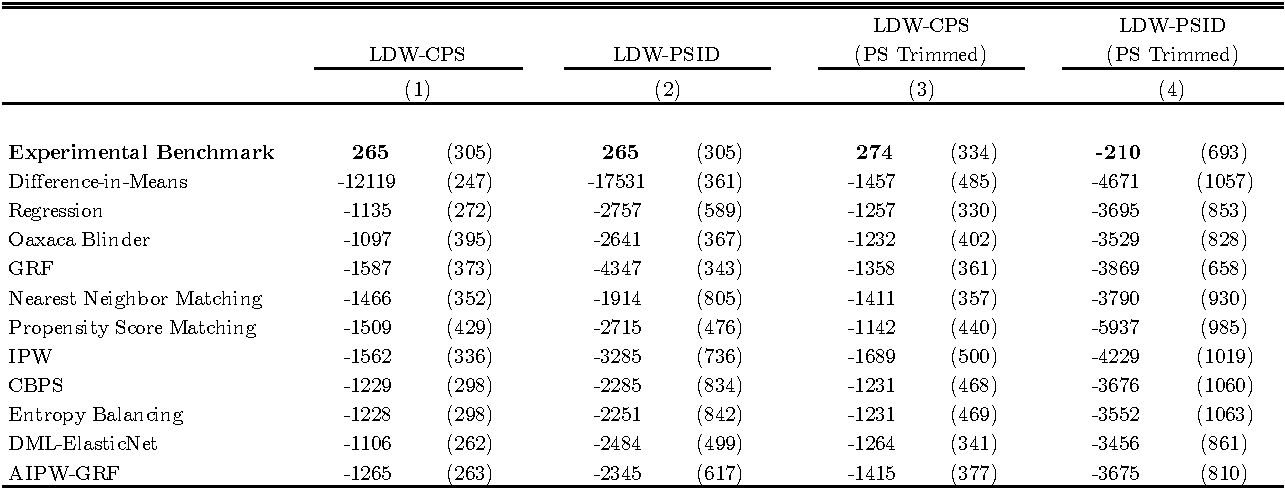
\includegraphics[width=\linewidth]{ldw_placebo.pdf}
{\footnotesize\textbf{\textit{Note:}} ATT estimates using the LDW data. The outcome variable is \texttt{re75}. We adjust for the following covariates: \texttt{age}, \texttt{education}, \texttt{black}, \texttt{hispanic}, \texttt{married}, \texttt{nodegree}, \texttt{re74}, and \texttt{u74}.  The trimmed samples are based on 1:1 matching on propensity score estimated via GRF. Robust standard errors are in the parentheses.}
\end{minipage}%
\end{table}

\clearpage

\paragraph{CATT plots for placebo tests} Figure~\ref{fig:ldw.catt.placebo} shows that the CATT estimates using 1975 earnings as the placebo outcome. 

\begin{figure}[!ht]
    \caption{Placebo Tests using LDW Data: Experimental vs. Nonexperimental}\label{fig:ldw.catt.placebo}
    \vspace{-1em}
    \begin{minipage}[c]{1\textwidth}
        \centering
        \begin{subfigure}{0.4\linewidth}
            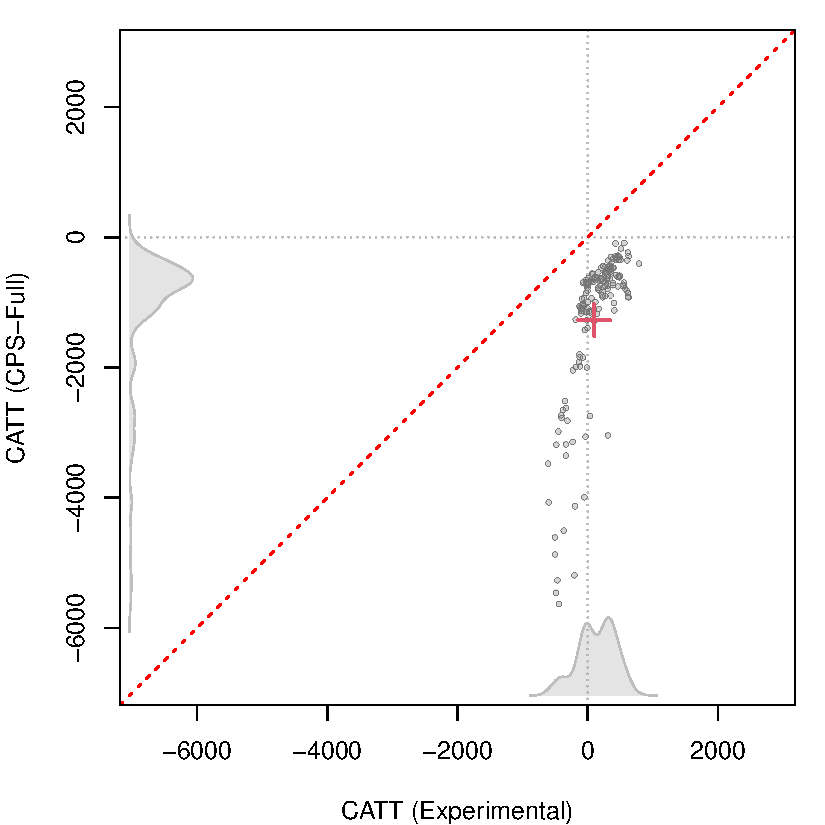
\includegraphics[width=\linewidth]{catt_placebo_cps.pdf}
            \caption{LDW-CPS}
        \end{subfigure}
        \begin{subfigure}{0.4\linewidth}
            \includegraphics[width=\linewidth]{catt_placebo_PSID.pdf}
            \caption{LDW-PSID}
        \end{subfigure}\\
        \begin{subfigure}{0.4\linewidth}
            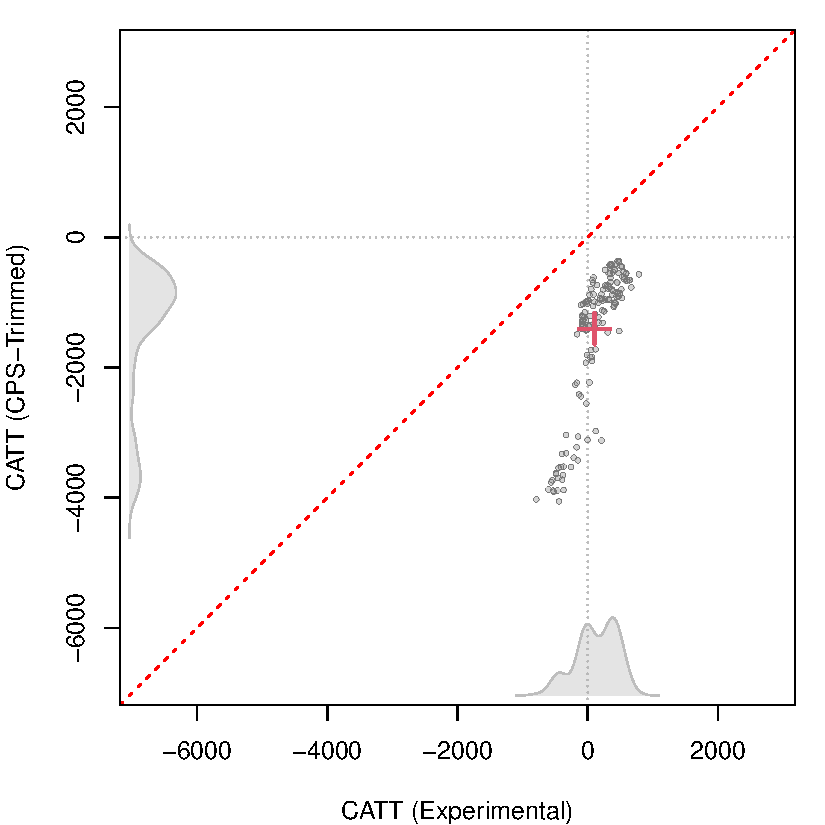
\includegraphics[width=\linewidth]{catt_placebo_cps_trim.pdf}
            \caption{LDW-CPS Trimmed}
        \end{subfigure}
        \begin{subfigure}{0.4\linewidth}
            \includegraphics[width=\linewidth]{catt_placebo_PSID_trim.pdf}
            \caption{LDW-PSID Trimmed}
        \end{subfigure}
    \end{minipage}%
    \\\raggedright
     {\footnotesize\textbf{\textit{Note:}} Scatterplots show the CATT on a placebo outcome, real earning in 1975 (\texttt{re75}), using both experimental data (x-axis) and nonexperimental data (y-axis). Each dot corresponds to a CATT estimate based on the covariate values of a treated unit, while each red cross symbolizes the ATT estimates. For every estimate, the AIPW estimator is employed, with the GRF approach for estimating nuisance parameters. Different subfigures indicate various data comparisons: \textbf{Subfigure A}: Compares LDW-Experimental with LDW-CPS. \textbf{Subfigure B}: Compares LDW-Experimental with LDW-PSID. \textbf{Subfigure C}: Compares trimmed LDW-Experimental (removing 22 treated units) against trimmed LDW-CPS. \textbf{Subfigure D}: Compares trimmed LDW-Experimental (removing 70 treated units) to trimmed LDW-PSID.}
\end{figure}
\clearpage


\paragraph{Sensitivity analyses} Figure~\ref{fig:ldw.sens} shows the results of the sensitivity analyses using the trimmed LDW data, including trimmed LDW-CPS and trimmed LDW-PSID. We used 1975 earnings (\texttt{re75}) as the benchmark covariate. The analysis suggests that the estimated training effect based on LDW-CPS is less sensitive to potential confounders compared to trimmed LDW-PSID. 

\begin{figure}[!ht]
    \caption{Sensitivity Analyses for Trimmed LDW-CPS and LDW-PSID}\label{fig:ldw.sens}
    \begin{minipage}[c]{1\textwidth}
        \centering
        \begin{subfigure}{0.45\linewidth}
            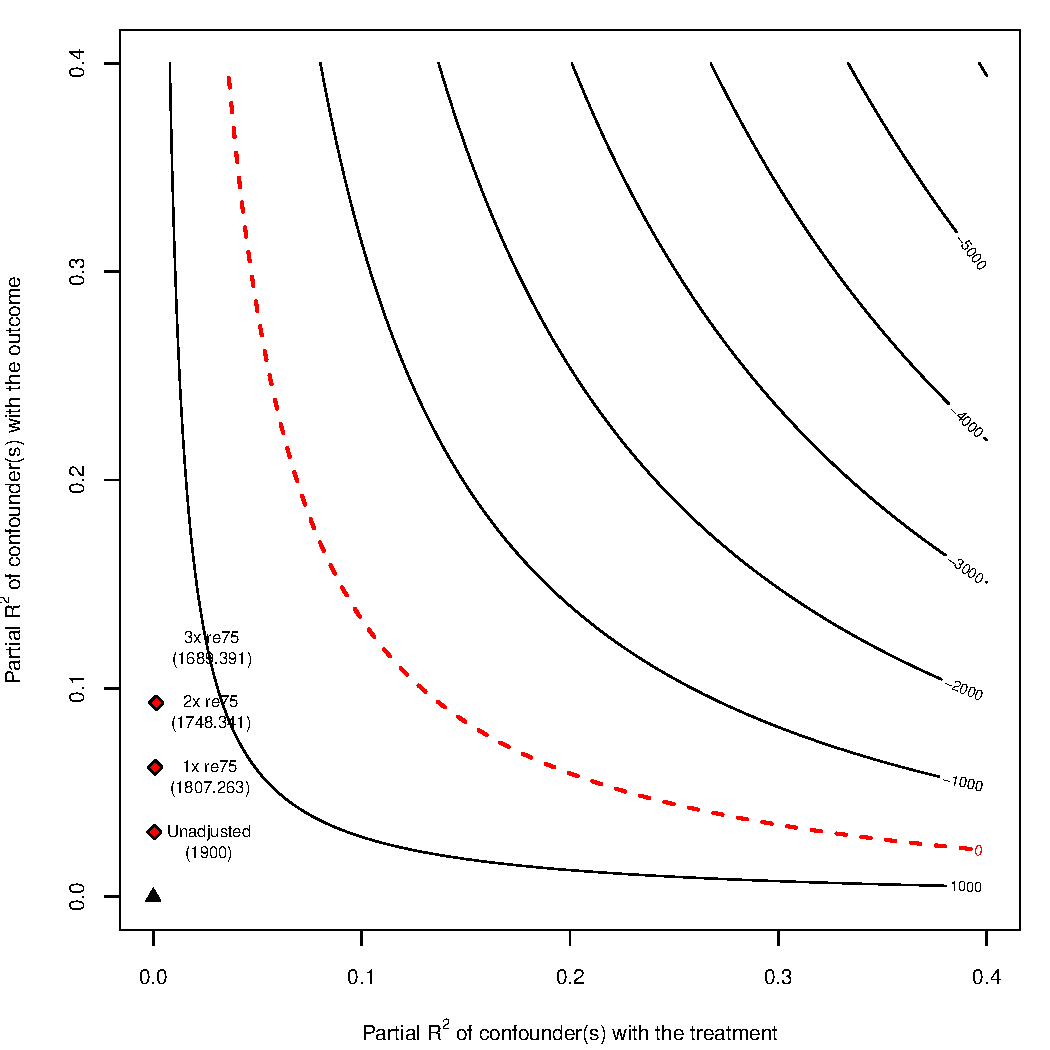
\includegraphics[width=\linewidth]{sens_ldw_cps.pdf}
            \caption{LDW-CPS}
        \end{subfigure}\hspace{1em}
        \begin{subfigure}{0.45\linewidth}
            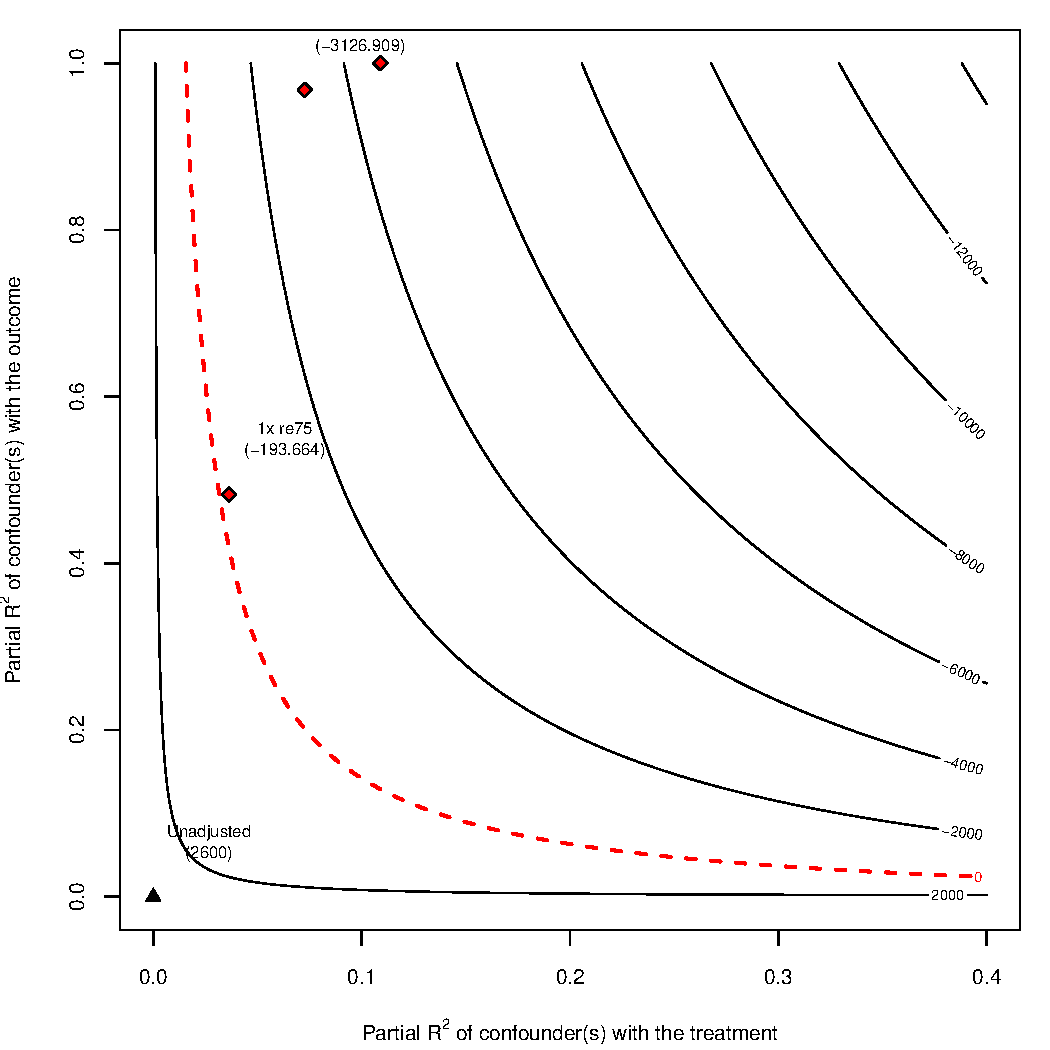
\includegraphics[width=\linewidth]{sens_ldw_psid.pdf}
            \caption{LDW-PSID}
        \end{subfigure}
    \end{minipage}%
    \\\raggedright
     {\footnotesize\textbf{\textit{Note:}} Contour plot for the treatment effect coefficient $\hat{\tau}_{OLS}$ based on sensitivity analysis first proposed by \citet{imbens2003} and then modified by \citet{cinelli2020making}. The red dashed line indicates $\hat\tau_{OLS} = 0$. The benchmark covariate is \texttt{re75}. The model is a linear regression with all available long-term covariates included. Both datasets are preprocessed by trimming observations whose estimated propensity scores are smaller than 0.1 or bigger than 0.9.}
\end{figure}
\clearpage


\paragraph{ATT Estimates without using '74 information}

Table~\ref{tb:ldw.no74.est} presents ATT estimates based on the LDW samples without using earnings  and employment status in 1974.

\begin{table}[!ht]
\caption{ATT Estimates without Using \texttt{re74} and \texttt{u74}: LDW Samples}\label{tb:ldw.no74.est}
\begin{minipage}[c]{1\textwidth}
\vspace{-0.5em}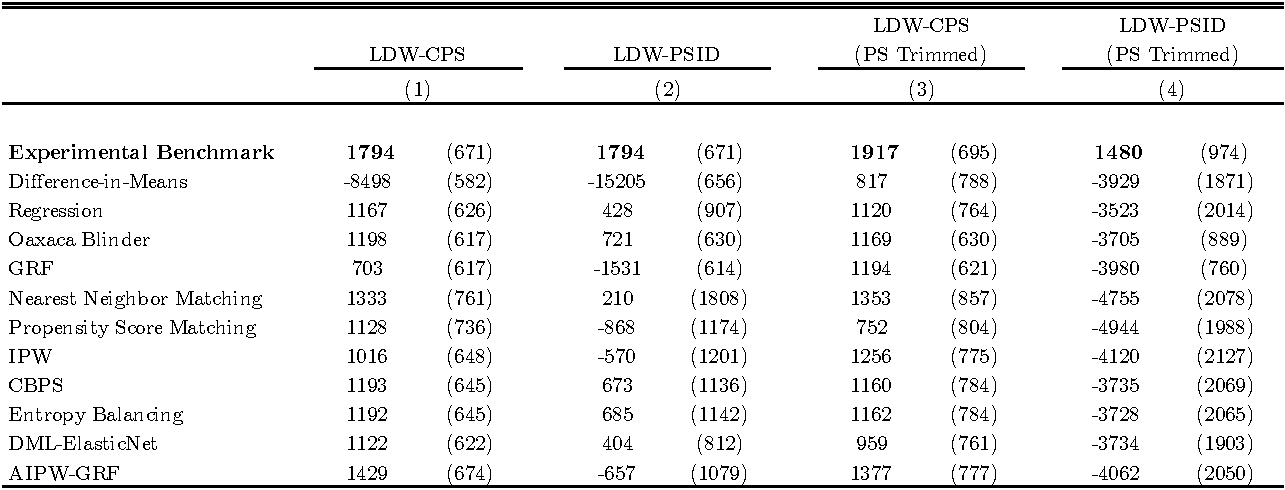
\includegraphics[width=\linewidth]{ldw_no74.pdf}
{\footnotesize\textbf{\textit{Note:}} ATT estimates using the LDW data. The outcome variable is \texttt{re78}. We adjust for the following covariates: \texttt{age}, \texttt{education}, \texttt{black}, \texttt{hispanic}, \texttt{married}, \texttt{nodegree}, \texttt{re75}, and \texttt{u75}. The trimmed samples are based on 1:1 matching on propensity scores estimated via GRF. Robust standard errors are in the parentheses.}
\end{minipage}%
\end{table}

\clearpage

\paragraph{CATT plots without using '74 information} Figure~\ref{fig:no74} shows that the CATT estimates without using 1974 earnings and employment status. 

\begin{figure}[!ht]
    \caption{Placebo Tests using LDW Data: Experimental vs. Nonexperimental}\label{fig:no74}
    \vspace{-1em}
    \begin{minipage}[c]{1\textwidth}
        \centering
        \begin{subfigure}{0.4\linewidth}
            \includegraphics[width=\linewidth]{catt_no74_cps.pdf}
            \caption{LDW-CPS}
        \end{subfigure}
        \begin{subfigure}{0.4\linewidth}
            \includegraphics[width=\linewidth]{catt_no74_PSID.pdf}
            \caption{LDW-PSID}
        \end{subfigure}\\
        \begin{subfigure}{0.4\linewidth}
            \includegraphics[width=\linewidth]{catt_no74_cps_trim.pdf}
            \caption{LDW-CPS Trimmed}
        \end{subfigure}
        \begin{subfigure}{0.4\linewidth}
            \includegraphics[width=\linewidth]{catt_no74_PSID_trim.pdf}
            \caption{LDW-PSID Trimmed}
        \end{subfigure}
    \end{minipage}%
    \\\raggedright
     {\footnotesize\textbf{\textit{Note:}} Scatterplots show the CATT on real earning in 1978 (\texttt{re78}), using both experimental data (x-axis) and nonexperimental data (y-axis), but without using 1974 earnings and employment status. . Each dot corresponds to a CATT estimate based on the covariate values of a treated unit, while each red cross symbolizes the ATT estimates. For every estimate, the AIPW estimator is employed, with the GRF approach for estimating nuisance parameters. Different subfigures indicate various data comparisons: \textbf{Subfigure A}: Compares LDW-Experimental with LDW-CPS. \textbf{Subfigure B}: Compares LDW-Experimental with LDW-PSID. \textbf{Subfigure C}: Compares trimmed LDW-Experimental (removing 10 treated units) against trimmed LDW-CPS. \textbf{Subfigure D}: Compares trimmed LDW-Experimental (removing 106 treated units) to trimmed LDW-PSID.}
\end{figure}
\clearpage


\FloatBarrier

\clearpage

\subsection{Results based on the LaLonde Male Samples}

Two pretreatment variables, earnings in 1974 and employment status in 1974 are absent from this sample.

\paragraph{Assessing overlap} Figure~\ref{fig:nsw.overlap} demonstrates overlap in the LDW using the propensity score estimated via GRF (log odds ratio). 


\begin{figure}[!ht]
    \caption{Assessing the Overlap in the LaLonde Data (Male Sample)}\label{fig:nsw.overlap}
    \centering
    % First column
    \begin{minipage}[c]{.3\textwidth}
        \centering
        \begin{subfigure}{\linewidth}
            \includegraphics[width=\linewidth]{odds_nsw_exp.pdf}
            \caption{LDW-Experimental}
        \end{subfigure}
    \end{minipage}%
    % Second column
    \begin{minipage}[c]{.65\textwidth}
        \centering
        \begin{subfigure}{0.45\linewidth}
            \includegraphics[width=\linewidth]{odds_nsw_cps.pdf}
            \caption{LaLonde-CPS1}
        \end{subfigure}
        \begin{subfigure}{0.45\linewidth}
            \includegraphics[width=\linewidth]{odds_nsw_psid.pdf}
            \caption{LaLonde-PSID1}
        \end{subfigure}\\
        \begin{subfigure}{0.45\linewidth}
            \includegraphics[width=\linewidth]{odds_nsw_cps_trim.pdf}
            \caption{Trimmed LaLonde-CPS1}
        \end{subfigure}
        \begin{subfigure}{0.45\linewidth}
            \includegraphics[width=\linewidth]{odds_nsw_psid_trim.pdf}
            \caption{Trimmed LaLonde-PSID1}
        \end{subfigure}
    \end{minipage}%
    \\\raggedright
     {\footnotesize\textbf{\textit{Note:}} Histograms depict the log odds ratios, i.e., $\log\frac{\hat{e}}{1-\hat{e}}$, using propensity score estimated through GRF. Each subfigure represents a different sample. \textbf{Subfigure A}: Experimental (male sample). \textbf{Subfigure B}: LaLonde-CPS1. \textbf{Subfigure C}: LaLonde-PSID1. \textbf{Subfigure D}: Trimmed LaLonde-CPS1. \textbf{Subfigure E}: Trimmed LaLonde-PSID1. For C and D, the propensity scores are reestimated after trimming. Covariates do not include \texttt{re74} and \texttt{u74}.}
\end{figure}
\clearpage

\paragraph{ATT estimates} Table~\ref{tb:nsw.est} shows the ATT estimates using the original LaLonde male samples, of which the LDW sample is a subset. Two covariates, \texttt{re74} and \texttt{u74}, are absent from this sample. CPS-SSA-1 and PSID-1 are used as nonexperimental control groups. We also trim the data to improve overlap, using the same procedure applied to the LDW samples. Figure~\ref{fig:nsw.est} visualizes the ATT estimates.

\begin{table}[!ht]
\caption{ATT Estimates: LaLonde Male Samples}\label{tb:nsw.est}
\begin{minipage}[c]{1\textwidth}
\vspace{-0.5em}\includegraphics[width=\linewidth]{nsw.pdf}
{\footnotesize\textbf{\textit{Note:}} ATT estimates using the orignal LaLonde data (male sample). The control groups are CPS-SSA-1 (CPS1) and PSID-1 (PSID1). The outcome variable is \texttt{re78}. We adjust for the following covariates: \texttt{age}, \texttt{education}, \texttt{black}, \texttt{hispanic}, \texttt{married}, \texttt{nodegree}, \texttt{re75}, and \texttt{u75}. The trimmed samples are based on 1:1 matching on propensity score estimated via GRF. Robust standard errors are in the parentheses.}
\end{minipage}%
\end{table}

\clearpage

\begin{figure}[!ht]
    \caption{ATT Estimates Given Unconfoundedness: LaLonde Male Samples}\label{fig:nsw.att}
    \vspace{-1em}
    \begin{minipage}[c]{1\textwidth}
    \begin{center}
    \includegraphics[width=0.8\linewidth]{coef_nsw_cps.pdf}
    \includegraphics[width=0.8\linewidth]{coef_nsw_psid.pdf}
    \includegraphics[width=0.8\linewidth]{coef_nsw_cps_trim.pdf}
    \includegraphics[width=0.8\linewidth]{coef_nsw_psid_trim.pdf}
    \end{center}    
     {\footnotesize\textbf{\textit{Note:}} The above figures show the ATT estimates and their 95\% confidence intervals using four different samples: NSW-CPS, NSW-PSID, Trimmed NSW-CPS, and Trimmed NSW-PSID. Eleven estimators are employed, including difference-in-means, linear regression, Oaxaca Blinder, GRF as an outcome model, 1: 5 nearest neighbor matching with bias correction, propensity score matching, IPW with propensity scores estimated by GRF, CBPS, entropy balancing, double/debiased matching learning with elastic net (implemented using \texttt{DoubleML}), and AIPW with GRF  (implemented using \texttt{grf}). The red dashed line and pink band represent the experiment benchmark and its 95\% confidence intervals, respectively.}
     \end{minipage}
\end{figure}


\clearpage


\paragraph{CATT estimates}  Figure~\ref{fig:nsw.catt} shows the CATT estimates using the original LaLonde data (male sample). Two covariates, \texttt{re74} and \texttt{u74}, are not included in this sample.

\begin{figure}[!ht]
    \caption{CATT Estimates for the LaLonde Data (Male Sample)}\label{fig:nsw.catt}
    \centering
    \begin{minipage}[c]{1\textwidth}
        \centering
        \begin{subfigure}{0.4\linewidth}
            \includegraphics[width=\linewidth]{catt_nsw_cps.pdf}
            \caption{NSW-CPS}
        \end{subfigure}
        \begin{subfigure}{0.4\linewidth}
            \includegraphics[width=\linewidth]{catt_nsw_psid.pdf}
            \caption{NSW-PSID}
        \end{subfigure}\\
        \begin{subfigure}{0.4\linewidth}
            \includegraphics[width=\linewidth]{catt_nsw_cps_trim.pdf}
            \caption{NSW-CPS Trimmed}
        \end{subfigure}
        \begin{subfigure}{0.4\linewidth}
            \includegraphics[width=\linewidth]{catt_nsw_psid_trim.pdf}
            \caption{NSW-PSID Trimmed}
        \end{subfigure}
    \end{minipage}%
    \\\raggedright
     {\footnotesize\textbf{\textit{Note:}} Scatterplots show the CATT using both experimental data (x-axis) and nonexperimental data (y-axis) from \citet{LaLonde} (male sample). Each dot corresponds to a CATT estimate based on the covariate values of a treated unit, while each red cross symbolizes the ATT estimates. For every estimate, the AIPW estimator is employed, with the GRF approach for estimating nuisance parameters. Different subfigures indicate various data comparisons: \textbf{Subfigure A}: Compares Experimental with LaLonde-CPS1. \textbf{Subfigure B}: Compares Experimental with LaLonde-PSID1. \textbf{Subfigure C}: Compares trimmed Experimental (removing 30 treated units) against trimmed NSW-CPS. \textbf{Subfigure D}: Compares trimmed Experimental (removing 150 treated units) to trimmed NSW-PSID.}
\end{figure}
\clearpage

\paragraph{Quantile treatment effects} Figures~\ref{fig:nsw.qte} shows the quantile treatment effects on the treated using the original LaLonde (NSW) male samples. 

\begin{figure}[!ht]
    \caption{Quantile Treatment Effects: Experimental vs. Nonexperimental}\label{fig:nsw.qte}
    \begin{minipage}[c]{1\textwidth}
        \centering\vspace{-1em}
        \begin{subfigure}{1\linewidth}\hspace{1em}\centering
            \includegraphics[width=0.45\linewidth]{qte_nsw_cps.pdf}\hspace{2em}
            \includegraphics[width=0.45\linewidth]{qte_nsw_cps_trim.pdf}
            \caption{NSW-CPS}
        \end{subfigure}\\
        \begin{subfigure}{1\linewidth}\hspace{1em}\centering
            \includegraphics[width=0.45\linewidth]{qte_nsw_psid.pdf}\hspace{2em}
            \includegraphics[width=0.45\linewidth]{qte_nsw_psid_trim.pdf}
            \caption{NSW-PSID}
        \end{subfigure}
    \end{minipage}%
    \\\raggedright
     {\footnotesize\textbf{\textit{Note:}} Figures show the quantile treatment effects on the treated (QTET) using both experimental data (in blue) and nonexperimental data (in red for raw estimates and black for covariate-adjusted estimates). Each dot corresponds to a QTET estimate at a particular quantile, while shaded areas represent bootstrapped 95\% confidence intervals. Unadjusted models do not incorporate covariates while adjustment models use the full set of covariates to estimate the propensity scores with a logit. \textbf{Subfigure A}: Compares NSW experimental data with NSW-CPS. \textbf{Subfigure B}: Compares NSW experimental data with NSW-PSID.}
\end{figure}
\clearpage


\paragraph{Sensitivity analyses} Figure~\ref{fig:nsw.sens} shows the results of the sensitivity analyses using the trimmed LaLonde male samples, including trimmed NSW-CPS and trimmed NSW-PSID. We used 1975 earnings (\texttt{re75}) as the benchmark covariate. The analysis suggests that the estimated training effects are robust to potential confounders that behavior like \texttt{re75}. For instance, with trimmed NSW-CPS or NSW-PSID, the estimate remains positive and substantial even when a confounder's correlations with treatment and outcome are triple those of \texttt{re75}.

\begin{figure}[!ht]
    \caption{Sensitivity Analyses for Trimmed NSW-CPS and NSW-PSID}\label{fig:nsw.sens}
    \begin{minipage}[c]{1\textwidth}
        \centering
        \begin{subfigure}{0.45\linewidth}
            \includegraphics[width=\linewidth]{sens_nsw_cps.pdf}
            \caption{LDW-CPS}
        \end{subfigure}\hspace{1em}
        \begin{subfigure}{0.45\linewidth}
            \includegraphics[width=\linewidth]{sens_nsw_psid.pdf}
            \caption{LDW-PSID}
        \end{subfigure}
    \end{minipage}%
    \\\raggedright
     {\footnotesize\textbf{\textit{Note:}} Contour plot for the treatment effect coefficient $\hat{\tau}_{OLS}$ based on sensitivity analysis first proposed by \citet{imbens2003} and then modified by \citet{cinelli2020making}. The red dashed line indicates $\hat\tau_{OLS} = 0$. The benchmark covariate is \texttt{re75}. The model is a linear regression with all available long-term covariates included. Both datasets are preprocessed by trimming observations whose estimated propensity scores are smaller than 0.1 or bigger than 0.9.}
\end{figure}
\clearpage


\subsection{Results based on the Reconstructed LaLonde Female Samples}

We report findings using the LaLonde female samples reconstructed by \citet{calonico2017women}, referred to as the LaLonde-Cal{\'o}nico-Smith (LCS) sample. Consistent with LaLonde's original analysis, the outcome variable is earnings in 1979 (\texttt{re79}). We use the same set of covariates as in \citet{LaLonde}. Notably, this set does not include two pretreatment variables: earnings in 1974 and employment status in 1974. We also exclude the number of children in 1975 (\texttt{nchildren75}), which is available in the LCS dataset, from the covariates so that it can serve as a placebo outcome. We also trim the data to improve overlap, using the same procedure applied to the LDW samples. The threshold for the propensity score to trim the sample in Step (A) is set at 0.9. 

\paragraph{Descriptive statistics} Table~\ref{tb:samples_lcs} shows the descriptive statistics of the reconstructed LaLonde female sample. 

\begin{table}[!ht]
\caption{Descriptive Statistics: LCS Female Samples}\label{tb:samples_lcs}
\begin{minipage}[c]{0.9\textwidth}
\vspace{-0.5em}\includegraphics[width=\linewidth]{stats_lcs.pdf}
{\footnotesize\textbf{\textit{Note:}} Standard deviations are in the parentheses.}
\end{minipage}%
\end{table}
\clearpage

\paragraph{Assessing overlap} Figure~\ref{fig:lcs.overlap} demonstrates overlap in the LDW using the propensity score estimated via GRF (log odds ratio). 


\begin{figure}[!ht]
    \caption{Assessing the Overlap in the Reconstructed LaLonde Female Samples}\label{fig:lcs.overlap}
    \centering
    \begin{minipage}[c]{\textwidth}
        \centering
        \begin{subfigure}{0.32\linewidth}
            \includegraphics[width=\linewidth]{odds_lcs_exp.pdf}
            \caption{LCS-Experimental}
        \end{subfigure}
        \begin{subfigure}{0.32\linewidth}
            \includegraphics[width=\linewidth]{odds_lcs_psid.pdf}
            \caption{LCS-PSID}
        \end{subfigure}
         \begin{subfigure}{0.32\linewidth}
            \includegraphics[width=\linewidth]{odds_lcs_psid_trim.pdf}
            \caption{Trimmed LCS-PSID}
        \end{subfigure}
    \end{minipage}%
    \\\raggedright
     {\footnotesize\textbf{\textit{Note:}} Histograms depict the log odds ratios, i.e., $\log\frac{\hat{e}}{1-\hat{e}}$, using propensity score estimated through GRF. Each subfigure represents a different sample. \textbf{Subfigure A}: LCS-Experimental. \textbf{Subfigure B}: LCS-PSID. \textbf{Subfigure C}: Trimmed LCS-PSID. For C, the propensity score is reestimated after trimming. Covariates do not include \texttt{re74}, \texttt{u74}, and \texttt{nchildren75}.}
\end{figure}
\clearpage

\paragraph{ATT estimates} Table~\ref{tb:lcs.est} shows the ATT estimates using the reconstructed LaLonde female samples. Reconstructed PSID-1 is used as the nonexperimental control group.  Figure~\ref{fig:lcs.att} visualizes the ATT estimates.

\begin{table}[!ht]
\caption{ATT Estimates: Reconstructed LaLonde Female Samples}\label{tb:lcs.est}
\begin{minipage}[c]{1\textwidth}
\begin{center}
\vspace{-0.5em}\includegraphics[width=0.6\linewidth]{lcs.pdf}
\end{center}\vspace{-1em}
{\footnotesize\textbf{\textit{Note:}} ATT estimates the reconstructed LaLonde female samples. The control group is PSID-1 (PSID1). The outcome variable is \texttt{re79}. The trimmed samples are based on 1:1 matching on propensity score estimated via GRF. Robust standard errors are in the parentheses.}
\end{minipage}%
\end{table}

\begin{figure}[!ht]
    \caption{ATT Estimates: Reconstructed Female Samples}\label{fig:lcs.att}
    \vspace{-1em}
    \begin{minipage}[c]{1\textwidth}
    \begin{center}
    \includegraphics[width=0.8\linewidth]{coef_lcs_psid.pdf}
    \includegraphics[width=0.8\linewidth]{coef_lcs_psid_trim.pdf}
    \end{center}    
     {\footnotesize\textbf{\textit{Note:}} The above figures show the ATT estimates and their 95\% confidence intervals using two different samples: LCS-PSID and Trimmed LCS-PSID. The same eleven estimators are employed. The red dashed line and pink band represent the experiment benchmark and its 95\% confidence intervals, respectively.}
     \end{minipage}
\end{figure}


\clearpage


\paragraph{CATT estimates}  Figure~\ref{fig:lcs.catt} shows the CATT estimates using the reconstructed LaLonde female samples. 

\begin{figure}[!ht]
    \caption{CATT Estimates: Reconstructed Female Samples}\label{fig:lcs.catt}
    \centering\vspace{-0.5em}
    \begin{minipage}[c]{1\textwidth}
        \centering
        \begin{subfigure}{0.4\linewidth}
            \includegraphics[width=\linewidth]{catt_lcs_psid.pdf}
            \caption{LCS-PSID}
        \end{subfigure}
        \begin{subfigure}{0.4\linewidth}
            \includegraphics[width=\linewidth]{catt_lcs_psid_trim.pdf}
            \caption{LCS-PSID Trimmed}
        \end{subfigure}
    \end{minipage}%
    \\\raggedright
     {\footnotesize\textbf{\textit{Note:}} Scatterplots show the CATT using both experimental data (x-axis) and nonexperimental data (y-axis) from the reconstructed LaLonde female samples. Each dot corresponds to a CATT estimate based on the covariate values of a treated unit, while each red cross symbolizes the ATT estimates. For every estimate, the AIPW estimator is employed, with the GRF approach for estimating nuisance parameters. Different subfigures indicate various data comparisons: \textbf{Subfigure A}: Compares LCS-Experimental with LaLonde-PSID1. \textbf{Subfigure B}: Compares Trimmed LCS-Experimental to Trimmed LCS-PSID.}
\end{figure}
\clearpage

\paragraph{Quantile treatment effects} Figures~\ref{fig:lcs.qte} shows the quantile treatment effects on the treated using the reconstructed LaLonde female samples.

\begin{figure}[!ht]
    \caption{Quantile Treatment Effects: Reconstructed Female Samples}\label{fig:lcs.qte}
    \begin{minipage}[c]{1\textwidth}
        \centering\vspace{-1em}
        \begin{subfigure}{1\linewidth}\hspace{1em}\centering
            \includegraphics[width=0.45\linewidth]{qte_lcs_psid.pdf}\hspace{2em}
            \includegraphics[width=0.45\linewidth]{qte_lcs_psid_trim.pdf}
            \caption{NSW-PSID}
        \end{subfigure}
    \end{minipage}%
    \\\raggedright
     {\footnotesize\textbf{\textit{Note:}} Figures show the quantile treatment effects on the treated (QTET) using the reconstructed LaLonde female samples. Results from the experimental data are shown in blue and results from the  nonexperimental data are shown in red for raw estimates and black for covariate-adjusted estimates. Each dot corresponds to a QTET estimate at a particular quantile, while shaded areas represent bootstrapped 95\% confidence intervals. Unadjusted models do not incorporate covariates while adjustment models use the full set of covariates to estimate the propensity scores with a logit.}
\end{figure}
\clearpage


\paragraph{Placebo Tests} Table~\ref{tb:lcs.placebo} shows the results of the placebo analyses using the number of children in 1975 (\texttt{nchildren75}) as the placebo outcome. These estimates are visualized in Figure~\ref{fig:lcs.placebo}.

\begin{table}[!ht]
\caption{Placebo Test: Number of Children in 1975 as the Outcome}\label{tb:lcs.placebo}
\begin{minipage}[c]{1\textwidth}
\begin{center}
\vspace{-0.5em}\includegraphics[width=0.6\linewidth]{lcs_pl.pdf}
\end{center}\vspace{-1em}
{\footnotesize\textbf{\textit{Note:}} ATT estimates using the LDW data. The outcome variable is \texttt{nchildren75}. The trimmed samples are based on 1:1 matching on propensity score estimated via GRF. Robust standard errors are in the parentheses.}
\end{minipage}%
\end{table}
\bigskip

\begin{figure}[!ht]
    \caption{Placebo Test: Number of Children in 1975 as the Outcome}\label{fig:lcs.placebo}
    \vspace{-1em}
    \begin{minipage}[c]{1\textwidth}
    \begin{center}
    \includegraphics[width=0.7\linewidth]{coef_lcs_pl_psid.pdf}
    \includegraphics[width=0.7\linewidth]{coef_lcs_pl_psid_trim.pdf}
    \end{center}    \vspace{-1em}
     {\footnotesize\textbf{\textit{Note:}} The above figures show the placebo estimates and their 95\% confidence intervals using two samples: LDW-PSID, and Trimmed LDW-PSID. We use the same eleven estimators as before. The red dashed line and pink band represent the experiment benchmark and its 95\% confidence intervals, respectively.}
     \end{minipage}
\end{figure}

\clearpage

\paragraph{Sensitivity analyses} Figure~\ref{fig:lcs.sens} shows the results of the sensitivity analyses using the trimming LCS data. We used 1975 earnings (\texttt{re75}) as the benchmark covariate. The analysis shows that the estimated training effect based on LCS-PSID is sensitive to potential confounders that behave like \texttt{re75}. 

\begin{figure}[!ht]
    \caption{Sensitivity Analyses for Trimmed LDW-CPS and LDW-PSID}\label{fig:lcs.sens}
    \begin{minipage}[c]{1\textwidth}
        \centering
        \begin{subfigure}{0.45\linewidth}
            \includegraphics[width=\linewidth]{sens_lcs.pdf}
            \caption{LCS-Experimental}
        \end{subfigure}\hspace{1em}
        \begin{subfigure}{0.45\linewidth}
            \includegraphics[width=\linewidth]{sens_lcs_psid.pdf}
            \caption{LCS-PSID}
        \end{subfigure}
    \end{minipage}%
    \\\raggedright
     {\footnotesize\textbf{\textit{Note:}} Contour plot for the treatment effect coefficient $\hat{\tau}_{OLS}$ based on sensitivity analysis first proposed by \citet{imbens2003} and then modified by \citet{cinelli2020making}. The red dashed line indicates $\hat\tau_{OLS} = 0$. The benchmark covariate is \texttt{re75}. The model is a linear regression with all available long-term covariates included. Both datasets are preprocessed by trimming observations whose estimated propensity scores are smaller than 0.1 or bigger than 0.9.}
\end{figure}
\clearpage



\subsection{Additional Results Using the IRS Data}

\paragraph{Assessing overlap on the trimmed samples} Figure~\ref{fig:irs.overlap2} shows the overlap in the propensity score (log odds ratio) using the trimmed IRS data. 

\begin{figure}[!ht]
    \caption{Assessing Overlaps on Trimmed IRS Data}\label{fig:irs.overlap2}
    \centering
    % First column
    \begin{minipage}[c]{.8\linewidth}
        \centering
        \hspace{-2em}\begin{subfigure}{0.45\linewidth}
            \includegraphics[width=\linewidth]{irs1_odds_trim.pdf}
            \caption{Big Winners vs Control}
        \end{subfigure}\hspace{1em}
        \begin{subfigure}{0.45\linewidth}
            \includegraphics[width=\linewidth]{irs2_odds_trim.pdf}
            \caption{Small Winners vs Control}
        \end{subfigure}
    \end{minipage}%
    \\\raggedright
     {\footnotesize\textbf{\textit{Note:}} Histograms depict the log odds ratios, i.e., $\log\frac{\hat{e}}{1-\hat{e}}$, using propensity scores estimated through GRF based on the trimmed samples. \textbf{Subfigure A}: ``Bigger winners'' versus controls (with ``small winners'' removed from the sample). \textbf{Subfigure B}: Small winners versus controls (with ``big winners'' removed from the sample).}
\end{figure}

\FloatBarrier
\clearpage

\paragraph{ATT and placebo estimates} Table~\ref{tb:irs.est} shows the ATT estimates for the real outcome, average annual labor earnings from Year 0 to Year 6, and placebo outcome, average annual labor earnings from Year –3 to Year –1, using the IRS data. These estimates are visualized in Figure~\ref{fg:irs.est} in the main text. 

\begin{table}[!ht]
\caption{ATT and Placebo Estimates: IRS Data}\label{tb:irs.est.trimmed}
\begin{minipage}[c]{1\textwidth}
\vspace{-0.5em}\includegraphics[width=\linewidth]{irs.pdf}
{\footnotesize\textbf{\textit{Note:}} ATT estimates using the IRS data. Robust standard errors are in the parentheses. The outcome is measured in thousand USD.}
\end{minipage}%
\end{table}
\clearpage


\noindent Table~\ref{tb:irs.est.trimmed} shows the ATT estimates and placebo estimates using the trimmed samples. 

\begin{table}[!ht]
\caption{ATT and Placebo Estimates: IRS Trimmed Data}\label{tb:irs.est}
\begin{minipage}[c]{1\textwidth}
\vspace{-0.5em}\includegraphics[width=\linewidth]{irs_trimmed.pdf}
{\footnotesize\textbf{\textit{Note:}} ATT estimates using the IRS trimmed data (based on 1:1 matching on the propensity score). Robust standard errors are in the parentheses. The outcome is measured in thousand USD.}
\end{minipage}%
\end{table}

\clearpage

\paragraph{Results using the trimmed samples} Figure~\ref{fig:irs.est2} and \ref{fig:irs.catt2} show the ATT and CATT estimates based on the trimmed samples of the IRS data, respectively. 


\begin{figure}[!ht]
    \caption{ATT Estimates: IRS Data, Trimmed Sample}\label{fig:irs.est2}
    \centering\vspace{-1em}
    \begin{minipage}[c]{1\textwidth}
        \centering
        \hspace{-2em}\begin{subfigure}{0.45\linewidth}
            \includegraphics[width=1\linewidth]{irs1_dyn.pdf}
            \caption{Big Winners vs Control}
        \end{subfigure}\hspace{1em}
        \begin{subfigure}{0.45\linewidth}
            \includegraphics[width=1\linewidth]{irs2_dyn.pdf}
            \caption{Small Winners vs Control}
        \end{subfigure}
    \end{minipage}\\
    \raggedright
     {\footnotesize\textbf{\textit{Note:}} Figure shows the ATT estimates based on the \textbf{trimmed samples} of the Imbens-Rubin-Sacerdote (IRS) data.  We use the difference-in-means estimator (gray diamonds) and the AIPW estimator (black solid circles). For the latter, we adjust for the following covariates: \#tickets bought, gender, work then, age at winning, years of education, college degree, earnings 6 to 4 years before winning. The outcome variables include earnings from 3 years before winning to 6 years after winning.  The estimates for pre-winning outcomes serve as placebo tests. \textbf{Subfigure A}: ``Bigger winners'' versus controls (with ``small winners'' removed from the sample). \textbf{Subfigure B}: Small winners versus controls (with ``big winners'' removed from the sample).}
\end{figure}
\clearpage

\begin{figure}[!ht]
    \caption{CATT Estimates: IRS Data, Trimmed Sample}\label{fig:irs.catt2}
    \centering
    \begin{minipage}[c]{1\textwidth}
        \centering
        \hspace{-2em}\begin{subfigure}{0.45\linewidth}
            \includegraphics[width=\linewidth]{irs1_catt_trim.pdf}
            \caption{Big Winners vs Controls}
        \end{subfigure}
        \begin{subfigure}{0.45\linewidth}
            \includegraphics[width=\linewidth]{irs2_catt_trim.pdf}
            \caption{Small Winners vs Controls}
        \end{subfigure}
    \end{minipage}%
    \\\raggedright
     {\footnotesize\textbf{\textit{Note:}} Figures show the distributions of CATT estimates using the Imbens-Rubin-Sacerdote (IRS) data (with the black dots representing the corresponding ATT estimates) based on the \textbf{trimmed samples}.  We adjust for the following covariates: \#tickets bought, gender, work then, age at winning, years of education, college degree, earnings 6 years before winning. The outcome variables include earnings from 5 years before winning to 6 years after winning. For each estimate, the Augmented Inverse Probability Weighting (AIPW) estimator is employed, with the Generalized Random Forest (GRF) approach for estimating nuisance parameters. The estimates for pre-winning outcomes serve as placebo tests. \textbf{Subfigure A}: ``Bigger winners'' versus controls (with ``small winners'' removed from the sample). \textbf{Subfigure B}: Small winners versus controls (with ``big winners'' removed from the sample).}
\end{figure}

\FloatBarrier
\clearpage

\paragraph{Quantile treatment effects} Figures~\ref{fig:qte.irs} and\ref{fig:qte.irs2} show the quantile treatment effects on the treated using the IRS data. 

\begin{figure}[!ht]
    \caption{Quantile Treatment Effects: IRS Data}\label{fig:qte.irs}
    \begin{minipage}[c]{1\textwidth}
        \centering
        \begin{subfigure}{1\linewidth}\hspace{1em}
            \includegraphics[width=0.45\linewidth]{irs1_qte_pre.pdf}\hspace{1em}
            \includegraphics[width=0.45\linewidth]{irs1_qte_pst.pdf}
            \caption{Big Winners vs Controls (Trimmed Sample)}
        \end{subfigure}\\
        \begin{subfigure}{1\linewidth}\hspace{1em}
            \includegraphics[width=0.45\linewidth]{irs2_qte_pre.pdf}\hspace{1em}
            \includegraphics[width=0.45\linewidth]{irs2_qte_pst.pdf}
            \caption{Small Winners vs Controls (Trimmed Sample)}
        \end{subfigure}\\        
    \end{minipage}%
    \\\raggedright
     {\footnotesize\textbf{\textit{Note:}} Figures show the quantile treat effects on the treated (QTET) using with or without adjusting for the covariates (in grey and pink, respectively) based on the \textbf{full samples}. Each dot corresponds to a QTET estimate at a particular quantile, while gray/pink areas represent bootstrapped 95\% confidence intervals. Unadjusted models do not incorporate covariates while adjustment models use the full set of covariates (including \#tickets bought, gender, work then, age at winning, years of education, college degree, and earnings 6 to 4 years before winning.) to estimate the propensity scores with a logit. Different subfigures use different samples for the nonexperimental data: \textbf{Subfigure A}: ``Bigger winners'' versus controls (with ``small winners'' removed from the sample). \textbf{Subfigure B}: Small winners versus controls (with ``big winners'' removed from the sample).}
\end{figure}
\clearpage

\begin{figure}[!ht]
    \caption{Quantile Treatment Effects: IRS Data  (Trimmed Sample)}\label{fig:qte.irs2}
    \begin{minipage}[c]{1\textwidth}
        \hspace{-2em}\centering
        \begin{subfigure}{1\linewidth}
            \includegraphics[width=0.45\linewidth]{irs1_qte_pre_trim.pdf}\hspace{1em}
            \includegraphics[width=0.45\linewidth]{irs1_qte_pst_trim.pdf}
            \caption{Big Winners vs Controls}
        \end{subfigure}\\
        \begin{subfigure}{1\linewidth}
            \includegraphics[width=0.45\linewidth]{irs2_qte_pre_trim.pdf}\hspace{1em}
            \includegraphics[width=0.45\linewidth]{irs2_qte_pst_trim.pdf}
            \caption{Small Winners vs Controls}
        \end{subfigure}\\        
    \end{minipage}%
    \\\raggedright
     {\footnotesize\textbf{\textit{Note:}} Figures show the quantile treat effects on the treated (QTET) using with or without adjusting for the covariates (in grey and pink, respectively) based on the \textbf{trimmed samples}. Each dot corresponds to a QTET estimate at a particular quantile, while gray/pink areas represent bootstrapped 95\% confidence intervals. Unadjusted models do not incorporate covariates while adjustment models use the full set of covariates (including \#tickets bought, gender, work then, age at winning, years of education, college degree, and earnings 6 to 4 years before winning.) to estimate the propensity scores with a logit. Different subfigures use different samples for the nonexperimental data: \textbf{Subfigure A}: ``Bigger winners'' versus controls (with ``small winners'' removed from the sample). \textbf{Subfigure B}: Small winners versus controls (with ``big winners'' removed from the sample).}
\end{figure}

\clearpage

\paragraph{Sensitivity analyses} Figure~\ref{fig:sens.irs} shows results from a sensitivity analysis using the lottery data. The estimated causal effect of big prizes is less sensitive to potential confounders than that of small prizes. 

\begin{figure}[!ht]
    \caption{Sensitivity Analyses for the Lottery Example}\label{fig:sens.irs}
    \begin{minipage}[c]{1\textwidth}
        \centering
        \begin{subfigure}{0.45\linewidth}
            \includegraphics[width=\linewidth]{irs1_sens.pdf}
            \caption{Big Winners}
        \end{subfigure}\hspace{1em}
        \begin{subfigure}{0.45\linewidth}
            \includegraphics[width=\linewidth]{irs2_sens.pdf}
            \caption{Small Winners}
        \end{subfigure}
    \end{minipage}%
    \\\raggedright
     {\footnotesize\textbf{\textit{Note:}} Contour plot for the treatment effect coefficient $\hat{\tau}_{OLS}$ based on sensitivity analysis first proposed by \citet{imbens2003} and then modified by \citet{cinelli2020making}. The red dashed line indicates $\hat\tau_{OLS} = 0$. The benchmark covariate is earnings one year before winning the lottery. The model is a linear regression with all available long-term covariates included. }
\end{figure}
\clearpage


\end{document}




